% @HEADER
% ***********************************************************************
% 
%            Trilinos: An Object-Oriented Solver Framework
%                 Copyright (2001) Sandia Corporation
% 
% Under terms of Contract DE-AC04-94AL85000, there is a non-exclusive
% license for use of this work by or on behalf of the U.S. Government.
% 
% This library is free software; you can redistribute it and/or modify
% it under the terms of the GNU Lesser General Public License as
% published by the Free Software Foundation; either version 2.1 of the
% License, or (at your option) any later version.
%  
% This library is distributed in the hope that it will be useful, but
% WITHOUT ANY WARRANTY; without even the implied warranty of
% MERCHANTABILITY or FITNESS FOR A PARTICULAR PURPOSE.  See the GNU
% Lesser General Public License for more details.
%  
% You should have received a copy of the GNU Lesser General Public
% License along with this library; if not, write to the Free Software
% Foundation, Inc., 59 Temple Place, Suite 330, Boston, MA 02111-1307
% USA
% Questions? Contact Michael A. Heroux (maherou@sandia.gov) 
% 
% ***********************************************************************
% @HEADER

\documentclass[12pt,relax]{SANDreport}
\usepackage{graphicx}
\usepackage{amsmath,amsfonts,amsthm}
\usepackage{amssymb}

\usepackage{times}

\def\choicebox#1#2{\noindent$\hphantom{th}$\parbox[t]{1.8in}{\sf
#1}\parbox[t]{4.5in}{#2}\\[0.8em]}

\newcommand{\TriExe}[1]{{\tt didasko/examples/#1}}
\author{Marzio Sala, Michael Heroux, David Day \\
Computational Mathematics and Algorithms Department \\
Sandia National Laboratories \\
P.O. Box 5800 \\
Albuquerque, NM 87185-1110
}

\title{Trilinos 4.0 Tutorial}
\SANDnum{SAND2004-2189}
\SANDauthor{
Marzio Sala, Michael Heroux, David Day}

\SANDprintDate{May 2004}
\SANDreleaseType{Unlimited Release}

\newcommand{\Trilinos}{Trilinos}
\newcommand{\TrilinosTM}{Trilinos \copyright}

\newtheorem{remark}{Remark}

\begin{document}

\maketitle

\begin{abstract}
  
  The Trilinos Project is an effort to facilitate the design,
  development, integration and ongoing support of mathematical software
  libraries.  The goal of the Trilinos Project is to develop parallel
  solver algorithms and libraries within an object-oriented software
  framework for the solution of large-scale, complex multiphysics
  engineering and scientific applications. The emphasis is on developing
  robust, scalable algorithms in a software framework, using abstract
  interfaces for flexible interoperability of components while providing
  a full-featured set of concrete classes that implement all the
  abstract interfaces.

  \medskip
  
  This document introduces the use of \Trilinos{}, version 4.0.  The
  presented material includes, among others, the definition of
  distributed matrices and vectors with Epetra, the iterative solution
  of linear systems with AztecOO, incomplete factorizations with IFPACK,
  multilevel and domain decomposition preconditioners with ML, direct
  solution of linear system with Amesos,
  %eigenvalues and eigenvectors computations with Anasazi, 
  and iterative solution of nonlinear systems with NOX.
  
  The tutorial is a self-contained introduction, intented to help
  computational scientists effectively apply the appropriate Trilinos
  package to their applications. Basic examples are presented that are
  fit to be imitated.

  \medskip
  
  This document is a companion to the Trilinos User's
  Guide~\cite{Trilinos-Users-Guide} and Trilinos Development
  Guides~\cite{Trilinos-Dev-Guide,Trilinos-Dev-Guide-II}. Please note
  that the documentation included in each of the Trilinos' packages is
  of fundamental importance.
 
\end{abstract}

\clearpage
\section*{Acknowledgments}
The authors would like to acknowledge the support of the ASCI and LDRD programs
that funded development of Trilinos.

\medskip

The developers of each Trilinos' package are acknowledged for providing
excellent documentation and examples, without which this document would
have never been possible. In particular, we thank Heidi Thornquist for
the contributions to the Teuchos chapter, and Erik Boman for the chapter
on partitioning and load balancing.

\clearpage

\SANDmain

\tableofcontents

\clearpage

% @HEADER
% ***********************************************************************
%
%                      Didasko Tutorial Package
%                 Copyright (2005) Sandia Corporation
%
% Under terms of Contract DE-AC04-94AL85000, there is a non-exclusive
% license for use of this work by or on behalf of the U.S. Government.
%
% This library is free software; you can redistribute it and/or modify
% it under the terms of the GNU Lesser General Public License as
% published by the Free Software Foundation; either version 2.1 of the
% License, or (at your option) any later version.
%
% This library is distributed in the hope that it will be useful, but
% WITHOUT ANY WARRANTY; without even the implied warranty of
% MERCHANTABILITY or FITNESS FOR A PARTICULAR PURPOSE.  See the GNU
% Lesser General Public License for more details.
%
% You should have received a copy of the GNU Lesser General Public
% License along with this library; if not, write to the Free Software
% Foundation, Inc., 59 Temple Place, Suite 330, Boston, MA 02111-1307
% USA
% Questions? Contact Michael A. Heroux (maherou@sandia.gov)
%
% ***********************************************************************
% @HEADER

\chapter{Introduction}

\ChapterAuthors{Marzio Sala, Michael Heroux, David Day, James Willenbring}
%%%
%%%
%%%

\section{Getting Started}
\label{sec:getting}

The Trilinos framework uses a two level software structure that connects
a system of {\sl packages}. A Trilinos package is an integral unit,
usually developed to solve a specific task, by a (relatively) small
group of experts.  Packages exist beneath the Trilinos top level,
which provides a common look-and-feel. Each package has its own
structure, documentation and set of examples, and it is possibly
available independently of Trilinos. However, each package is even more
valuable when combined with other Trilinos packages.

\smallskip

Trilinos is a large software project, and currently about forty
packages are included.  The entire set of packages covers a wide range
of algorithms and enabling technologies for the solution of large-scale,
complex multi-physics engineering and scientific problems, as well as a
large set of utilities to improve the development of software for scientific
computing.

Clearly, a full understanding all the functionalities of the Trilinos
packages requires time.  Each package offers sophisticated features,
difficult to ``unleash'' at a first sight.  Besides that, a detailed
description of each Trilinos package is beyond the scope of this
document. For these reasons, the goal of this tutorial is to ensure that
users have the background to make good use of the extensive
documentation contained in each package.
%For a
%successive fine-tuning phase, users still must look through individual
%package's documentation and examples.

\medskip

We will describe the following subset of the Trilinos packages.
\begin{itemize}
\item {\bf Epetra}. The package defines the basic classes for
  distributed matrices and vectors, linear operators and linear
  problems. Epetra classes are the common language spoken by all the
  Trilinos packages (even if some packages can ``speak'' other
  languages). Each Trilinos package accepts as input Epetra objects.
  This allows powerful combinations among the various Trilinos
  functionalities.
\item {\bf Triutils}. This is a collection of utilities that are useful
  in software development. Here, we present a command line parser and a
  matrix generator, that are used throughout this document to define
  example matrices.
\item {\bf AztecOO}. This is a linear solver package based on
  preconditioned Krylov methods. Aztec users will find that AztecOO
  supports all the Aztec interfaces and functionality, and also provides
  significant new functionality.
\item {\bf Belos}. Provides next-generation iterative linear solvers and a
powerful linear solver developer framework.
\item {\bf IFPACK}. The package performs various incomplete
  factorizations, and is here used with AztecOO.
\item {\bf Teuchos}. This is a collection of classes that can be
  essential for advanced code development.
\item {\bf ML}. The algebraic multilevel and domain decomposition
  preconditioner package provides scalable preconditioning capabilities
  for a variety of problems. It is here used as a preconditioner
  for AztecOO solvers.
\item {\bf Amesos}. The package provides a common interface to certain
  sparse direct linear solvers (generally available outside the Trilinos
  framework), both sequential and parallel.
\item {\bf Anasazi}. The package provides a common interface to parallel eigenvalue
  and eigenvector solvers, for both symmetric and non-symmetric linear problems.
\item {\bf NOX}. This is a collection of nonlinear solvers, designed to
  be easily integrated into an application and used with many different
  linear solvers.
\item {\bf Zoltan}. A toolkit of parallel services for dynamic, unstructured,
and/or adaptive simulations. Zoltan provides parallel dynamic load balancing
and related services for a wide variety of applications, including finite
element methods, matrix operations, particle methods, and crash simulations. 
\item {\bf Tpetra}. Next-generation, templated version of Petra, taking
advantage of the newer advanced features of C++. 
\item {\bf Didasko}. This package contains all the examples reported in this
tutorial. The sources of the examples can be found in the subdirectory\\
\verb!<your-trilinos-home>/packages/didasko/examples!.
\end{itemize}

Table~\ref{tab:tripackages} gives a partial overview of what can be
accomplished using Trilinos.
\begin{table}[htbp]
  \centering
  \begin{tabular}{| p{8cm} | p{2.5cm} | p{3cm} |}
    \hline
    {\bf Service provided/Task performed} & {\bf Package} & {\bf Tutorial}\\
    \hline
    \hline
    Advanced serial dense or sparse matrices: & Epetra
    & Chapter \ref{chap:epetra_mat} \\
    Advanced utilities for Epetra vectors and sparse matrices: &
    EpetraExt & --
    \\
    \hline
    Templated distributed vectors and sparse matrices: & Tpetra
    & Chapter \ref{chap:tpetra} \\
    \hline
    Distributed sparse matrices:& Epetra & -- \\
    \hline
    Solve a linear system with preconditioned Krylov accelerators,
    CG, GMRES, Bi-CGSTAB, TFQMR:& AztecOO, Belos &
    Chapters \ref{chap:aztecoo}, \ref{chap:belos} \\
    \hline
    Incomplete Factorizations:& AztecOO, \newline IFPACK &
    Chapter \ref{chap:ifpack} \\
    \hline
    Multilevel  preconditioners: & ML & Chapter \ref{chap:ml} \\
    \hline
    ``Black-box'' smoothed aggregation preconditioners:& ML & Section
    \ref{sec:ml:preconditioner} \\
    \hline
    One-level Schwarz preconditioner (overlapping domain
    decomposition):& AztecOO, \newline IFPACK & Chapter
    \ref{chap:ifpack} \\
    \hline
    Two-level Schwarz preconditioner, with coarse matrix based on
    aggregation:& AztecOO+ML & Section \ref{sec:ml_DD} \\
    \hline
    Systems of nonlinear equations:& NOX & Chapter \ref{chap:nox} \\
    \hline
    Interface with various direct solvers, as UMFPACK, MUMPS, SuperLU\_DIST
    and ScaLAPACK :& Amesos & Chapter \ref{chap:amesos} \\
    \hline
    Eigenvalue problems for sparse matrices:& Anasazi & Chapter
    \ref{chap:anasazi} \\
    \hline
    Complex linear systems (using equivalent real formulation):&
    Komplex$^\star$ & -- \\
    \hline
    Segregated and block preconditioners (e.g., incompressible
    Navier-Stokes equations):&
    Meros$^\star$ & -- \\
    \hline
    Light-weight interface to BLAS and LAPACK: & Epetra
    & Chapter \ref{chap:epetra_mat} \\
    \hline
    Templated interface to BLAS and LAPACK, arbitrary-precision
    arithmetic, parameters' list, smart pointers:& Teuchos &
    Section \ref{sec:teuchos:LAPACK} \\
    \hline
    Definition of abstract interfaces to vectors, linear operators, and
    solvers:& Thyra$^\star$ & --
    \\
    \hline
    Generation of test matrices & Triutils & Section~\ref{sec:triutils:gallery} \\
    \hline
  \end{tabular}
  \caption{Partial overview of intended uses of Trilinos. $\star$:
    not covered in this tutorial.}
  \label{tab:tripackages}
\end{table}

\begin{remark}
  As already pointed out, Epetra objects are meant to be the ``common
  language'' spoken by all the Trilinos packages, and are a natural
  starting point. For new users, Chapters
  \ref{chap:epetra_vec}-\ref{chap:epetra_others} are a prerequisite to
  the later chapters. Chapters~\ref{chap:triutils} is not essential to
  understand Trilinos, but the functionalities there presented are used
  in this document as a starting point for many examples.  One of the
  classes described in Chapter~\ref{chap:teuchos}, the
  Teuchos::ParameterList, is later used in Chapters~\ref{chap:ml} and
  \ref{chap:amesos}.  Chapter~\ref{chap:aztecoo} should be read before
  Chapters~\ref{chap:ifpack} and~\ref{chap:ml} (even if both IFPACK and
  ML can be compiled and run without AztecOO).
\end{remark}

The only prerequisites assumed in this tutorial are some familiarities
with numerical methods for PDEs, and with iterative linear and nonlinear
solvers. Although not strictly necessary, the reader is assumed to have
some familiarity with distributed memory computing and, to a lesser
extent, with MPI\footnote{Although almost no explicit MPI instructions
  are required in a Trilinos code, the reader should be aware of the
  basic concepts of message passing, like the definition of a
  communicator.}.

\smallskip

Note that this tutorial is not a substitute for individual packages'
documentation. Also, for an overview of all the Trilinos packages, the
Trilinos philosophy, and a description of the packages provided by
Trilinos, the reader is referred to \cite{Trilinos-Overview}.
Developers should also consider the Trilinos Developers' Guide, which
addresses many topics, including the development tools used by Trilinos'
developers, and a description of how to include a new package.

%%%
%%%
%%%

\section{Installation}
\label{sec:installing}

To obtain Trilinos, please follow the instructions at the Trilinos download
page:
\begin{verbatim}
http://trilinos.sandia.gov/download
\end{verbatim}

Trilinos has been compiled on a variety of architectures, including
various flavors of Linux, Sun Solaris, SGI Irix, DEC, Mac OSX, IBM
AIX, ASC Red Storm, and others. Trilinos has been designed to support parallel
applications.  However, it also compiles and runs on serial computers.
An introduction to Trilinos and a list of FAQs
may be found at the web pages:
\begin{verbatim}
http://trilinos.sandia.gov/getting_started.html
http://trilinos.sandia.gov/faq.html
\end{verbatim}

After obtaining Trilinos, the next step is its compilation.  Instructions for
building Trilinos are available online:

\begin{verbatim}
http://trilinos.sandia.gov/build_instructions.html
\end{verbatim}

%%%
%%%
%%%

\section{Copyright and Licensing of Trilinos}
\label{sec:copyright}

Trilinos is released under the Lesser GPL GNU Licence.

Trilinos is copyrighted by Sandia Corporation. Under the terms of
Contract DE-AC04-94AL85000, there is a non-exclusive license for use of
this work by or on behalf of the U.S. Government.  Export of this
program may require a license from the United States Government.

NOTICE: The United States Government is granted for itself and others
acting on its behalf a paid-up, nonexclusive, irrevocable worldwide
license in ths data to reproduce, prepare derivative works, and perform
publicly and display publicly.  Beginning five (5) years from July 25,
2001, the United States Government is granted for itself and others
acting on its behalf a paid-up, nonexclusive, irrevocable worldwide
license in this data to reproduce, prepare derivative works, distribute
copies to the public, perform publicly and display publicly, and to
permit others to do so.

NEITHER THE UNITED STATES GOVERNMENT, NOR THE UNITED STATES DEPARTMENT
OF ENERGY, NOR SANDIA CORPORATION, NOR ANY OF THEIR EMPLOYEES, MAKES ANY
WARRANTY, EXPRESS OR IMPLIED, OR ASSUMES ANY LEGAL LIABILITY OR
RESPONSIBILITY FOR THE ACCURACY, COMPLETENESS, OR USEFULNESS OF ANY
INFORMATION, APPARATUS, PRODUCT, OR PROCESS DISCLOSED, OR REPRESENTS
THAT ITS USE WOULD NOT INFRINGE PRIVATELY OWNED RIGHTS.

\medskip

Some parts of Trilinos are dependent on a third party code. Each third
party code comes with its own copyright and/or licensing requirements.
It is responsibility of the user to understand these requirements.

%%%
%%%
%%%

\section{Programming Language Used in this Tutorial}
\label{sec:language}

Trilinos is written in C++ (for most packages), and in C. Some
interfaces are provided to FORTRAN codes (mainly BLAS and LAPACK
routines). Even if limited support is included for C programs (and a
more limited for FORTRAN code), to unleash the full power of Trilinos we
recommend C++. All the example programs contained in this tutorial are
in C++; some packages (like ML) contain examples in C.

%%%
%%%
%%%

\section{Referencing Trilinos}
\label{sec:referencing}

The Trilinos project can be referenced by using the following BiBTeX
citation information:
\begin{verbatim}
@techreport{Trilinos-Overview,
title = "{An Overview of Trilinos}",
author = "Michael Heroux and Roscoe Bartlett and Vicki Howle
Robert Hoekstra and Jonathan Hu and Tamara Kolda and
Richard Lehoucq and Kevin Long and Roger Pawlowski and
Eric Phipps and Andrew Salinger and Heidi Thornquist and
Ray Tuminaro and James Willenbring and Alan Williams ",
institution = "Sandia National Laboratories",
number = "SAND2003-2927",
year = 2003}

@techreport{Trilinos-Dev-Guide,
title = "{Trilinos Developers Guide}",
author = "Michael A. Heroux and James M. Willenbring and Robert Heaphy",
institution = "Sandia National Laboratories",
number = "SAND2003-1898",
year = 2003}

@techreport{Trilinos-Dev-Guide-II,
title = "{Trilinos Developers Guide Part II: ASCI Software Quality
Engineering Practices Version 1.0}",
author = "Michael A. Heroux and James M. Willenbring and Robert Heaphy",
institution = "Sandia National Laboratories",
number = "SAND2003-1899",
year = 2003}

@techreport{Trilinos-Users-Guide,
title = "{Trilinos Users Guide}",
author = "Michael A. Heroux and James M. Willenbring",
institution = "Sandia National Laboratories",
number = "SAND2003-2952",
year = 2003}

@techreport{Trilinos-Tutorial-5.0,
title = "{Trilinos Tutorial}",
author = "Marzio Sala and Michael A. Heroux and David M. Day",
institution = "Sandia National Laboratories",
number = "SAND2004-2189",
year = 2004}
\end{verbatim}
The BiBTeX information is available at the web page
\begin{verbatim}
http://trilinos.sandia.gov/citing.html
\end{verbatim}

%%%
%%%
%%%

\section{A Note on the Directory Structure}
\label{sec:into_note}

Each Trilinos package in contained in the subdirectory
\begin{verbatim}
<your-trilinos-directory>/packages
\end{verbatim}
Each package generally contains sources, examples, tests and documentation
subdirectories:
\begin{verbatim}
<your-trilinos-directory>/packages/<package-name>/src
<your-trilinos-directory>/packages/<package-name>/examples
<your-trilinos-directory>/packages/<package-name>/test
<your-trilinos-directory>/packages/<package-name>/doc
\end{verbatim}
Developers' documentation is written using Doxygen\footnote{Copyright
  \copyright 1997-2003 by Dimitri van Heesch. More information can by
  found at the web address {\tt
    http://www.stack.nl/~dimitri/doxygen/}.}.  The Doxygen documentation, and
other available documentation, for each package is available online via 

\begin{verbatim}
http://trilinos.sandia.gov/packages/<package-name>/documentation.html
\end{verbatim}

The Doxygen documentation can also be generated from the source code directly
when accessing a version-controlled copy of the Trilinos source code.  For
some packages, Doxygen documentation can also be generated from the 
distribution tarball.

 For example, to create
the documentation for Epetra, use the following commands:
\begin{verbatim}
$ cd <your-trilinos-home>/packages/epetra/doc
$ doxygen
\end{verbatim}
Generally, both HTML and \LaTeX~documentation are created by Doxygen.
The browser of choice can be used to walk through the HTML
documentation.  To compile the \LaTeX~sources, the commands are:
\begin{verbatim}
$ cd <your-trilinos-home>/packages/epetra/doc/latex
$ make
\end{verbatim}

%%%
%%%
%%%

\section{List of Trilinos Developers}
\label{sec:intro_incomplete}

A list of past and present Trilinos developers is available online at:
\begin{verbatim}
http://trilinos.sandia.gov/team.html
\end{verbatim}



%\clearpage
%\newpage
%\include{getting_started}

\clearpage
\newpage
% @HEADER
% ***********************************************************************
% 
%            Trilinos: An Object-Oriented Solver Framework
%                 Copyright (2001) Sandia Corporation
% 
% Under terms of Contract DE-AC04-94AL85000, there is a non-exclusive
% license for use of this work by or on behalf of the U.S. Government.
% 
% This library is free software; you can redistribute it and/or modify
% it under the terms of the GNU Lesser General Public License as
% published by the Free Software Foundation; either version 2.1 of the
% License, or (at your option) any later version.
%  
% This library is distributed in the hope that it will be useful, but
% WITHOUT ANY WARRANTY; without even the implied warranty of
% MERCHANTABILITY or FITNESS FOR A PARTICULAR PURPOSE.  See the GNU
% Lesser General Public License for more details.
%  
% You should have received a copy of the GNU Lesser General Public
% License along with this library; if not, write to the Free Software
% Foundation, Inc., 59 Temple Place, Suite 330, Boston, MA 02111-1307
% USA
% Questions? Contact Michael A. Heroux (maherou@sandia.gov) 
% 
% ***********************************************************************
% @HEADER

\section{Working with Epetra Vectors}
\label{chap:epetra_vec}

A vector is a fundamental data structure requires by almost all
numerical methods. Within the Trilinos framework, vectors are usually
constructed starting from Epetra Classes.

An Epetra vector may store either double-precision values (like the
solution of a PDE problem, the right-hand side of a linear system, or
the nodal coordinates), or integer data values (such as a set of indexes
or global IDs).

An Epetra vector may be either {\em serial} or {\em distributed}. Serial
vectors are usually small, so that it is not convenient to distribute
them across the processes. Possibly, serial vectors are replicated
across the processes. On the other hand, distributed vectors tend to be
significantly larger, and therefore their elements are distributed
across the processors. In this latter case, users must specify the
partition they intend to use.  In Epetra, this is done by specifying a
communicator (introduced in Section~\ref{sec:comm}) and an Epetra object
called map (introduced in Section~\ref{sec:map}). A map is basically a
partitioning of a list of global IDs.

\medskip

During the Chapter, the user will be introduced to:
\begin{itemize}
\item The fundamental Epetra communicator object, Epetra\_Comm (in
  Section~\ref{sec:comm});
\item The Epetra\_Map object (in Section~\ref{sec:map});
\item The creation and assembling of Epetra vectors (in
  Sections~\ref{sec:serial_vec} and \ref{sec:distr_vec}). The sections
  also present common vector operations, as dot products, fill with
  constant or random values, vector scalings and norms;
\item A tool to redistributing vectors across processes (in
  Section~\ref{sec:import_export}).
\end{itemize}

%%%
%%%
%%%

\subsection{Epetra Communicator Objects}
\label{sec:comm}

The Epetra\_Comm virtual class is an interface that encapsulates the
general information and services needed for the other Epetra classes to
run on serial or parallel computer. An Epetra\_Comm object is required
for building all Epetra\_Map objects, which in turn are required for all
other Epetra classes.

Epetra\_Comm has two basic concrete implementations:
\begin{itemize}
\item Epetra\_SerialComm (for serial executions);
\item Epetra\_MpiComm (for MPI distributed memory executions).
\end{itemize}

For most basic applications, the user can create an Epetra\_Comm object
using the following code fragment:
\begin{verbatim}
#include "Epetra_config.h"
#ifdef HAVE_MPI
#include "mpi.h"
#include "Epetra_MpiComm.h"
#else
#include "Epetra_SerialComm.h"
#endif
// .. other include files and others ...
int main( int argv, char *argv[]) {
 // .. some declarations here ...
#ifdef HAVE_MPI
  MPI_Init(&argc, &argv);
  Epetra_MpiComm Comm(MPI_COMM_WORLD);
#else
  Epetra_SerialComm Comm;
#endif
// ... other code follows ...
\end{verbatim}
Note that the \verb!MPI_Init()! call and the
\begin{verbatim}
#ifdef HAVE_MPI
  MPI_Finalize();
#endif
\end{verbatim}
call, are likely to be the {\em only} MPI calls users have to explicitly
introduce in their code.

Most of Epetra\_Comm methods are similar to MPI functions. The class
provides methods as \verb!MyPID()!, \verb!NumProc()!, \verb!Barrier()!,
\verb!Broadcast()!, \verb!SumAll()!, \verb!GatherAll()!,
\verb!MaxAll()!, \verb!MinAll()!, \verb!ScanSum()!.  For instance, the
number of processes in the communicator, \verb!NumProc!, and the ID of
the calling process, \verb!MyPID!, can be obtained as
\begin{verbatim}
int NumProc = Comm.NumProc();
int MyPID = Comm.MyPID();
\end{verbatim}

The file \TriExe{epetra/ex1.cpp} presents the use of some of the above
introduced functions.  For a description of the syntax, please refer to
the Epetra Class Documentation.

%%%
%%%
%%%

\subsection{Defining a Map}
\label{sec:map}

Very often, various distributed objects such as matrices or vectors,
identically distribute elements among the processes.  The distribution
of elements (or points) is here called a {\sl map}, and its actual
implementation is given by the Epetra\_Map class (or, more precisely, by
an Epetra\_BlockMap).  Basically, the class handles the definition of:
\begin{itemize}
\item global number of elements (called \verb!NumGlobalElements!);
\item the local number of elements (called \verb!NumMyElements!);
\item the global numbering of all local elements (an integer vector of size
  \verb!NumMyElements!, called \verb!MyGlobalElements!).
\end{itemize}

There are  three ways to define an map. The easiest way is to
specify the global number of elements, and let Epetra decide:
\begin{verbatim}
Epetra_Map Map(NumGlobalElements,0,Comm);
\end{verbatim}
In this case, the constructor takes the global dimension of the vector
(here, \verb!NumGlobalElements!), the base index\footnote{The index base
  is the index of the lowest order element, and is usually, {\tt 0} for
  C or C++ arrays, and {\tt 1} for FORTRAN arrays. Epetra can indeed
  accept any number as index base. However, some other Trilinos package
  may require a C-style index base.}, and an \verb!Epetra_Comm!  object
(introduced in Section~\ref{sec:comm}). As a result, each process will
be assigned a contiguous set of elements.

A second way to build the Epetra\_Comm object is to furnish the local
number of elements:
\begin{verbatim}
Epetra_Map Map(-1,NumMyElements,0,Comm);
\end{verbatim}
This will create a vector of size $\sum_{i=0}^{NumProc-1}$
\verb!NumMyElements!. Each process will get a contiguous set of elements.
These two approached are coded in file \newline \TriExe{epetra/ex2.cpp}.

A third more involved way to create an Epetra\_Map, is to specify on
each process both the number of local elements, and the global indexing
of each local element. To understand this, consider the following code.
A vector of global dimension 5 is split among processes \verb!p0! and
\verb!p1!. Process \verb!p0! owns elements 0 an 4, and process \verb!p1!
elements 1, 2, and 3.
\begin{verbatim}
#include "Epetra_Map.h"
// ...
MyPID = Comm.MyPID();
switch( MyPID ) {
case 0:
  MyElements = 2;
  MyGlobalElements = new int[MyElements];
  MyGlobalElements[0] = 0;
  MyGlobalElements[1] = 4;
  break;
case 1:
  MyElements = 3;
  MyGlobalElements = new int[MyElements];
  MyGlobalElements[0] = 1;
  MyGlobalElements[1] = 2;
  MyGlobalElements[2] = 3;
  break;
}

Epetra_Map Map(-1,MyElements,MyGlobalElements,0,Comm);
\end{verbatim}
The complete code is reported in \TriExe{epetra/ex3.cpp}.

Once created, a Map object can be queried for the global and local
number of elements, using
\begin{verbatim}
int NumGlobalElements = Map.NumGlobalElements();
int NumMyElements = Map.NumMyElements();
\end{verbatim}
and for the global ID of local elements, using
\begin{verbatim}
int * MyGlobalElements = Map.MyGlobalElements();
\end{verbatim}
or, equivalently,
\begin{verbatim}
int MyGlobalElements[NumMyElements];
Map.MyGlobalElements(MyGlobalElements);
\end{verbatim}

\bigskip

The class Epetra\_Map is derived from Epetra\_BlockMap. The class keeps
information that describes the distribution of objects that have block
elements (for example, one or more contiguous entries of a vector). This
situation is common in applications like multiple-unknown PDE problems.
A variety of constructors are available for the class. An example of
use of block maps is reported in \TriExe{epetra/ex23.cpp}.

\smallskip

Note that different maps may coexist in the same part of the code.  The
user may define vectors with different distributions (even for vectors
of the same size).  Two classes are provided to transfer data from one
map to an other: Epetra\_Import and Epetra\_Export (see
Section~\ref{sec:import_export}).

\begin{remark}
Most Epetra objects overload the \verb!<<! operator. For example, to
visualize information about the \verb!Map!, one can simply write
\begin{verbatim}
cout << Map;
\end{verbatim}
\end{remark}

We have constructed very basic map objects.  More general objects can be
constructed as well. First, element numbers are only labels, and they do
not have to be consecutive.  This means that we can define a map with
elements 1, 100 and 10000 on process 0, and elements 2, 200 and 20000 on
process 1. This map, composed by 6 elements, is perfectly legal. Second,
each element can be assigned to more than one process. Examples
\TriExe{epetra/ex20.cpp} and \TriExe{epetra/ex21.cpp} can be used to
better understand the potential of Epetra\_Maps.

\begin{remark}
  The use of ``distributed directory'' technology facilitates arbitrary
  global ID support.
\end{remark}

%%%
%%%
%%%

\subsection{Creating and Assembling Serial Vectors}
\label{sec:serial_vec}

Within Epetra, it is possible to define {\em sequential} vectors for
serial and parallel platforms. A sequential vector is a vector which, in
the opinion of the programmer, does not need to be partitioned among the
processes.  Note that each process defines its own sequential vectors,
and that changing an element of this vector on this process will {\em
  not} directly affect the vectors stored on other processes (if any
have been defined).

The class Epetra\_SerialDenseVector enables the construction and use of
real-valued, double precision dense vectors. The
Epetra\_SerialDenseVector class provides convenient vector notation but
derives all significant functionality from Epetra\_SerialDenseMatrix
class (see Section~\ref{sec:dense_mat}). The following instruction
creates a sequential double-precision vector containing {\tt Length}
elements:
\begin{verbatim}
#include "Epetra_SerialDenseVector.h"
Epetra_SerialDenseVector DoubleVector(Length);
\end{verbatim}
Other constructors are available, as described in the Epetra Class
Documentation.
Integer vectors can be created as
\begin{verbatim}
#include "Epetra_IntSerialDenseVector.h"
Epetra_SerialIntDenseVector IntVector(Length);
\end{verbatim}
We recomment Epetra\_SerialDenseVector and Epetra\_SerialIntDenseVector
instead of more common C++ allocations (using \verb!new!), because
Epetra serial vectors automatically delete the allocated memory when
destructed, avoiding possible memory leaks. 

The vector can be filled using the \verb![]! or \verb!()!  operators.
Both methods return a reference to the specified element of the vector.
However, using \verb!()!, bound checking is enforced. Using using
\verb![]!, no bounds checking is done unless Epetra is compiled with
\verb!EPETRA_ARRAY_BOUNDS_CHECK!.

\begin{remark}
  To construct replicated Epetra objects on distributed memory machines,
  the user may consider the class Epetra\_LocalMap. This class allows
  the constructions of those replicated local objects and keeps
  information that describe the distribution.
\end{remark}

The file \TriExe{epetra/ex4.cpp} illustrates basic operations on dense
vectors.

%%%
%%%
%%%

\subsection{Creating and Assembling a Distributed Vector}
\label{sec:distr_vec}

A distributed object are entities whose elements are partitioned across
more than one process. Epetra's distributed objects (derived from the
Epetra\_DistObject class) are created from a Map. For example, a
distributed vector can be constructed starting from an Epetra\_Map (or
Epetra\_BlockMap) with an instruction of type
\begin{verbatim}
Epetra_Vector x(Map);
\end{verbatim}
(We shall see that this dependency on Map objects holds for all
distributed Epetra objects. ) This constructor allocates space for the
vector and set all the elements to zero. A copy constructor can be used
as well:
\begin{verbatim}
Epetra_Vector y(x);
\end{verbatim}
A variety of sophisticated constructors are indeed avaiable. For
instance, the user can pass a pointer to an array of double precision
values,
\begin{verbatim}
Epetra_Vector x(Copy,Map,LocalValues);
\end{verbatim}
Note the word \verb!Copy! is input to the constructor. It specifies the
Epetra\_CopyMode, and refers to many Epetra objects. In fact, Epetra
allows two data access modes:
\begin{enumerate}
\item \verb!Copy!: Means to allocate memory and copy the user-provided
  data. In this case, the user data is not needed be the new
  Epetra\_Vector after construction;
\item \verb!View!: Means to create a ``view'' of the user's data. The
  user data is assumed to remain untouched for the life of the vector
  (or modified carefully). From a data hiding perspective, View mode is
  very dangerous. But is is often the only way to get the required
  performances. Therefore, users are strongly encouraged to develop code
  using the Copy mode. Only use View mode as needed in a secondary
  performance optimization phase. To use the View mode, the user has to
  define the vector entries using a (double) vector (of appropriate
  size), than construct an Epetra\_Vector with an instruction of type
\begin{verbatim}
  Epetra_Vector z(View,Map,z_values);
\end{verbatim}
  where \verb!z_values! is a pointer a double array containing the
  values for \verb!z!.
\end{enumerate}

To set a locally owned element of a vector, ont can use the \verb![]!
operator, regardless of how a vector has been created. For example,
\begin{verbatim}
x[i] = 1.0*i;
\end{verbatim}
where \verb!i! is in the local index space. 

Epetra also defines some functions to set vector elements in local or
global index space.  \verb!ReplaceMyValues! or \verb!SumIntoMyValues!
will replace or sum values into a vector with a given indexed list of
values, with indexes in the {\em local} index space;
\verb!ReplaceGlobalValues! or \verb!SumIntoGlobalValues! will replace or
sum values into a vector with a given indexed list of values in the {\em
  global} index space (but locally owned). It is important to note that
no process may set vector entries locally owner by another process. In
other words, both global and local insert and replace functions refers
to the part of a vector assigned to the calling process. Intra-process
communications can be (easily) performed using Import and Export
objects, covered in Section~\ref{sec:import_export}.

The user might require (for example, for reasons of computationally
efficiency) to work on Epetra\_Vectors as if they were \verb!double *!
pointers.  The file \TriExe{epetra/ex5.cpp} shows the use of
\verb!ExtractCopy()!.  \verb!ExtractCopy! does not give access to the
vector elements, but only copies them into the user-provided array.  The
user must commit those changes to the vector object, using, for
instance, \verb!ReplaceMyValues!.

A further, computationally efficient way, is to extract a ``view'' of the
(multi-)vector internal data.  This can be done as follows, using method
\verb!ExtractView()!. Let \verb!z! be an Epetra\_Vector. 
\begin{verbatim}
double * z_values;
z.ExtractView( &z_values );
for( int i=0 ; i<MyLength ; ++i ) z_values[i] *= 10;
\end{verbatim}
Now, modifying the values of \verb!z_values! will affect the internal
data of the Epetra\_Vector \verb!x!.  An example of the use of
\verb!ExtractView! is reported in file \TriExe{epetra/ex6.cpp}.

\begin{remark}
  The class Epetra\_Vector is derived from Epetra\_MultiVector. Roughly
  speaking, a multi-vector is a collection of one or more vectors, all
  having the same length and distribution. The reader may look to the
  file \TriExe{epetra/ex7.cpp} for an example of use of multi-vectors.
\end{remark}

The user can also consider the function \verb!ResetView!, which allows a
(very) light-weight replacement of multi-vector values, created using
the Epetra\_DataMode \verb!View!. Note that no checking is performed to
see if the values passed in contain valid data. This method can be
extremely useful in situation where a vector is needed for use with an
Epetra operator or matrix, and the user is not passing in a
multi-vector. Use this method with caution as it could be extremely
dangerous.
A simple example is reported in \TriExe{epetra/ex8.cpp}

\medskip

It is possible to perform a certain number of operations on vector
objects. Some of them are reported in Table~\ref{tab:distr_vec}.
Example \TriExe{epetra/ex18.cpp} works with some of the functions reported in
the table.

\begin{table}
\begin{center}
\begin{tabular}{ | p{15cm} | }
\hline
\verb!int NumMyELement()! \\
\hspace{1cm} returns the local vector length on the
calling processor \\
\verb!int NumGlobalElements()! \\
\hspace{1cm} returns the  global length\\
\verb!int Norm1(double *Result) const! \\
\hspace{1cm} returns the 1-norm (defined as $\sum_i^n |
  x_i|$ (see also \verb!Norm2! and \verb!NormInf!)\\
\verb!Normweigthed(double *Result) const! \\
\hspace{1cm} returns the  2-norm, defined as
$\sqrt{ \frac{1}{n} \sum_{j=1}^{n} (w_j x_j)^2}$) \\
\verb!int Dot(const Epetra MultiVector A, double *Result) const! \\
\hspace{1cm} computes
the dot product of each corresponding pair of vectors \\
\verb!int Scale(double ScalarA, const Epetra MultiVector &A! \\
\hspace{1cm} 
Replace multi-vector values with scaled values of A,
\verb!this=ScalarA*A! \\
\verb!int MinValue(double *Result) const! \\
\hspace{1cm} compute minimum value of
each vector in multi-vector (see also \verb!MaxValue! and \verb!MeanValue!\\
\verb!int PutScalar(double Scalar)! \\
\hspace{1cm} Initialize all values in a
multi-vector with constant value \\
\verb!int Random()! \\
\hspace{1cm}  set multi-vector values to random numbers \\

\hline
\end{tabular}
\caption{Some methods of the class {\tt Epetra\_Vector}}
\label{tab:distr_vec}
\end{center}
\end{table}

%%%
%%%
%%%

\subsection{Epetra\_Import and Epetra\_Export classes}
\label{sec:import_export}

Epetra\_Import and Epetra\_Export are two classes meant for efficient
importing of off-processors elements. Epetra\_Import and Epetra\_Export
are used to construct a communication plan that can be called repeatedly
by computational classes such the Epetra multi-vectors of the Epetra
matrices.

Currently, those classes have one constructor, taking two Epetra\_Map or
Epetra\_BlockMap objects. The first map specifies the global IDs that
are owned by the calling processor. The second map specifies the global
IDs of  elements that we want to import later.

Using an Epetra\_Import object means that the calling process knows what
it wants to receive, while an Epetra\_Export object means that it knows
what it wants to send. An Epetra\_Import object can be used to do an
Export as a reserve operation (and equivalently an Epetra\_Export can be
used to do an Import). In the particular case of bijective maps, either
Epetra\_Import or Epetra\_Export is appropriate.

\medskip

To better illustrate the functionalities of these two classes, we
consider the following example. Suppose that the double-precision
distributed vector \verb!x! of global length 4, is distributed over two
processes. Process 0 own elements 0,1,2, while process 1 owns elements
1,2,3. This means that elements 1 and 2 are replicated over the two
processes. Suppose that we want to bring all the components of \verb!x!
to process 0, summing up the contributions of elements 1 and 2 from the
2 processes. This is done in the following example (the complete code is
reported in \TriExe{epetra/ex9.cpp}).
\begin{verbatim}
  int NumGlobalElements = 4; // global dimension of the problem

  int NumMyElements; // local elements
  Epetra_IntSerialDenseVector MyGlobalElements;

  if( Comm.MyPID() == 0 ) {
    NumMyElements = 3;
    MyGlobalElements.Size(NumMyElements);
    MyGlobalElements[0] = 0;
    MyGlobalElements[1] = 1;
    MyGlobalElements[2] = 2;
  } else {
    NumMyElements = 3;
    MyGlobalElements.Size(NumMyElements);
    MyGlobalElements[0] = 1;
    MyGlobalElements[1] = 2;
    MyGlobalElements[2] = 3;
  }

  // create a double-precision map
  Epetra_Map Map(-1,MyGlobalElements.Length(),
                 MyGlobalElements.Values(),0, Comm);

  // create a vector based on map
  Epetra_Vector x(Map);
  for( int i=0 ; i<NumMyElements ; ++i )
    x[i] = 10*( Comm.MyPID()+1 );
  cout << x;

  // create a target map, in which all the elements are on proc 0
  int NumMyElements_target;

  if( Comm.MyPID() == 0 )
    NumMyElements_target = NumGlobalElements;
  else
    NumMyElements_target = 0;

  Epetra_Map TargetMap(-1,NumMyElements_target,0,Comm);

  Epetra_Export Exporter(Map,TargetMap);

  // work on vectors
  Epetra_Vector y(TargetMap);

  y.Export(x,Exporter,Add);
  cout << y;
\end{verbatim}

Running this code with 2 processors, the output will be approximatively
the following:
\begin{verbatim}
[msala:epetra]> mpirun -np 2 ./ex31.exe
Epetra::Vector
     MyPID           GID               Value
         0             0                      10
         0             1                      10
         0             2                      10
Epetra::Vector
         1             1                      20
         1             2                      20
         1             3                      20
Epetra::Vector
Epetra::Vector
     MyPID           GID               Value
         0             0                      10
         0             1                      30
         0             2                      30
         0             3                      20
\end{verbatim}

%%%
%%%
%%%



\clearpage
\newpage
% @HEADER
% ***********************************************************************
% 
%                      Didasko Tutorial Package
%                 Copyright (2005) Sandia Corporation
% 
% Under terms of Contract DE-AC04-94AL85000, there is a non-exclusive
% license for use of this work by or on behalf of the U.S. Government.
% 
% This library is free software; you can redistribute it and/or modify
% it under the terms of the GNU Lesser General Public License as
% published by the Free Software Foundation; either version 2.1 of the
% License, or (at your option) any later version.
%  
% This library is distributed in the hope that it will be useful, but
% WITHOUT ANY WARRANTY; without even the implied warranty of
% MERCHANTABILITY or FITNESS FOR A PARTICULAR PURPOSE.  See the GNU
% Lesser General Public License for more details.
%  
% You should have received a copy of the GNU Lesser General Public
% License along with this library; if not, write to the Free Software
% Foundation, Inc., 59 Temple Place, Suite 330, Boston, MA 02111-1307
% USA
% Questions? Contact Michael A. Heroux (maherou@sandia.gov) 
% 
% ***********************************************************************
% @HEADER

\section{Working with Epetra Matrices}
\label{chap:epetra_mat}

Epetra contains several matrix classes.  Epetra matrices can be defined
to be either {\em serial} or {\em distributed}. A serial matrix could be
the matrix corresponding to a given element in a finite-element
discretization, or the Hessemberg matrix in the GMRES method. Those
matrices are of (relatively) small size, so that it is not convenient to
distribute them across the processes.

Other matrices, e.g.~the linear system matrices, must be distributed to
obtain scalability.  For distributed sparse matrices, the basic Epetra
class is Epetra\_RowMatrix, meant for double-precision matrices with row
access.  Epetra\_RowMatrix is a pure virtual class.  The classes that
are derived from \verb!Epetra_RowMatrix! include:
\begin{itemize}
\item \verb!Epetra_CrsMatrix! for point matrices;
\item \verb!Epetra_VbrMatrix! for block matrices (that is, for
  matrices which have a block structure, for example the ones deriving
  from the discretization of a PDE problem with multiple unknowns for
  node);
\item \verb!Epetra_FECrsMatrix! and \verb!Epetra_FEVbrMatrix! for
  matrices arising from FE discretizations.
\end{itemize}

The purpose of the Chapter is to review the allocation and assembling of
different types of matrices as follows:
\begin{itemize}
\item The creation of (serial) dense matrices (in Section~\ref{sec:dense_mat});
\item The creation of sparse point matrices (in Section~\ref{sec:sparse_mat});
\item The creation of sparse block matrices (in Section~\ref{sec:sparse_vbr});
\item The insertion of non-local elements using finite-element matrices
  (in Section~\ref{sec:fematrix}).
\end{itemize}

%%%
%%%
%%%

\subsection{Serial Dense Matrices}
\label{sec:dense_mat}

Epetra supports sequential dense matrices with the class
Epetra\_SerialDenseMatrix.  A possible way to create a serial dense
matrix \verb!D! of dimension \verb!n!  by \verb!m! is
\begin{verbatim}
#include "Epetra_SerialDenseMatrix.h"
Epetra_SerialDenseMatrix D(n,m);
\end{verbatim}
One could also create a zero-size object, 
\begin{verbatim}
Epetra_SerialDenseMatrix D();
\end{verbatim}
and then shape this object:
\begin{verbatim}
D.Shape(n,m);
\end{verbatim}
({\tt D} could be reshaped using \verb!ReShape()!.)

An Epetra\_SerialDenseMatrix is stored in a column-major order in the
usual FORTRAN style. This class is built on the top of the BLAS library,
and is derived from Epetra\_Blas (not covered in this tutorial).
Epetra\_SerialDenseMatrix supports dense rectangular matrices.

\smallskip

To access the matrix element at the i-th row and the j-th column, it is
possible to use the parenthesis operator (\verb!A(i,j)!), or the bracket
operator (\verb!A[j][i]!, note that i and j are reversed)\footnote{The
  bracket approach is in general faster, as the compiler can inline the
  corresponding function. Instead, some compiler have problems to inline
  the parenthesis operator.}.

As an example of the use of this class, in the following code we
consider a matrix-matrix product between two rectangular matrices
\verb!A! and \verb!B!. 
\begin{verbatim}
int NumRowsA = 2, NumColsA = 2;
int NumRowsB = 2, NumColsB = 1;
Epetra_SerialDenseMatrix A, B;
A.Shape(NumRowsA, NumColsA);
B.Shape(NumRowsB, NumColsB);
// ... here set the elements of A and B
Epetra_SerialDenseMatrix AtimesB;
AtimesB.Shape(NumRowsA,NumColsB);  
double alpha = 1.0, beta = 1.0;
AtimesB.Multiply('N','N',alpha, A, B, beta);
cout << AtimesB;
\end{verbatim}
\verb!Multiply()! performs the operation $C = \alpha A + \beta B$, where
$A$ replaced by $A^T$ if the first input parameter is \verb!T!, and $B$
replaced by $B^T$ if the second input parameter is \verb!T!.  The
corresponding source code file is \TriExe{epetra/ex10.cpp}.

\smallskip

To solve a linear system with a dense matrix, one has to create an
Epetra\_SerialDenseSolver. This class uses the most robust techniques
available in the LAPACK library. The class is built on the top of BLAS
and LAPACK, and thus has excellent performance and numerical
stability\footnote{Another package, Teuchos, covered in
  Chapter~\ref{chap:teuchos}, allows a templated access to LAPACK.
  ScaLAPACK is supported through Amesos, see
  Chapter~\ref{chap:amesos}.}.

The primary difference is that Epetra\_LAPACK is a ``thin'' layer on the
top of LAPACK, while Epetra\_SerialDenseSolver attempts to provide easy
access to the more robust dense linear solvers.

Epetra\_LAPACK is preferable if the user seeks a convenient wrapper
around the FORTRAN LAPACK routines, and the problem at hand is
well-conditioned. Instead, when the user wants (or potentially wants to)
solve ill-conditioned problems or favors a more object-oriented
interface, then we suggest Epetra\_SerialDenseMatrix..

\smallskip

Given an Epetra\_SerialDenseMatrix and two Epetra\_SerialDenseVectors
{\tt x} and {\tt b}, the general approach is as follows:
\begin{verbatim}
Epetra_SerialDenseSolver Solver();
Solver.SetMatrix(D);
Solver.SetVectors(x,b);
\end{verbatim}
Then, it is possible to invert the matrix with \verb!Invert()!, solve
the linear system with \verb!Solve()!, apply iterative refinement with
\verb!ApplyRefinement()!. Other methods are available; for instance,
\begin{verbatim}
double rcond=Solve.RCOND();
\end{verbatim}
returns the reciprocal of the condition number of matrix {\tt D} (or -1
if not computed).

\TriExe{epetra/ex11.cpp} outlines some of the capabilities of the
Epetra\_SerialDenseSolver class.

%%%
%%%
%%%

\subsection{Distributed Sparse Matrices}
\label{sec:sparse_mat}

Epetra provides an extensive set of classes to create and fill
distributed sparse matrices. These classes allow row-by-row or
element-by-element constructions. Support is provided for common matrix
operations, including scaling, norm, matrix-vector multiplication and
matrix-multivector multiplication\footnote{Methods for matrix-matrix
  products are avaiable through the EpetraExt package. Another
  alternative is to use the efficient matrix-matrix product of ML, which
  requires ML\_Operator objects. One may use light-weight conversions to
  ML\_Operator, perform the ML matrix-matrix product, then convert the
  result to Epetra Matrix.}.

Using Epetra objects, applications do not need to know about the
particular storage format, and other implementation details such as data
layout, the number and location of ghost nodes. Epetra furnishes two
basic formats, one suited for point matrices, the other for block
matrices.  The former is presented in this Section; the latter is
introduced in Section~\ref{sec:sparse_vbr}. Other matrix formats can be
introduced by deriving the Epetra\_RowMatrix virtual class as needed.

\begin{table}
\begin{center}
\begin{tabular}{ | p{15cm} | }
\hline
\tt virtual int 
Multiply (bool TransA, const Epetra\_MultiVector \&X, Epetra\_MultiVector
\&Y) const=0 \\
Returns the result of a Epetra\_RowMatrix multiplied by a
Epetra\_MultiVector X in Y.  \\
\\
\tt virtual int 
Solve (bool Upper, bool Trans, bool UnitDiagonal, const
Epetra\_MultiVector \&X, Epetra\_MultiVector \&Y) const=0 \\
Returns result of a local-only solve using a triangular Epetra\_RowMatrix with Epetra\_MultiVectors X and Y. \\
\\
\tt virtual int 
InvRowSums (Epetra\_Vector \&x) const=0 \\
Computes the sum of absolute values of the rows of the Epetra\_RowMatrix,
results returned in x.  \\
\\
\tt virtual int 
LeftScale (const Epetra\_Vector \&x)=0 \\
Scales the Epetra\_RowMatrix on the left with a Epetra\_Vector x.  \\
\\
\tt virtual int 
InvColSums (Epetra\_Vector \&x) const=0 \\
Computes the sum of absolute values of the cols of the Epetra\_RowMatrix,
results returned in x.  \\
\\
\tt virtual int 
RightScale (const Epetra\_Vector \&x)=0 \\
Scales the Epetra\_RowMatrix on the right with a Epetra\_Vector x.  \\
\hline
\end{tabular}
\caption{Mathematical methods of {\tt Epetra\_RowMatrix}}
\label{tab:row_matrix_math}
\end{center}
\end{table}

\begin{table}
\begin{center}
\begin{tabular}{ | p{15cm} | }
\hline
\tt virtual bool 
Filled () const=0 \\
If FillComplete() has been called, this query returns true, otherwise it
returns false. \\
\tt virtual double 
NormInf () const=0 \\
Returns the infinity norm of the global matrix. \\
\tt virtual double 
NormOne () const=0 \\
Returns the one norm of the global matrix. \\
\tt virtual int 
NumGlobalNonzeros () const=0 \\
Returns the number of nonzero entries in the global matrix. \\
\tt virtual int 
NumGlobalRows () const=0 \\
Returns the number of global matrix rows. \\
\tt virtual int 
NumGlobalCols () const=0 \\
Returns the number of global matrix columns. \\
\tt virtual int 
NumGlobalDiagonals () const=0 \\
Returns the number of global nonzero diagonal entries, based on global
row/column index comparisons. \\
\tt virtual int 
NumMyNonzeros () const=0 \\
Returns the number of nonzero entries in the calling processor's portion
of the matrix. \\
\tt virtual int 
NumMyRows () const=0 \\
Returns the number of matrix rows owned by the calling processor. \\
\tt virtual int 
NumMyCols () const=0 \\
Returns the number of matrix columns owned by the calling processor. \\
\tt virtual int 
NumMyDiagonals () const=0 \\
Returns the number of local nonzero diagonal entries, based on global
row/column index comparisons. \\
\tt virtual bool 
LowerTriangular () const=0 \\
If matrix is lower triangular in local index space, this query returns
true, otherwise it returns false. \\
\tt virtual bool 
UpperTriangular () const=0 \\
If matrix is upper triangular in local index space, this query returns
true, otherwise it returns false. \\
\tt virtual const Epetra\_Map \& 
RowMatrixRowMap () const=0 \\
Returns the Epetra\_Map object associated with the rows of this matrix. \\
\tt virtual const Epetra\_Map \& 
RowMatrixColMap () const=0 \\
Returns the Epetra\_Map object associated with the columns of this
matrix. \\
\tt virtual const Epetra\_Import * 
RowMatrixImporter () const=0 \\
Returns the Epetra\_Import object that contains the import operations for
distributed operations. \\
\hline
\end{tabular}
\caption{Atribute access methods of {\tt Epetra\_RowMatrix}}
\label{tab:row_matrix_atr}
\end{center}
\end{table}



\begin{remark}
  Some numerical algorithms require the application of the linear
  operator only. For this reason, some applications choose not to 
  store a given matrix. Epetra can handle this situation using with the
  Epetra\_Operator class; see Section~\ref{sec:operator}.
\end{remark}

The process of creating a sparse matrix is more involved than the
process for dense matrices. This is because, in order to obtain
excellent numerical performance, one has to provide an estimation of
the nonzero elements on each row of the sparse matrix. (Recall that
dynamic allocation of new memory and copying the old storage into the
new one is an expensive operation.)

As a general rule, the process of constructing a (distributed) sparse
matrix is as follows:
\begin{itemize}
\item allocate an integer array \verb!Nnz!, whose length equals the
  number of local rows;
\item loop over the local rows, and estimate the number of nonzero
  elements of that row;
\item create the sparse matrix using \verb!Nnz!;
\item fill the sparse matrix.
\end{itemize}

As an example, in this Section we will present how to construct a
distributed (sparse) matrix, arising from a finite-difference solution
of a one-dimensional Laplace problem. This matrix looks like:
\begin{equation*}
A = \begin{pmatrix}
 2 & -1 &     &   &    \\
-1 &  2     & -1     &        &    \\
   & \ldots & \ldots & \ldots & -1 \\
   &        &        & -1     & 2
\end{pmatrix}.
\end{equation*}
The example illustrates how to construct the matrix,
and how to perform matrix-vector operations.
The code can be found in \TriExe{epetra/ex12.cpp}.

We start by specifying the global dimension (here is 5, but can be any
number):
\begin{verbatim}
int NumGlobalElements = 5;
\end{verbatim}
We create a map (for the sake of simplicity linear), and define the
local number of rows and the global numbering for each local row:
\begin{verbatim}
Epetra_Map Map(NumGlobalElements,0,Comm);
int NumMyElements = Map.NumMyElements();
int * MyGlobalElements = Map.MyGlobalElements( );
\end{verbatim}
In particular, we have that \verb!j=MyGlobalElements[i]! is the global
numbering for local node \verb!i!.  Then, we have to specify the number
of nonzeros per row. In general, this can be done in two ways:
\begin{itemize}
\item Furnish an integer value, representing the number of nonzero
  element on each row (the same value for all the rows);
\item Furnish an integer vector \verb!NumNz!, of length
  \verb!NumMyElements()!, containing the nonzero elements of each row.
\end{itemize}

The first approach is trivial: the matrix is create with the simple
instruction
\begin{verbatim}
Epetra_CrsMatrix A(Copy,Map,3);
\end{verbatim}
(The \verb!Copy! keyword is explained in Section~\ref{sec:distr_vec}.)
In this case, Epetra considers the number 3 as a ``suggestion,'' in the
sense that the user can still add more than 3 elements per row (at the
price of a possible performance decay).  The second approach is as
follows:
\begin{verbatim}
int * NumNz = new int[NumMyElements];
for( int i=0 ; i<NumMyElements ; i++ )
if( MyGlobalElements[i]==0 || 
    MyGlobalElements[i] == NumGlobalElements-1)
  NumNz[i] = 2;
else
  NumNz[i] = 3;
\end{verbatim}
We are building a tridiagonal matrix where each row has (-1 2 -1).  Here
\verb!NumNz[i]! is the number of nonzero terms in the i-th global
equation on this process (2 off-diagonal terms, except for the first and
last equation).

Now, the command to create an Epetra\_CsrMatrix is
\begin{verbatim}
Epetra_CrsMatrix A(Copy,Map,NumNz);
\end{verbatim}
We add rows one at a time. The matrix \verb!A! has been created in Copy
mode, in a way that relies on the specified map. To fill its values, we
need some additional variables: let us call them \verb!Indexes! and
\verb!Values!. For each row, \verb!Indices! contains global column
indices, and \verb!Values! the correspondingly values.
\begin{verbatim}
double * Values = new double[2];
Values[0] = -1.0; Values[1] = -1.0;
int * Indices = new int[2];
double two = 2.0;
int NumEntries;

for( int i=0 ; i<NumMyElements; ++i ) {
  if (MyGlobalElements[i]==0) {
      Indices[0] = 1;
      NumEntries = 1;
  } else if (MyGlobalElements[i] == NumGlobalElements-1) {
    Indices[0] = NumGlobalElements-2;
    NumEntries = 1;
  } else {
    Indices[0] = MyGlobalElements[i]-1;
    Indices[1] = MyGlobalElements[i]+1;
    NumEntries = 2;
  }
  A.InsertGlobalValues(MyGlobalElements[i], NumEntries, 
                       Values, Indices);
  // Put in the diagonal entry
  A.InsertGlobalValues(MyGlobalElements[i], 1, &two, 
                       MyGlobalElements+i);
}
\end{verbatim}
Note that column indices have been inserted using global indices (but a
method called \verb!InsertMyValues! can be used as well) .  Finally, we
transform the matrix representation into one based on local indexes. The
transformation in required in order to perform efficient parallel
matrix-vector products and other matrix operations.
\begin{verbatim}
A.FillComplete();
\end{verbatim}
This call to \verb!FillComplete()! will reorganize the internally stored
data so that each process knows the set of internal, border and external
elements for a matrix-vector product of the form $B = AX$. Also, the
communication pattern is established. As we have specified just one map,
Epetra considers that the the rows of $A$ are distributed among the
processes in the same way of the elements of $X$ and $B$.  Although
standard, this approach is only a particular case.  Epetra allows the
user to handle the more general case of a matrix whose Map differs from
that of $X$ and that of $B$. In fact, each Epetra matrix is defined by
{\sl four} maps:
\begin{itemize}
\item Two maps, called RowMap and ColumnMap, define the sets of rows and
  columns of the elements assigned to a given processor. In general, one
  processor cannot set elements assigned to other
  processors\footnote{Some classes, derived from the Epetra\_RowMatrix,
    can perform data exchange; see for instance Epetra\_FECrsMatrix or
    Epetra\_FEVbrMatrix.}. RowMap and ColumnMap define the pattern of
  the matrix, as it is used during the construction. They can be
  obtained using the methods \verb!RowMatrixRowMap()!  and
  \verb!RowMatrixColMap()! of the Epetra\_RowMatrix class. Usually, as a
  ColumnMap is not specified, it is automatically created by Epetra.  In
  general RowMap and ColumnMap can differ.
\item DomainMap and RangeMap define, instead, the parallel data layout
  of $X$ and $B$, respectively. Note that those two maps can be
  completely different from RowMap and ColumnMap, meaning that a matrix
  can be constructed using a certain data distribution, then used on
  vectors with another data distribution. DomainMap and RangeMap can
  differ.  Maps can be obtained using the methods \verb!DomainMap()! and
  \verb!RangeMap()!.
\end{itemize}
The potential of the approach are illustated by the example file\\
\TriExe{epetra/ex24.cpp}. In this example, to be run using two
processors, we build two maps: \verb!MapA! will be used to construct the
matrix, while \verb!MapB! to define the parallel layout of the vectors
$X$ and $B$. For the sake of simplicity, $A$ is diagonal.
\begin{verbatim}
Epetra_CrsMatrix A(Copy,MapA,MapA,1);
\end{verbatim}
As usual in this Tutorial, the integer vector \verb!MyGlobalElementsA!
contains the global ID of local nodes. To assemble $A$, we cycle over
all the local rows (defined by \verb!MapA!):
\begin{verbatim}
for( int i=0 ; i<NumElementsA ; ++i ) {
  double one = 2.0;
  int indices = MyGlobalElementsA[i];
  A.InsertGlobalValues(MyGlobalElementsA[i], 1, &one, &indices );
}
\end{verbatim}
Now, as both $X$ and $B$ are defined using \verb!MapB!, instead of
calling \verb!FillComplete()!, invoke
\begin{verbatim}
A.FillComplete(MapB,MapB);
\end{verbatim}
Now, we can create $X$ and $B$ as vectors based on \verb!MapB!, and
perform the matrix-vector product:
\begin{verbatim}
Epetra_Vector X(MapB);   Epetra_Vector B(MapB);  
A.Multiply(false,X,B);
\end{verbatim}  

\begin{remark}
Although presented for Epetra\_CrsMatrix objects, the distinction
between RowMap, ColMap, DomainMap, and RangeMap holds for all classed
derived from Epetra\_RowMatrix. 
\end{remark}

%%%
%%%
%%%

\medskip

Example \TriExe{epetra/ex14.cpp} shows the use of some of the methods of
the Epetra\_CrsMatrix class. The code prints out information about the
structure of the matrix and its properties.  The output will be
approximatively as
reported here:
\begin{verbatim}
[msala:epetra]> mpirun -np 2 ./ex14
*** general Information about the matrix
Number of Global Rows = 5
Number of Global Cols = 5
is the matrix square  = yes
||A||_\infty          = 4
||A||_1               = 4
||A||_F               = 5.2915
Number of nonzero diagonal entries = 5( 100 %)
Nonzero per row : min = 2 average = 2.6 max = 3
Maximum number of nonzero elements/row = 3
min( a_{i,j} )      = -1
max( a_{i,j} )      = 2
min( abs(a_{i,j}) ) = 1
max( abs(a_{i,j}) ) = 2
Number of diagonal dominant rows        = 2 (40 % of total)
Number of weakly diagonal dominant rows = 3 (60 % of total)
*** Information about the Trilinos storage
Base Index                 = 0
is storage optimized       = no
are indices global         = no
is matrix lower triangular = no
is matrix upper triangular = no
are there diagonal entries = yes
is matrix sorted           = yes
\end{verbatim}

Other examples for Epetra\_CrsMatrix include:
\begin{itemize}
\item Example \TriExe{epetra/ex13.cpp} implements a simple distributed
  finite-element solver.  The code solves a 2D Laplace problem with
  unstructured triangular grids. In this example, the information about
  the grid is hardwired.  The interested user can easily modify those
  lines in order to read the grid information from a file.
\item Example \TriExe{epetra/ex15.cpp} explains how to export an
  Epetra\_CrsMatrix to file in a MATLAB format.  The output of this
  example will be approximatively  as follows:
\begin{verbatim}
[msala:epetra]> mpirun -np 2 ./ex15
A = spalloc(5,5,13);
% On proc 0: 3 rows and 8 nonzeros
A(1,1) = 2;
A(1,2) = -1;
A(2,1) = -1;
A(2,2) = 2;
A(2,3) = -1;
A(3,2) = -1;
A(3,3) = 2;
A(3,4) = -1;
% On proc 1: 2 rows and 5 nonzeros
A(4,4) = 2;
A(4,5) = -1;
A(4,3) = -1;
A(5,4) = -1;
A(5,5) = 2;
\end{verbatim}
  A companion to this example is \newline \TriExe{epetra/ex16.cpp},
  which exports an Epetra\_Vector to MATLAB format. Note also that the
  package EpetraExt contains several purpose tools to read and write
  matrices in various formats.
\end{itemize}
%%%
%%%
%%%

\subsection{Creating Block Matrices}
\label{sec:sparse_vbr}

This section reviews how to work with block matrices (where each block
is a dense matrix)\footnote{Trilinos offers capabilities to deal with
  matrices composed by few sparse blocks, like for instance matrices
  arising from the discretization of the incompressible Navier-Stokes
  equations, through the Meros package (not covered in this tutorial).}.
This format has been designed for PDE problems with more than one
unknown per grid node.  The resulting matrix has a sparse block
structure, and the size of each dense block equals the number of PDE
equations defined on that block.  This format is quite general, and can
handle matrices with variable block size, as is done is the following
example.

First, we create a map, containing the distribution of the blocks:
\begin{verbatim}
Epetra_Map Map(NumGlobalElements,0,Comm);
\end{verbatim}
Here, a linear decomposition is used for the sake of simplicity, but any
map may be used as well.
Now, we obtain some information about the map:
\begin{verbatim}
// local number of elements
int NumMyElements = Map.NumMyElements();
// global numbering of local elements
int * MyGlobalElements = new int [NumMyElements];
Map.MyGlobalElements( MyGlobalElements );
\end{verbatim}
A block matrix can have blocks of different size.  Here, we suppose that
the dimension of diagonal block row $i$ is $i+1$.  The integer vector
\verb!ElementSizeList! will contain the block size of local element
\verb!i!.
\begin{verbatim}
Epetra_IntSerialDenseVector ElementSizeList(NumMyElements);
 for( int i=0 ; i<NumMyElements ; ++i ) 
   ElementSizeList[i] = 1+MyGlobalElements[i];
\end{verbatim}
Here \verb!ElementSizeList! is declared as Epetra\_IntSerialDenseVector,
but an int array is fine as well.

Now we can create a map for the block distribution:
\begin{verbatim}
Epetra_BlockMap BlockMap(NumGlobalElements,NumMyElements,
                         MyGlobalElements, 
                         ElementSizeList.Values(),0,Comm);
\end{verbatim}
and finally we can create the VBR matrix based on \verb!BlockMap!. In
this case, nonzero elements are located in the diagonal and the
sub-diagonal above the diagonal.
\begin{verbatim}
Epetra_VbrMatrix A(Copy, BlockMap, 2);

int Indices[2];
double Values[MaxBlockSize];

for( int i=0 ; i<NumMyElements ; ++i ) {
  int GlobalNode = MyGlobalElements[i];
  Indices[0] = GlobalNode;
  int NumEntries = 1;
  if( GlobalNode != NumGlobalElements-1 ) {
    Indices[1] = GlobalNode+1;
    NumEntries++;
  }
  A.BeginInsertGlobalValues(GlobalNode, NumEntries, Indices);
  // insert diagonal
  int BlockRows = ElementSizeList[i];
  for( int k=0 ; k<BlockRows * BlockRows ; ++k )
    Values[k] = 1.0*i;
  B.SubmitBlockEntry(Values,BlockRows,BlockRows,BlockRows);

  // insert off diagonal if any
  if( GlobalNode != NumGlobalElements-1 ) {
    int BlockCols = ElementSizeList[i+1];
    for( int k=0 ; k<BlockRows * BlockCols ; ++k )
      Values[k] = 1.0*i;
    B.SubmitBlockEntry(Values,BlockRows,BlockRows,BlockCols);
  }
  B.EndSubmitEntries();
}
\end{verbatim}
Note that, with VBR matrices, we have to insert one block at time.  This
required two more instructions, one to start this process
(\verb!BeginInsertGlobalValues!), and another one to commit the end of
submissions (\verb!EndSubmitEntries!). Similar functions to sum and
replace elements exist as well.
 
\smallskip

Please refer to \TriExe{epetra/ex17.cpp} for the entire source.

%%%
%%%
%%%

\subsection{Insert non-local Elements Using FE Matrices}
\label{sec:fematrix}

The most important additional feature provided by the
Epetra\_FECrsMatrix with respect to Epetra\_CrsMatrix, is the capability
to set non-local matrix elements. We will illustrate this using the
following example, reported in \newline \TriExe{epetra/ex23.cpp}. In the
example, we will set all the entries of a distributed matrix from
process 0. For the sake of simplicity, this matrix is diagonal, but more
complex cases can be handled as well.

First, we define the Epetra\_FECrsMatrix in Copy mode as
\begin{verbatim}
Epetra_FECrsMatrix A(Copy,Map,1);
\end{verbatim}
Now, we will set all the diagonal entries from process 0:
\begin{verbatim}
if( Comm.MyPID() == 0 ) {
  for( int i=0 ; i<NumGlobalElements ; ++i ) {
    int indices[2];
    indices[0] = i; indices[1] = i;
    double value = 1.0*i;
    A.SumIntoGlobalValues(1,indices,&value);
  }
}
\end{verbatim}
The Function \verb!SumIntoGlobalValues! adds the coefficients specified
in \verb!indices! (as pair row-column) to the matrix, adding them to any
coefficient that may exist at the specified location. In a finite
element code, the user will probably insert more than one coefficient
at time (typically, all the matrix entries corresponding to an elemental
matrix).

Next, we need to exchange data, to that each matrix element not owned by
process 0 could be send to the owner, as specified by \verb!Map!. This
is accomplished by calling, on all processes,
\begin{verbatim}
A.GlobalAssemble();
\end{verbatim}
A simple 
\begin{verbatim}
cout << A;
\end{verbatim}
can be used to verify the data exchange.

%%%
%%%
%%%





\clearpage
\newpage
% @HEADER
% ***********************************************************************
% 
%            Trilinos: An Object-Oriented Solver Framework
%                 Copyright (2001) Sandia Corporation
% 
% Under terms of Contract DE-AC04-94AL85000, there is a non-exclusive
% license for use of this work by or on behalf of the U.S. Government.
% 
% This library is free software; you can redistribute it and/or modify
% it under the terms of the GNU Lesser General Public License as
% published by the Free Software Foundation; either version 2.1 of the
% License, or (at your option) any later version.
%  
% This library is distributed in the hope that it will be useful, but
% WITHOUT ANY WARRANTY; without even the implied warranty of
% MERCHANTABILITY or FITNESS FOR A PARTICULAR PURPOSE.  See the GNU
% Lesser General Public License for more details.
%  
% You should have received a copy of the GNU Lesser General Public
% License along with this library; if not, write to the Free Software
% Foundation, Inc., 59 Temple Place, Suite 330, Boston, MA 02111-1307
% USA
% Questions? Contact Michael A. Heroux (maherou@sandia.gov) 
% 
% ***********************************************************************
% @HEADER

\section{Other Epetra Classes}
\label{chap:epetra_others}

Epetra includes a certain number of classes that can greatly help the
development of parallel codes. In this Chapter we will recall the main
usage of some of those classes:
\begin{itemize}
\item Epetra\_Time (in Section \ref{sec:time});
\item Epetra\_Flops (in Section \ref{sec:flops}).
\item Epetra\_Operator and Epetra\_RowMatrix (in Section \ref{sec:operator});
\item Epetra\_LinearProblem (in Section \ref{sec:linear_problem}).
\end{itemize}

%%%
%%%
%%%

\subsection{Epetra\_Time}
\label{sec:time}

To retrieve elapsed and wall-clock time can be problematic because of
several platform-dependent and language-dependent issues. To avoid those
problems, Epetra furnishes the Epetra\_Time class.  Epetra\_Time is
meant to insulate the user from the specifics of timing among a variety
of platforms.

Using Epetra\_Time, it is possible to measure the elapsed time. This is
the time elapsed between two phases of a program.

An Epetra\_Time object is defined as
\begin{verbatim}
Epetra_Time time(Comm);
\end{verbatim}
To compute the elapsed time required by a piece of code, then user
should put the instruction
\begin{verbatim}
time.ResetStartTime();
\end{verbatim}
before the code to the timed. Then, the methods \verb!ElapsedTime()! and
\verb!WallTime()! will return the elapsed time and wall-clock time,
respectively. \verb!ElapsedTime()!  returns the elapsed time from the
creation of {\sl this} object.

%%%
%%%
%%%

\subsection{Epetra\_Flops}
\label{sec:flops}

The Epetra\_Flops class provides basic support and consistent interfaces
for counting and reporting floating point operations performed in the
Epetra computational classes. All classes based on the
Epetra\_CompObject can count flops by the user creating an Epetra\_Flops
object and calling the SetFlopCounter() method for an
Epetra\_CompObject.

As an example, suppose you are interested in counting the flops required
by a vector-vector product (between, say, \verb!x! and \verb!y!).  The
first step is to create an instance of the class:
\begin{verbatim}
Epetra_Flops counter();
\end{verbatim}
Then, it is necessary to ``hook'' the counter object to the desired
computational object, in the following way:
\begin{verbatim}
x.SetFlopCounter(counter);
y.SetFlopCounter(counter);
\end{verbatim}
Then, we perform the desired computations on Epetra objects (in this
case, the vector-vector problem):
\begin{verbatim}
x.Dot(y,&dotProduct);
\end{verbatim}
Finally we can extract the number of performed operations ans stored it
in the double variable \verb!total_flops! as
\begin{verbatim}
total_flops = counter.Flops();
\end{verbatim}
which are the toal number of {\sl serial} flops. This will also reset
the flop counter.


Epetra\_Time objects can be used in conjunction with Epetra\_Flops
objects to estimate the number of floating point operations per second
of a given code (or a part of it). One can proceed as here reported:
\begin{verbatim}
Epetra_Flops counter;
x.SetFlopCounter(counter);
Epetra_Time timer(Comm);
x.Dot(y,&dotProduct);
double elapsed_time = timer.ElapsedTime();
double total_flops =counter.Flops();
cout << "Total ops: " << total_flops << endl;
double MFLOPs = total_flops/elapsed_time/1000000.0;
cout << "Total MFLOPs  for mat-vec = " << MFLOPs << endl<< endl;
\end{verbatim}
This code is reported in \TriExe{epetra/ex20.cpp}. The output will be
approximatively as follows:
\begin{verbatim}
[msala:epetra]> mpirun -np 2 ./ex20
Total ops: 734
Total MFLOPs  for mat-vec = 6.92688

Total ops: 734
Total MFLOPs  for mat-vec = 2.48021

Total ops: 246
Total MFLOPs for vec-vec = 0.500985

q dot z = 2
Total ops: 246
Total MFLOPs for vec-vec = 0.592825

q dot z = 2
\end{verbatim}

\begin{remark} Operation count are serial count, and therefore keep
  trace of local operations only.
\end{remark}

\begin{remark}
  Each computational class has a \verb!Flops()! method, that can queried
  for the flop count of that object.
\end{remark}

%%%
%%%
%%%


\subsection{Epetra\_Operator and Epetra\_RowMatrix Classes}
\label{sec:operator}

Matrix-free methods can be easily introduced in the Epetra framework
using one of the following two classes:
\begin{itemize}
\item Epetra\_Operator;
\item Epetra\_RowMatrix.
\end{itemize}
Technically, both classes are pure virtual classes (that is, they
specify interfaces only), that enable the use of real-valued
double-precision sparse matrices. Epetra\_RowMatrix, derived from
Epetra\_Operator, is meant for matrices where the matrix entries are
intended for row access, and it is currently implemented by
Epetra\_CrsMatrix, Epetra\_VbrMatrix, Epetra\_FECrsMatrix, and
Epetra\_FEVbrMatrix.

In the following, we consider for instance how to apply a matrix to a
vector without explicitly constructing the matrix. The matrix is the
classical finite-difference discretization of a Laplace on a 1D grid
with constant grid-size. For the sake of simplicity, we avoid the issues
related to intra-process communication (hence this code can be run with
one process only). 

The first step is the definition of a class, here called
\verb!TriDiagonalOperator!, and derived from the Epetra\_Operator class.
\begin{verbatim}
class TriDiagonalOperator : public Epetra_Operator {
public:
 // .. definitions here, constructors and methods
private:
  Epetra_Map Map_;
  double diag_minus_one_;   // value in the sub-diagonal
  double diag_;             // value in the diagonal
  double diag_plus_one_;    // value in the super-diagonal
}
\end{verbatim}
As the class  Epetra\_Operator implements several virtual methods, we
have to specify all those methods in our class. Among them, we are
interested in the \verb!Apply! method, which may be coded as follows:
\begin{verbatim}
int Apply( const Epetra_MultiVector & X, Epetra_MultiVector & Y ) const {
  int Length = X.MyLength();
  
  // need to handle multi-vectors and not only vectors
  for( int vec=0 ; vec<X.NumVectors() ; ++vec ) {
    
    // one-dimensional problems here
    if( Length == 1 ) {
      Y[vec][0] = diag_ * X[vec][0];
      break;
    }
    
    // more general case (Lenght >= 2)
    // first row
    Y[vec][0] = diag_ * X[vec][0] + diag_plus_one_ * X[vec][1];
    
    // intermediate rows
    for( int i=1 ; i<Length-1 ; ++i ) {
      Y[vec][i] = diag_ * X[vec][i] + diag_plus_one_ * X[vec][i+1]
        + diag_minus_one_ * X[vec][i-1];
    }
    // final row
    Y[vec][Length-1] = diag_ * X[vec][Length-1]
      + diag_minus_one_ * X[vec][Length-2];
  }
  return true;
}
\end{verbatim}
Now, in the \verb!main! function, we can define a TriDiagonalOperatr object
using the specified constructor:
\begin{verbatim}
  TriDiagonalOperator TriDiagOp(-1.0,2.0,-1.0,Map);
\end{verbatim}
and we can apply this operator to a vector as:
\begin{verbatim}
  DiagOp.Apply(x,y);
\end{verbatim}

\TriExe{epetra/ex21.cpp} reportes the entire source code.

\begin{remark}
  The clear disadvantage of deriving Epetra\_Operator or
  Epetra\_RowMatrix with respect to use Epetra\_CrsMatrix or
  Epetra\_VbrMatrix, is that users must specify their communication
  patterns for intra-process data exchange. For this purpose,
  Epetra\_Import classes can be used.  File \TriExe{epetra/ex22.cpp}
  shows how to extend \verb!ex21.cpp! to the multi-process case. This
  example makes use of the Epetra\_Import class to exchange data.
\end{remark}

%%%
%%%
%%%

Another use of  Epetra\_Operator and Epetra\_RowMatrix is to allow
support for user's defined matrix format. For instance, suppose that
your code generates matrices in MSR format (detailed in the Aztec
documentation). You can easily create an Epetra\_Operator, that applies
the MSR format to Epetra\_MultiVectors. For the sake of simplicity, we
will limit ourselves to the monoprocess case. Extentions to
multi-processes case requires to handle ghost-nodes updates.

As a first step, we create a class, derived from the Epetra\_Operator
class,
\begin{verbatim}
class MSRMatrix : public Epetra_Operator 
{

public:
  // constructor
  MSRMatrix(Epetra_Map Map, int * bindx, double * val) :
    Map_(Map), bindx_(bindx), val_(val) 
  {}

  ~MSRMatrix() // destructor
  {}

  // Apply the RowMatrix to a MultiVector
  int Apply(const Epetra_MultiVector & X, Epetra_MultiVector & Y ) const 
  {

    int Nrows = bindx_[0]-1;
    
    for( int i=0 ; i<Nrows ; i++ ) {
      // diagonal element
      for( int vec=0 ; vec<X.NumVectors() ; ++vec ) {
        Y[vec][i] = val_[i]*X[vec][i];
      }
      // off-diagonal elements
      for( int j=bindx_[i] ; j<bindx_[i+1] ; j++ ) {
        for( int vec=0 ; vec<X.NumVectors() ; ++vec ) {
          Y[vec][bindx_[j]] += val_[j]*X[vec][bindx_[j]];
        }
      }
    }
    return 0;
  } /* Apply */
  ... other functions ...

private:
  int * bindx_; double * val_;
}
\end{verbatim}
As stated by the fragment of code above, the constructor take the two
MSR vectors, and an Epetra\_Map. The complete code is reported in
\TriExe{epetra/ex25.cpp}.

%%%
%%%
%%%

\subsection{Epetra\_LinearProblem}
\label{sec:linear_problem}

A linear problem of type $A X = B$ is defined by an
Epetra\_LinearProblem class. This class required an Epetra\_RowMatrix or
an Epetra\_Operator object (often an Epetra\_CrsMatrix or
Epetra\_VbrMatrix), and two (multi-)vectors $X$ and $B$. $X$ must have
been defined using a map equivalent to the DomainMap of $A$, while $B$
using a map equivalent ot the RangeMap of $A$ (see
Section~\ref{sec:sparse_mat}).

Linear problems can be used to solve linear systems with iterative
methods (typically, using AztecOO, covered in
Chapter~\ref{chap:aztecoo}), or with direct solvers (typically, using
Amesos, described in Chapter~\ref{chap:amesos}. 

Once the linear problem has been defined, the user can:

\begin{itemize}
\item scale the problem, using \verb!LeftScale(D)! or
  \verb!RightScale(D)!, \verb!D! being an Epetra\_Vector of compatible
  size;
%\item define a preconditioner for the iterative solution;
\item change $X$ and $B$, using \verb!SetRHS(&B)! and \verb!SetLHS(&X)!;
\item change $A$, using \verb!SetOperator(&A)!.
\end{itemize}

%%%
%%%
%%%


\subsection{Concluding Remarks on Epetra}
\label{sec:epetra_concluding}

More details about the Epetra project, and a technical description of
classes and methods, can be found in
\cite{Epetra-Ref-Guide,Epetra-Users-Guide}.



\clearpage
\newpage
% @HEADER
% ***********************************************************************
% 
%            Trilinos: An Object-Oriented Solver Framework
%                 Copyright (2001) Sandia Corporation
% 
% Under terms of Contract DE-AC04-94AL85000, there is a non-exclusive
% license for use of this work by or on behalf of the U.S. Government.
% 
% This library is free software; you can redistribute it and/or modify
% it under the terms of the GNU Lesser General Public License as
% published by the Free Software Foundation; either version 2.1 of the
% License, or (at your option) any later version.
%  
% This library is distributed in the hope that it will be useful, but
% WITHOUT ANY WARRANTY; without even the implied warranty of
% MERCHANTABILITY or FITNESS FOR A PARTICULAR PURPOSE.  See the GNU
% Lesser General Public License for more details.
%  
% You should have received a copy of the GNU Lesser General Public
% License along with this library; if not, write to the Free Software
% Foundation, Inc., 59 Temple Place, Suite 330, Boston, MA 02111-1307
% USA
% Questions? Contact Michael A. Heroux (maherou@sandia.gov) 
% 
% ***********************************************************************
% @HEADER

\section{Generating Linear Systems with Triutils}
\label{chap:triutils}

This Chapter presents two functionalities of Triutils, that will be
extensively used in the examples of the later chapters: 
\begin{itemize}
\item the Triutils command line parser (in
  Section~\ref{sec:triutils:CLP});
\item the Triutils matrix generator (in \ref{sec:triutils:gallery}).
\end{itemize}
The reader not interested in the examples may decide to skip this chapter.

%%%
%%%
%%%

\subsection{Trilinos\_Util\_CommandLineParser}
\label{sec:triutils:CLP}

\verb!Trilinos_Util_CommandLineParser! is a class to parse the command
line.  With this class, it is easy to handle
input line arguments and shell variables. For instance, the user can
write
\begin{verbatim}
[msala:triutils]> ./ex2.exe -nx 10 -tol 1e-6 -solver=cg
\end{verbatim}
and then easily retrieve the value of {\tt nx}, {\tt tol}, and {\tt solver}.
 
A simple code using this class is as follows:
\begin{verbatim}
int main(int argc, char *argv[])
{

  Trilinos_Util_CommandLineParser CLP(argc,argv);
  int nx = CLP.Get("-nx", 123);
  int ny = CLP.Get("-ny", 145);
  double tol = CLP.Get("-tol", 1e-12);
  string solver = CLP.Get("-solver","gmres");

  cout << "nx = " << nx << endl;
  cout << "ny = " << ny << " (default value)" << endl;
  cout << "tol = " << tol << endl;
  cout << "solver = " << solver << endl;

  return 0;
}
\end{verbatim}

Each line   option can have a value or not. For options with a value,
the user can specify this values as follows. Let \verb!-tolerance! be the
name of the option and \verb!1e-12! its value. Both choices are valid:
\begin{itemize}
\item \verb!-tolerance 1e-12! (with one or more spaces)
\item \verb!-tolerance=1e-12! (with \verb!=! sign and no spaces)
\end{itemize}

Option names must begin with one or more dashes (`\verb!-!'). Each option
cannot have more than one value.

To use this class, the user has to build the database using the
\verb!argc,argv! input arguments. Then, to retrieve the option value,
the user has the overloaded function \verb!Get!.
 
If option name is not found in the database, the default value is
returned. If needed, the user can also specify a default value to return
when the option name is not found in the database. Method
\verb!HaveOption! can be used to query the database for an option.

File \TriExe{triutils/ex2.cpp} gives an example of the usage of this class.
 
%%%
%%%
%%%

\subsection{Trilinos\_Util\_CrsMatrixGallery}
\label{sec:triutils:gallery}

\verb!Trilinos_Util_CrsMatrixGallery! is a class to Epetra\_CrsMatrix
and Epetra\_LinearProblem. It is meant to provide functionalities
similar to the MATLAB's \verb!gallery! function\footnote{Many of the
  matrices that can be created using Trilinos\_Util\_CrsMatrixGallery
  are equivalent or simiilar to those provided by the MATLAB\copyright
  function {\tt gallery}. In these cases, the reader is referred to the
  MATLAB documentation for more details about the matrices'
  properties.}.

A typical constructor requires the problem type and an Epetra\_Comm, and
it is followed by a set of instructions to specify the problem. For
instance, we may have:
\begin{verbatim}
Trilinos_Util_CrsMatrixGallery Gallery("laplace_2d", Comm);
Gallery.set("problem_size",100);
Gallery.set("map_type","linear");
Gallery.set("solution_type","random");
\end{verbatim}
which creates a matrix corresponding to the discretization of a 2D
Laplacian on a Cartesian grid with 100 points. The nodes are decomposed
linearly, and the exact solution is a random vector.

Alternatively, it is possible to read a matrix stored in Harwell/Boeing
format as follows:
\begin{verbatim}
Trilinos_Util_CrsMatrixGallery Gallery("hb", Comm);
Gallery.set("matrix_name","bcsstk14.rsa");
Gallery.set("map_type","greedy");
\end{verbatim}
This snipper will read matrix (and, if available, solution and
right-hand side) from the file \verb!bcsstk14.rsa!, and will partition
the matrix across the processes using a gredy algorithm.

A list of currently avaialble problems is reported below. By notation,
\verb!IntValue! refers to a generic positive integer, {\tt
  a,b,c,d,e,f,g} to double-precision values or the Epetra\_Vector.
defined on the map \verb!Gallery.GetMap()!. In the latter case, vector
elements {\tt i} will be use to define the specified coefficient for row
{\tt i}.  Note that some matrices are dense, but still stored as
Epetra\_CrsMatrix. The generic $(i,j)$ element of a given matrix is
$A_{i,j}$ (for simplicity, we suppose that indices start from
1\footnote{It is understood that, in the actual implementation, indices
  start from 0.}). $n$ represents the matrix size.

\vskip .1 in

\choicebox{\tt eye}{Creates an identity matrix. The size of the
  problem is set using {\tt Set("problem size", IntValue)}, or,
  alternatively, by {\tt Set("nx", IntValue)}.}


\choicebox{\tt cauchy}{Creates a particular instance of a Cauchy matrix
  with elements $A_{i,j} = 1/(i+j)$ Explicit formulas are known for the
  inverse and determinand of a Cauchy matrix. For this particular Cauchy
  matrix, the determinant is nonzero and the matrix is totally
  positive.}

\choicebox{\tt cross\_stencil\_2d}{Creates a matrix with the same stencil of
  {\tt laplace\_2d}, but with arbitrary values. The stencil is
  \[
  A =   \left[
    \begin{tabular}{ccc}
    & e &  \\
  b & a & c \\
    & d &   \\
  \end{tabular}
  \right] .
  \]
  The default values are {\tt a=5, b=c=d=e=1}.
  The problem size is specified as in {\tt laplace\_2d}.}

\choicebox{\tt cross\_stencil\_3d}{Similar to the 2D case. The matrix
  stencil correspond to that of a 3D Laplace operator on a structured
  grid. On a given x-y plane, the stencil is as in {\tt laplace 2d}. The
  value on the plane below is set using {\tt Set("f",F)}, and in the
  plane above with {\tt Set("g",G")}.  The default values are {\tt
    a=7,b=c=d=e=f=g=1}. The problem size is specified as in {\tt
    laplace3d}.}

\choicebox{\tt diag}{Creates a diagonal matrix. The elements on the
  diagonal can be set using {\tt Set("a",value)}. Default value is {\tt
    a = 1}. The problem size is set as for {\tt eye}.}

\choicebox{\tt fiedler}{Creates a matrix whose element are $A_{i,j} = |
  i - j |$.  The matrix is symmetric, and has a dominant positive
  eigenvalue, and all the other eigenvalues are negative.}

\choicebox{\tt hanowa}{Creates a matrix whose eigenvalues lie on a
  vertical line in the complex plane. The matrix has the 2x2 block
  structure (in MATLAB's notation)
  \[
  A = \left[
    \begin{tabular}{cc} a * eye(n/2) & -diag(1:m) \\
        diag(1:m) &     a * eye(n/2) \\
\end{tabular}
      \right].
      \]
      The complex eigenvalues are of the form a $k \sqrt{-1}$ and $-k
      \sqrt{-1}$, for $1 \leq k \leq n/2$.  The default value for {\tt
        a} is -1.}

\choicebox{\tt hb}{The matrix is read from file. File name is specified
  by {\tt Set("file name", FileName)}. {\tt FileName} is a C++ string.
  The problem size is automatically determined.}



\choicebox{\tt hilbert}{This is a famous example of a badly conditioned
  matrix. The elements are defined as $A_{i,j} = 1/(i+j)$.}

\choicebox{\tt jordblock}{Creates a Jordan block with eigenvalue set via
  {\tt Set("a",DoubleVal)}. The default value is 0.1. The problem size
  is specified as for {\tt eye}.}
    
\choicebox{\tt kms}{Create the $n \times n$ Kac-Murdock-Szego
  Toepliz matrix such that $A_{i,j} = \rho^{|i-j|}$ (for real $\rho$
  only).  Default value is $\rho= 0.5$, or can be set as {\tt
    Set("a",value)}. The inverse of this matrix is tridiagonal, and
  the matrix is positive definite if and only if $0 < |\rho| < 1$.}

\choicebox{\tt laplace\_1d}{Creates the classical tridiagonal matrix
  with stencil [-1, 2, -1].  The problem size is specified as for {\tt
    eye}.}

\choicebox{\tt laplace\_1d}{As for {\tt laplace\_1d}, but with Neumann
  boundary condition. The matrix is singular. }

\choicebox{\tt laplace\_2d}{Creates a matrix corresponding to the
  stencil of a 2D Laplacian operator on a structured Cartesian grid.
  The problem size is specified using {\tt Set("problem size",
    IntValue)}.  In this case, IntValue must be a square number.
  Alternatively, one can set the number of nodes along the x-axis and
  y-axis, using {\tt Set("nx",IntValue)} and {\tt Set("ny",IntValue)}.}

\choicebox{\tt laplace\_2d\_n}{As for {\tt laplace\_2d}, but with Neumann
  boundary condition. The matrix is singular.}

\choicebox{\tt laplace\_3d}{Creates a matrix corresponding to the
  stencil of a 3D Laplacian operator on a structured Cartesian grid. The
  problem size is specified using Set("problme size",IntValue). In this
  case, IntValue must be a cube. Alternatively, one can specify the
  number of nodes along the axis, using {\tt Set("nx",IntValue),
    Set("ny",IntValue)}, and {\tt Set("nz",IntValue)}.}

\choicebox{\tt lehmer}{Returns a symmetric positive definite matrix, such
  that
  \[
  A_{i,j} = 
  \left\{
    \begin{array}{ll}
      \frac{i}{j} & \mbox{ if } j \ge i \\
      \frac{j}{i} & \mbox{ otherwise } \\
    \end{array}
  \right. .
  \]
  This matrix has three properties: is totally nonnegative, the inverse
  is tridiagonal and esplicitly known, The condition number is bounded
  as $ n \le cond(A) \le 4*n$. The problem size is set as for {\tt
    eye}.}



\choicebox{\tt minij}{Returns the symmetric positive definite matrix
  defined as $A_{i,j} = \min(i,j)$. The problem size is set as for {\tt
    eye}.}

\choicebox{\tt ones}{Creates a matrix with equal elements. The default
  value is 1, and cab be changed using {\tt Set("a",a)}.}

\choicebox{\tt parter}{Creates a matrix $A_{i,j} = 1/(i-j+0.5)$.  This
  matrix is a Cauchy and a Toepliz matrix. Most of the singular values
  of A are very close to $\pi$. The problem size is set as for {\tt
    eye}.}

\choicebox{\tt pei}{Creates the matrix 
\[
A_{i,j} = \left\{ \begin{array}{cc}
\alpha + 1 & \mbox{ if } i \neq j \\
1  & \mbox{ if } i = j.
\end{array}
\right. .
\]
The value of $\alpha$ can be set as {\tt Set("a",value)}, and it is
defaulted to 1. This matrix is singular for $\alpha = 0$ or $-n$.}


\choicebox{\tt recirc\_2d}{Returns a matrix corresponding to the
  finite-difference discretization of the problem
  \[
- \mu \Delta u + (v_x,v_y) \cdot \nabla u = f
\]
on the unitary square, with homogeneous Dirichlet boundary
conditions. A standard 5-pt formula is used to discretize the diffusive
term, and a simple upwind for the convective term. Here,
\[
v_x = ( y - 1/2 ) V, \quad \quad \quad v_y = ( 1/2 - x ) V
\]
The value of $\mu$ can be specified using {\tt Set("b", b)}, and that of
$V$ using {\tt Set("a", a)}. The default values are {\tt a=1, b=1e-5}.
The problem size is specified as in {\tt laplace\_3d}.}


\choicebox{\tt ris}{Returns a symmetric Hankel matrix with elements
  $A_{i,j} = 0.5/(n-i-j+1.5)$, where $n$ is problem size. The
  eigenvalues of A cluster around $-\pi/2$ and $\pi/2$.}

\choicebox{\tt tridiag}{Creates a tridiagonal matrix. The diagonal
  element is set using {\tt Set("a", a)}, the subdiagonal using {\tt
    Set("b",b)}, and the superdiagonal using {\tt Set("c",c)}. The
  default values are {\tt a=2, b=c=1}. The problem size is specified as
  for {\tt eye}.}

\choicebox{\tt unidir\_flow\_2d}{Returns a matrix corresponding to the
  finite-difference discretization of the problem
  \[
- \mu \Delta u + (v_x,v_y) \cdot \nabla u = f
\]
on the unitary square, with homogeneous Dirichlet boundary
conditions. A standard 5-pt formula is used to discretize the diffusive
term, and a simple upwind for the convective term. Here,
\[
v_x = cos(\alpha) V, \quad \quad \quad v_y =  sin(\alpha) V 
\]
that corresponds to an unidirectional 2D flow.  The value of $\mu$ can
be specified using {\tt Set("b", b)}, and that of $V$ using {\tt
  Set("a", a)}, and that of $\alpha$ using {\tt Set("c", c)}. The
default values are {\tt a=1, b=1e-5, c=0}. The problem size is specified
as in {\tt laplace3d}.}

%\choicebox{\tt vander}{Create the Vandermonde matrix whose second last
%  column is the vector c. The j-th column is given by $A(:,j) =
%  \alpha^{(n-j)}$. The value of $\alpha$ can be set as {\tt
%    Set("a",value)}, and it is defaulted to 0.5. }


\medskip

Some choices are available to define the exact solution, using {\tt
  Set("exact solution", value)}. {\tt value} can assume the following
values:

\vskip .1 in

\choicebox{\tt constant}{The exact solution vector is made up of
  1's. This is the default value.}

\choicebox{\tt random}{Create a random solution vector}

\choicebox{\tt linear}{Set value at node i is defined as alpha*i. The
  double value alpha can be set via {\tt Set("alpha",DoubleVal)}.}

\medskip

\verb!CreateMap()! allows some different maps. The type of map is set
{\tt using Set("map",value)}. {\tt Value} is a string, defined as
reported below.

\vskip .1 in

\choicebox{\tt linear}{Create a linear map. Elements are divided into
  continuous chunks among the processors. This is the default value.}

\choicebox{\tt box}{Used for problems defined on Cartesian grids over a
  square. The domain subdivided into {\tt mx x my} subdomains.  {\tt
    mx} and {\tt my} are specified via {\tt Set("mx",IntValue)} and {\tt
    Set("my",IntValue)}.}

\choicebox{\tt interlaced}{Elements are subdivided so that element i is
  assigned to process i\%NumProcs.}
  
\choicebox{\tt random}{Assign each node to a random process}

\choicebox{\tt greedy}{(only for HB matrices) implements a greedy
  algorithm to decompose the graph of the HB matrix among the processes}

\bigskip

Once all the required parameters have been specified, the user can get a
pointer to the constructed Epetra\_CrsMatrix, to the exact and starting
solution, and to the right-hand side (all Epetra\_Vector's) by using
\begin{verbatim}
A = G.GetMatrix();
ExactSolution = G.GetExactSolution();
RHS = G.GetRHS();
StartingSolution = G.GetStartingSolution();
\end{verbatim}
and a pointer to the Epetra\_LinearProblem as
\begin{verbatim}  
Epetra_LinearProblem Problem(A,StartingSolution,RHS);
\end{verbatim}
At this point, one can for instance solve the linear problem as
\begin{verbatim}  
AztecOO Solver(Problem);
Solver.SetAztecOption( AZ_precond, AZ_dom_decomp );  
Solver.Iterate(1000,1E-9);
\end{verbatim}
Using Trilinos\_Util\_MatrixGallery, one can easily compute the true
residual and the difference between computed and exact solution, as
\begin{verbatim} 
double residual;
G.ComputeResidual(residual);
  
G.ComputeDiffBetweenStartingAndExactSolutions(residual);
\end{verbatim}

The matrix can be written on a file in MATLAB format, using
\begin{verbatim}
string FileName = "matrix.m";
bool UseSparse = false;
Gallert.WriteMatrix(FileName,UseSparse);
\end{verbatim}
If \verb!UseSparse! is true, the matrix is created in sparse format
(using the MATLAB command \verb!spalloc!).

\medskip

%An Epetra\_VrbMatrix pointer is returned by calling
%\verb!GetVbrMatrix()!.  This matrix is formed starting from the
%Epetra\_CsrMatrix, and it is formally equivalent to the CrsMatrix
%returned by \verb!GetMatrix()!, the difference being that each node of
%the CrsMatrix is replicated num\_PDE\_eqns times (this value is passed in
%input, or set via Set("num pde eqns",IntValue)). 
%A pointer to the linear problem defined by the Vbr matrix is returned by
%method \verb!GetVbrLinearProblem()!.

\medskip

Trilinos\_Util\_CrsMatrixGallery can be used in conjuction with
Trilinos\_Util\_CommandLineParser as in the following code:
\begin{verbatim}
int main(int argc, char *argv[]) 
{
 #ifdef HAVE_MPI
  MPI_Init(&argc,&argv);
  Epetra_MpiComm Comm(MPI_COMM_WORLD);
#else
  Epetra_SerialComm Comm;
#endif

  Epetra_Time Time(Comm);

  Trilinos_Util_CommandLineParser CLP(argc,argv);
  Trilinos_Util_CrsMatrixGallery Gallery("", Comm);

  Gallery.Set(CLP);

  // get matrix
  Epetra_CrsMatrix * Matrix = Gallery.GetMatrix();
  Epetra_Vector * LHS = Gallery.GetLHS();
  Epetra_Vector * StartingSolution = Gallery.GetStartingSolution();
  Epetra_Vector * ExactSolution = Gallery.GetExactSolution();
  Epetra_LinearProblem * Problem =  Gallery.GetLinearProblem();

  // various computatons...

  // check that computed solution (in StartingSolution) 
  // is close enough the ExactSolution

  double residual, diff;

  Gallery.ComputeResidual(residual);
  Gallery.ComputeDiffBetweenStartingAndExactSolutions(diff);
  
  if( Comm.MyPID()==0 ) 
    cout << "||b-Ax||_2 = " << residual << endl;

  if( Comm.MyPID()==0 ) 
    cout << "||x_exact - x||_2 = " << diff << endl;

#ifdef HAVE_MPI
  MPI_Finalize() ;
#endif

  return 0 ;

}
\end{verbatim}
This program can be executed with the following command line:
\begin{verbatim}
[msala:triutils]> mpirun -np 4 ex1.exe -problem_type=laplace_2d \
                  -problem_size=10000
\end{verbatim}

\begin{remark}
  Most of the examples reported in the following chapters use both
  Trilinos\_Util\_CommandLineParser and Trilinos\_Util\_CrsMatrixGallery
  to define the distributed matrix. The user is encouraged to test a
  given method using matrices with different numerical properties.
\end{remark}



\clearpage
\newpage
% @HEADER
% ***********************************************************************
% 
%            Trilinos: An Object-Oriented Solver Framework
%                 Copyright (2001) Sandia Corporation
% 
% Under terms of Contract DE-AC04-94AL85000, there is a non-exclusive
% license for use of this work by or on behalf of the U.S. Government.
% 
% This library is free software; you can redistribute it and/or modify
% it under the terms of the GNU Lesser General Public License as
% published by the Free Software Foundation; either version 2.1 of the
% License, or (at your option) any later version.
%  
% This library is distributed in the hope that it will be useful, but
% WITHOUT ANY WARRANTY; without even the implied warranty of
% MERCHANTABILITY or FITNESS FOR A PARTICULAR PURPOSE.  See the GNU
% Lesser General Public License for more details.
%  
% You should have received a copy of the GNU Lesser General Public
% License along with this library; if not, write to the Free Software
% Foundation, Inc., 59 Temple Place, Suite 330, Boston, MA 02111-1307
% USA
% Questions? Contact Michael A. Heroux (maherou@sandia.gov) 
% 
% ***********************************************************************
% @HEADER

\section{Iterative Solution of Linear Systems with AztecOO}
\label{chap:aztecoo}

AztecOO is package which extends the Aztec library~\cite{Aztec2.1}.
Aztec is the legacy iterative solver at the Sandia National
Laboratories.  It has been extracted from the MPSalsa reacting flow
code~\cite{MPSalsa-Theory,MPSalsa-User-Guide}, and it is currently
installed in dozens of Sandia's applications. AztecOO extends this
package, using C++ classes to enable more sophisticated uses.

AztecOO is intended for the iterative solution of linear systems of the
form
\begin{equation}
  \label{eq:linear_sys}
  A \; X = B ,
\end{equation}
when $A \in \mathbb{R}^{n \times n}$ is the linear system matrix, $X$
the solution, and $B$ the right-hand side. Although AztecOO can live
independently of Epetra, in this tutorial it is supposed that $A$ is an
Epetra\_RowMatrix, and both $X$ and $B$ are Epetra\_Vector or
Epetra\_MultiVector objects.

In this Chapter, we  will:
\begin{itemize}
\item Outline the basic issued of the iterative solution of linear
  systems (in Section~\ref{aztecoo:theoretical});
\item Present the basic usage of AztecOO (in
  Section~\ref{sec:basic_aztecoo});
\item Define one-level domain decomposition preconditioners (in
  Section~\ref{sec:aztecoo_dd});
\item Use of AztecOO problems as preconditioners to other AztecOO
  problems (in Section~\ref{sec:prec_aztecoo}).
\end{itemize}

%%%
%%%
%%%

\subsection{Theoretical Background}
\label{aztecoo:theoretical}

Aim of this Section is to briefly present some aspects of the iterative
solution of linear systems, to establish a notation. The Section is not
supposed to be exhaustive, nor complete on this subject. The reader is
referred to the existing literature for a rigorous presentation (see,
for instance, \cite{axelsson94iterative,saad96iterative}).

\medskip

One can distinguish between two different aspects of the iterative
solution of a linear system. The first one in the particular
acceleration technique for a sequence of iterations vectors, that is a
technique used to construct a new approximation for the solution, with
information from previous approximations.  This leads to specific
iteration methods, generally of Krylov type, such as conjugate gradient
or GMRES. The second aspect is the transformation of the given system to
one that can be more efficiently solved by a particular iteration
method. This is called {\em preconditioning}.  A good preconditioner
improves the convergence of the iterative method, sufficiently to
overcome the extra cost of its construction and application. Indeed,
without a preconditioner the iterative method may even fail to converge
in practice.

The convergence of iterative methods depends on the spectral properties
of the linear system matrix. The basic idea is to replace the original
system~(\ref{eq:linear_sys}) by
\[
P^{-1} A X = P^{-1} B
\]
(left-preconditioning), or by
\[
A P^{-1} P B = B
\]
(right-preconditioning), using a linear transformation $P^{-1}$,
called preconditioner, in order to improve the spectral properties of
the linear system matrix. In general terms, a preconditioner is any
kind of transformation applied to the original system which makes it
easier to solve.

In a modern perspective, the general problem of finding an efficient
preconditioner is to identify a linear operator $P$ with the following
properties:
\begin{enumerate}
\item $P$ is a good approximation of $A$ is some sense. Although no
  general theory is available, we can say that $P$ should act so that
  $P^{-1} A$ is near to being the identity matrix and its eigenvalues
  are clustered within a sufficiently small region of the complex plane;
\item $P$ is efficient, in the sense that the iteration method converges
  much faster, in terms of CPU time, for the preconditioned system.  In
  other words, preconditioners must be selected in such a way that the
  cost of constructing and using them is offset by the improved
  convergence properties they permit to achieve;
\item $P$ or $P^{-1}$ can take advantage of the architecture of modern
  supercomputers, that is, can be constructed and applied in parallel
  environments.
\end{enumerate}

It should be stressed that computing the inverse of $P$ is not
mandatory; actually, the role of $P$ is to ``preconditioning'' the
residual at step $m$, $r_m$, through the solution of the additional
system $P z_m = r_m$. This system $P z_m = {r}_m$ should be much easier
to solve than the original system.

\smallskip

The choice of $P$ varies from ``black-box'' algebraic techniques which
can be applied to general matrices to ``problem dependent''
preconditioners which exploit special features of a particular class
of problems. Although problem dependent preconditioners can be very
powerful, there is still a practical need for efficient
preconditioning techniques for large classes of problems. Between
these two extrema, there is a class of preconditioners which are
``general-purpose'' for a particular -- although large -- class of
problems.  These preconditioners are sometimes called ``gray-box''
preconditioners, since the user has to supply few information about
the matrix and the problem to be solved.

AztecOO itself implements a variety of preconditioners, from
``classical'' methods such as Jacobi and Gauss-Seidel, to polynomial and
domain-decomposition based preconditioners. More preconditioners can be
given to an AztecOO Krylov accelerator, by using the Trilinos packages
IFPACK and ML, covered in Chapter~\ref{chap:ifpack} and \ref{chap:ml},
respectively.

%%%
%%%
%%%

\subsection{Basic Usage}
\label{sec:basic_aztecoo}

To solve a linear system with AztecOO, one must create an
\verb!Epetra_LinearProblem!  object (see
Section~\ref{sec:linear_problem}) with the command
\begin{verbatim}
Epetra_LinearProblem Problem(&A,&x,&b);
\end{verbatim}
where \verb!A! is an Epetra matrix, and \verb!x,b! two Epetra
vectors\footnote{At the current stage of development, AztecOO does not
  take advantage of the Epetra\_MultiVectors. It accepts Multi\_Vectors,
  but it will solve the linear system corresponding to the first
  multivector only.}.  Then, the user must create an AztecOO object,
\begin{verbatim}
AztecOO Solver(Problem);
\end{verbatim}
and specify how to solve the linear system. All AztecOO options are set
using two vectors, \verb!options! (integer) and \verb!params! (double),
as detailed in the Aztec's User Guide.

To choose among the different AztecOO parameters, the user can create
two vectors, usually called \verb!options! and \verb!params!, set them
to the default values, and then override with the desired parameters:
Default values can be set by
\begin{verbatim}
int    options[AZ_OPTIONS_SIZE];
double params[AZ_PARAMS_SIZE];
AZ_defaults(options, params);
\end{verbatim}
followed by, for instance,
\begin{verbatim}
Solver.SetAllAztecOptions( options );
Solver.SetAllAztecParams( params );
\end{verbatim}
Those two functions will copy the values of \verb!options! and
\verb!params! in internal variables of the AztecOO object.

Alternatively, it is possible to set specific parameters without
creating \verb!options! and \verb!params!, using the AztecOO methods
\verb!SetAztecOption()! and \verb!SetAztecParams()!. 
For instance,
\begin{verbatim}
Solver.SetAztecOption( AZ_precond, AZ_Jacobi );
\end{verbatim}
to specify a point Jacobi preconditioner, and a tolerance of $10^{-12}$.
(We refer to the Aztec documentation for more details about the various
Aztec settings.)

To solve the linear system, with maximum number of 1550 iterations and a
tolerance of $1o^{-9}$, the user may call
\begin{verbatim}
Solver.Iterate(1550,1E-9);
\end{verbatim}
The complete code is in \TriExe{aztec/ex1.cpp}.

Note that the matrix must be in local form (that is, the command
\verb!A.FillComplete()! has been called before attempting to solve the
linear system).  Note also that the procedure to solve a linear system
with AztecOO is identical for sequential and parallel runs.  However
(for certain choices of the preconditioners), the convergence rate can
change as the number of processes used in the computation varies.

When this function returns, one can retrieve the number of iterations
performed by the linear solver using \verb!Solver.NumIters()!, while
\verb!Solver.TrueResidual()! gives the (nonscaled) norm the residual.

%%%
%%%
%%%


\subsection{One-level Domain Decomposition Preconditioners}
\label{sec:aztecoo_dd}

In this Section, we will consider preconditioners based on one-level
overlapping domain decomposition preconditioners, of the form
\begin{equation}
  \label{eq:prec_dd}
  P^{-1} = \sum_{i=1}^M R_i^T \tilde{A}_i^{-1} R_i,
\end{equation}
where $P$ is the preconditioning operator, $M$ the number of subdomains.
$R_i$ is a rectangular matrix, composed by 0's and 1's, which restricts
a global vector to the subspace defined by the interior of each
subdomain, and $\tilde{A}_i$ is an approximation of
\begin{equation}
  \label{eq:aztecoo_tilde_a}
  A_i = R_i A R_i^T .
\end{equation}
($\tilde{A}_i$ can be equal to $A_i$). Typically, $\tilde{A}_i$ differs
from $A_i$ when incomplete factorizations are used in (\ref{eq:prec_dd})
to apply $\tilde{A}_i^{-1}$, or when a matrix different from $A$ is used
in (\ref{eq:aztecoo_tilde_a}).

In order to use a preconditioner of the form (\ref{eq:aztecoo_tilde_a}),
the user has to specify
\begin{verbatim}
Solver.SetAztecOption( AZ_precond, AZ_dom_decomp );
\end{verbatim}
followed by the choice of incomplete factorization (and possibly with
that of corresponding parameters, for instance the level-of-fill),
\begin{verbatim}
Solver.SetAztecOption( AZ_subdomain_solve, AZ_ilu );
Solver.SetAztecOption( AZ_graph_fill, 1 );
\end{verbatim}
Exact subdomain solves can be used setting\footnote{AztecOO must be
  configured with the option {\tt --enable-aztecoo-azlu}, and the
  package Y12M is required.}
\begin{verbatim}
Solver.SetAztecOption( AZ_subdomain_solve, AZ_lu );
\end{verbatim}

By default, AztecOO will consider zero-overlap among the rows of
$A$\footnote{For point matrices arising from the FE discretization of
  the PDE problem with local functions, this is equivalent to one mesh
  element of overlap.}. However, this value of overlap can be changed by,
for instance,
\begin{verbatim}
Solver.SetAztecOption( AZ_overlap, 1 );
\end{verbatim}

\begin{remark} By using AztecOO in conjunction with ML, one can easily
  implement a two-level domain decomposition schemes. The reader is
  referred to Section~\ref{sec:ml_DD}.
\end{remark}

\begin{remark} Another Trilinos package can be used to compute
  incomplete factorizations, IFPACK. It is covered in
  Chapter~\ref{chap:ifpack}.
\end{remark}


%%%
%%%
%%%

\subsection{AztecOO Problems as Preconditioners}
\label{sec:prec_aztecoo}

AztecOO can accept Epetra\_Operator objects as preconditioners. This
means that any class, derived from Epetra\_Operator an implementing
method \verb!ApplyInverse()!, can be used in the preconditioning
phase. AztecOO itself can be used to define a preconditioner for
AztecOO, as class AztecOO\_Operator (which takes an AztecOO object in
the construction phase) is derived from Epetra\_Operator.

File \TriExe{aztecoo/ex2.cpp} shows how to use an AztecOO solver in the
preconditioning phase.  The main steps are here reported.

First, we have to specify the linear problem to be solved (set the
linear operator, the solution and the right-hand side), and create an
AztecOO object:
\begin{verbatim}
Epetra_LinearProblem A_Problem(&A, &x, &b);
AztecOO A_Solver(A_Problem);
\end{verbatim}
Now, we have to define the preconditioner. For the sake of simplicity,
we here suppose to use the same Epetra\_Matrix \verb!A! in the
preconditioning phase. However, the two matrices can in principle be
different (although of the same size).
\begin{verbatim}
Epetra_CrsMatrix P(A);
\end{verbatim}
(This operation is in general expensive as involves the copy
constructor.)  Then, we create the linear problem which will be used as
preconditioner.  This requires several steps.  (Note that all the
\verb!P! prefix identifies preconditioner' objects.)
\begin{enumerate}
\item We create the linear system solve at each prec step, and and we
  assign the linear operator (in this case, the matrix A itself)
\begin{verbatim}
Epetra_LinearProblem P_Problem;
P_Problem.SetOperator(&P);
\end{verbatim}
\item As we wish to use AztecOO to solve the prec step (in a recursive
  way), we have to define an AztecOO object:
\begin{verbatim}
AztecOO P_Solver(P_Problem);  
\end{verbatim}
\item Now, we customize certain parameters:
\begin{verbatim}
P_Solver.SetAztecOption(AZ_precond, AZ_Jacobi);
P_Solver.SetAztecOption(AZ_output, AZ_none);
P_Solver.SetAztecOption(AZ_solver, AZ_cg);
\end{verbatim}
\item The last step is to create an AztecOO\_Operator, so that we can set
  the Aztec's preconditioner with, and we set the user's defined
  preconditioners:
\begin{verbatim}
AztecOO_Operator
P_Operator(&P_Solver, 10);  
A_Solver.SetPrecOperator(&P_Operator);
\end{verbatim}
(Here 10 is the maximum number of iterations of the AztecOO solver in
the preconditioning phase.)
\item Finally, we solve the linear system:
\begin{verbatim}
int Niters=100;
A_Solver.SetAztecOption(AZ_kspace, Niters);
A_Solver.SetAztecOption(AZ_solver, AZ_gmres);
A_Solver.Iterate(Niters, 1.0E-12);  
\end{verbatim}
\end{enumerate}

%%%
%%%
%%%

\subsection{Concluding Remarks on AztecOO}

The following methods are often used:
\begin{itemize}
\item \verb!NumIters()! returns the total number of iterations performed
  on {\sl this} problem;
\item \verb!TrueResidal()! returns the true unscaled residual;
\item \verb!ScaledResidual()! returns the unscaled residual;
\item \verb!SetAztecDefaults()! can be used to restore default values in
  the options and params vectors.
\end{itemize}

The official documentation of AztecOO can be found in
\cite{AztecOO-Users-Guide}.



\clearpage
\newpage
% HEADER
% ***********************************************************************
% 
%            Trilinos: An Object-Oriented Solver Framework
%                 Copyright (2001) Sandia Corporation
% 
% Under terms of Contract DE-AC04-94AL85000, there is a non-exclusive
% license for use of this work by or on behalf of the U.S. Government.
% 
% This library is free software; you can redistribute it and/or modify
% it under the terms of the GNU Lesser General Public License as
% published by the Free Software Foundation; either version 2.1 of the
% License, or (at your option) any later version.
%  
% This library is distributed in the hope that it will be useful, but
% WITHOUT ANY WARRANTY; without even the implied warranty of
% MERCHANTABILITY or FITNESS FOR A PARTICULAR PURPOSE.  See the GNU
% Lesser General Public License for more details.
%  
% You should have received a copy of the GNU Lesser General Public
% License along with this library; if not, write to the Free Software
% Foundation, Inc., 59 Temple Place, Suite 330, Boston, MA 02111-1307
% USA
% Questions? Contact Michael A. Heroux (maherou@sandia.gov) 
% 
% ***********************************************************************
% @HEADER

%-----------------------------------------------------------------------------
\section{Introduction}
\label{chap:introduction}
%-----------------------------------------------------------------------------

The parallel solution of large linear systems of type
\begin{equation}
\label{eq:linear_sys}
A {x} = {b},
\end{equation}
where $A$ is a (distributed) large, sparse matrix and $x$ and $b$ two real
multi-vectors, is often achieved using iterative solvers of Krylov type (see for
instance~\cite{barret93templates}).
It is well known that the convergence of Krylov methods depends on 
the spectral properties of the linear system matrix
$A$~\cite{axelsson94iterative,saad96iterative,QSS}. Often, $A$ is very
ill-conditioned, so the
original system~(\ref{eq:linear_sys}) is replaced by
\[
P^{-1} A{u} = P^{-1} {b}
\]
(left-preconditioning), or by
\[
A P^{-1} P {u} = {b}
\]
(right-preconditioning), using a linear transformation $P^{-1}$,
called {\sl preconditioner}, in order to improve the spectral properties of
the linear system matrix. In general terms, a preconditioner is any
kind of transformation applied to (\ref{eq:linear_sys}) which makes it
easier to solve, in terms of iterations and CPU time.

The general (and challenging) problem of finding an efficient
preconditioner is to identify a linear operator $P$ with the following
properties:
\begin{enumerate}
\item {\bf $P$ is a good approximation of $A$ is some sense}. Although no
  general theory is available, we can say that $P$ should act so that
  $P^{-1} A$ is near to being the identity matrix and its eigenvalues
  are clustered within a sufficiently small region of the complex plane 
  (see for instance~\cite{greenbaum97iterative});
\item {\bf $P$ is efficient}, in the sense that the iteration method converges
  much faster, in terms of CPU time, for the preconditioned system.  In
  other words, preconditioners must be selected in such a way that the
  cost of constructing and using them is offset by the improved
  convergence properties they permit to achieve;
\item {\bf $P$ or $P^{-1}$ can be constructed in parallel}, to take advantage of the architecture of modern supercomputers.
\end{enumerate}

The choice of $P$ varies from ``black-box'' algebraic techniques which
can be applied to general matrices to ``problem dependent''
preconditioners which exploit special features of a particular class
of problems. Although problem dependent preconditioners can be very
powerful, there is still a practical need for efficient
preconditioning techniques for large classes of problems. \ifpack\ aims to
fill the need for general, black-box preconditioners, by providing a set of
robust algebraic preconditioners for parallel large scale applications.

Single-level algebraic preconditioners can be classified as follows:
\begin{enumerate}
\item {\bf Relaxation schemes},
  like Jacobi, Gauss-Seidel and symmetric Gauss-Seidel (point or block versions)~\cite{varga00matrix}.
  These schemes seldomly provide satisfactory performances as stand-alone
  preconditioner, but can be very effective if used as smoothers in
  multilevel methods (like, for example, ML~\cite{ml-guide});
\item {\bf Polynomial preconditioner}, like Neumann, Least-Square, and
Chebyshev~\cite{saad96iterative}.
\item {\bf Incomplete Factorizations preconditioner}, like IC($k$), ILU($k$), 
  ILUT($k$);
\item {\bf One-level domain decomposition preconditioners of Schwarz type},
  with minimal or wider overlap among the subdomains~\cite{smith96parallel,
    QV2}. The local linear problems
  can be solved with exact factorizations, incomplete factorizations, or
  other techniques.
\item {\bf Sparse Approximate Inverses} (like SPAI, AINV).
\end{enumerate}
\ifpack\ aims to define preconditioners belonging to groups 1, 3 and 4.
Preconditioners of class 2 can be accessed through AztecOO. Libraries like
ParaSails or SPAI are available to define preconditioners of class 5 
(see for instance~\cite{grote97parallel,benzi98sparse}).

\begin{remark}
Single-level preconditioners can be used as stand-alone preconditioners, on in
conjunction with multilevel preconditioners. In this latter case, the
single-level preconditioner is reinterpreted as a smoother for the multilevel
hierarchy. Two families of methods have been
proposed in the literature:
the classical Ruge-St\"uben multigrid (AMG), or smoothed aggregation (SA).
The preconditioning package Hypre can be used to define AMG preconditioners,
  while the Trilinos package ML can be used to build SA preconditioners.
\end{remark}

\smallskip

The goal of this document is to provide an overview of all \ifpack\
  preconditioners. Several examples are reported to illustrate how to define
  and use \ifpack\ objects. Further details can be found on the Doxygen
  documentation.
The manuscript is organized as follows. Section~\ref{sec:theo} briefly outlines
the theoretical background. A general description of \ifpack\
  preconditioners is reported in Section~\ref{sec:prec}.
The \ifpack\ factory class is detailed in
Section~\ref{sec:factory}. Several examples of usage are reported in
Section~\ref{sec:usage}. Parameters for \ifpack~preconditioners are reported in
Section~\ref{sec:parameters}. The analysis tools of \ifpack\ are reported in
Section~\ref{sec:analysis}. Configuration and building are detailed in
Section~\ref{sec:config}.

%-----------------------------------------------------------------------------
\section{Theoretical background}
\label{sec:theo}
%-----------------------------------------------------------------------------

The aim of this section is to define concepts associated with algebraic
preconditioning and establish our notation. This section is not
supposed to be exhaustive, nor complete on this subject. The reader is
referred to the existing literature for a comprehensive presentation.

\medskip

%-----------------------------------------------------------------------------
\subsection{Point Preconditioners}
\label{sec:point}
%-----------------------------------------------------------------------------

\ifpack\ contains a set of simple point preconditioners based on relaxation
methods.
Beginning with a given approximate solution, these methods modify the
components of the approximation, one or a few at a time and in a certain order,
until convergence is reached. Although still popular in some application
areas, these preconditioners are now
rarely used as stand-alone preconditioner; however, they can provide successful smoothers for multilevel
methods. 

All \ifpack\ point preconditioners are based on the decomposition
\begin{equation}
\label{eq:splitting}
A = D - E - F,
\end{equation}
where $D$ is the diagonal part of $A$, $-E$ the strict lower part, and 
$-F$ the strict upper part. It is always assumed that the diagonal entries of
$A$ are all nonzero.

%-----------------------------------------------------------------------------
\subsubsection{Point Jacobi Preconditioner}
\label{sec:jacobi}
%-----------------------------------------------------------------------------

Given a starting solution $x^{(0)}$, the (damped) Jacobi method determines 
the $i-$th component of 
solution of (\ref{eq:linear_sys}) at step $k \geq 1$ as
\[
a_{i,i} x^{(k)}_i = \omega \; \left[  \;- \sum_{j \neq i} a_{i,j} x^{(k-1)} + b_i
\; \right]
\]
where $\omega$ is the damping parameter\footnote{Clearly, is used as a
  solver, $\omega$ must be set to 1 to converge to the solution of
    (\ref{eq:linear_sys}).} and
$a_{i,j}$ the $(i,j)$ element of matrix $A$.
This component-wise equation can be rewritten in a vector form as
\[
x^{(k)} = \omega \; \left[ \; D^{-1} (E+F) x ^{(k-1)} + D^{-1} b \; \right],
\]
or, equivalently,
\begin{equation}
\label{eq:jacobi}
x^{(k)} = x^{(k-1)} + \omega D^{-1} (b - A x ^{(k-1)} ) =
          x^{(k-1)} + \omega D^{-1} r^{(k-1)},
\end{equation}
where $r^{(k-1)} = b - A x ^{(k-1)}$ is the residual at step $k-1$. 

This preconditioner is symmetric.

%-----------------------------------------------------------------------------
\subsubsection{Point Gauss-Seidel Preconditioner}
\label{sec:gs}
%-----------------------------------------------------------------------------

The (damped) Gauss-Seidel method at step $k \geq 1$ can be written as
\[
a_{i,i} x^{(k)}_i = \omega \; 
 \left[- \sum_{j<i} a_{i,j} x^{(k)} 
			   - \sum_{j>i} a_{i,j} x^{(k-1)} + b_i
			   \; \right]
\]
where $\omega$ is the damping parameter. In vector form, one has
\begin{equation}
\label{eq:gs}
x^{(k)} = x^{(k-1)} + \omega (D - E)^{-1} (b - A x ^{(k-1)} ) ,
\end{equation}
which requires, at each step $k$, the solution of a (lower) triangular 
linear system. This preconditioner is non-symmetric.

%-----------------------------------------------------------------------------
\subsubsection{Point SOR Preconditioner}
\label{sec:sor}
%-----------------------------------------------------------------------------

The Successive Over Relaxation (SOR) method computes the $k$-th step 
using the relaxation sequence
\begin{equation}
\label{eq:sor}
x^{(k)} = \omega x_{GS}^{(k-1)} + (1 - \omega) x^{(k-1)}, 
\end{equation}
where $x_{GS}^{(k-1)}$ is the $k-1$ step of a (non-damped) Gauss-Seidel
iteration. SOR is based on the splitting 
\[
\omega A = (D - \omega E) - (\omega F + (1 - \omega) D ) ,
\]
so that (\ref{eq:sor}) can also be written as
\[
(D - \omega E) x^{(k)} = \left[
\omega F + (1 - \omega ) D
\right] x^{(k-1)} + \omega b.
\]
This preconditioner is non-symmetric.

%-----------------------------------------------------------------------------
\subsubsection{Point SSOR Preconditioner}
\label{sec:ssor}
%-----------------------------------------------------------------------------

A Symmetric SOR (SSOR) step consist of the SOR step (\ref{eq:sor}) followed by
a backward SOR,
\begin{equation}
\label{eq:ssor}
\begin{array}{rcl}
(D - \omega E) x^{(k-1/2)} &= &[ \omega F - (1 - \omega)D] x^{(k-1)} + \omega b \\
(D - \omega F) x^{(k)} &=& [ \omega E - (1 - \omega)D] x^{(k-1/2)} + \omega b .
\end{array}
\end{equation}
This preconditioner is symmetric. When $\omega = 1$, we obtain
\begin{equation}
\label{eq:sgs}
\begin{array}{rcl}
(D - E) x^{(k-1/2)} &= & F x^{(k-1)} + b \\
(D - F) x^{(k)}     &= & E  x^{(k-1/2)} + b .
\end{array}
\end{equation}
This method
is often called symmetric Gauss-Seidel.

%-----------------------------------------------------------------------------
\subsection{Block Preconditioners}
\label{sec:block}
%-----------------------------------------------------------------------------

Block preconditioners of Jacobi and Gauss-Seidel type generalize their point
counterpart by updating a set of variables at the same time. Consider
to partition the matrix $A$, the right-hand side and the solution vector
as follows:
\begin{equation}
\label{eq:partition}
A = 
\left(
\begin{array}{c c c c c}
A_{1,1} & A_{1,2} & A_{1,3} & \ldots & A_{1,m} \\
A_{2,1} & A_{2,2} & A_{2,3} & \ldots & A_{2,m} \\
A_{3,1} & A_{3,2} & A_{3,3} & \ldots & A_{3,m} \\
\vdots  & \vdots  & \vdots  & \ddots & \vdots  \\
A_{m,1} & A_{m,2} & A_{m,3} & \ldots & A_{m,m} \\
\end{array}
\right),
  \;\;\;
x = 
\left(
\begin{array}{c c c c c}
x_{1} \\
x_{2} \\
x_{3} \\
\vdots  \\
x_{m}
\end{array}
\right), \;\;\;
b = 
\left(
\begin{array}{c c c c c}
b_{1} \\
b_{2} \\
b_{3} \\
\vdots  \\
b_{m}
\end{array}
\right),
\end{equation}
in which the partitioning of $x$ and $b$ into $m$ blocks is compatible with the partitioning
of $A$. Also, it is supposed that the diagonal blocks $A_{i,i}$ are square
and assumed nonsingular.

Splitting (\ref{eq:splitting}) can still be used to define block Jacobi
and block Gauss-Seidel algorithms, with the following definitions of $D$, $E$
and $F$:
\begin{equation}
\label{eq:D}
D = 
\left(
\begin{array}{c c c c c}
A_{1,1} &         &         &        &          \\
        & A_{2,2} &         &        &          \\
        &         & A_{3,3} &        &          \\
        &         &         & \ddots &         \\
        &         &         &        & A_{m,m} \\
\end{array}
\right), 
\end{equation}
\begin{equation}
\label{eq:E}
E =  -
\left(
\begin{array}{c c c c c}
 O      &         &         &        &          \\
A_{2,1} & O       &         &        &          \\
A_{3,1} & A_{3,2} & O       &        &          \\
 \vdots & \vdots  &         & \ddots &         \\
A_{m,1} & A_{m,2} & A_{m,3} & \ldots &     O    \\
\end{array}
\right), 
\end{equation}
\begin{equation}
\label{eq:F}
F =  -
\left(
\begin{array}{c c c c c}
 O      & A_{1,2} & A_{1,3} & \ldots & A_{1,m}  \\
        & O       & A_{2,3} & \ldots & A_{2,m}  \\
        &         & O       &        &          \\
        &         &         & \ddots &         \\
        &         &         &        &     O    \\
\end{array}
\right), 
\end{equation}

Using definitions (\ref{eq:D}), (\ref{eq:E}) and (\ref{eq:F}), the block
Jacobi method is simply as reported in equation (\ref{eq:jacobi}). Analogously,
the block Gauss-Seidel is still described by equation (\ref{eq:gs}), and
the symmetric Gauss-Seidel by equation (\ref{eq:sgs}).

Let us suppose to partition the set of rows of 
the matrix into $m$ sets $S_i, i=1, \ldots,m$, such that
\[
S_i \subseteq S, \quad \cup_i S_i = S.
\]
Let $V_i$ be a
boolean $n \times n_i$ matrix (where $n_i = card(S_i)$), whose entries are
defined as
\[
V_{i,j} = \left\{
\begin{array}{l l}
1 & \mbox{ if } i \in S_j \\
  0 & \mbox{otherwise}
\end{array}
  \right.
\]
A general (damped) block Jacobi iteration can be defined as follows:
\begin{eqnarray}
&& \mbox{On each processor, for each block $i$, Do} \\
&& \label{eq:gen_b_jacobi}
x^{(k)} = x^{(k-1)} + \omega V_i^T A_{i,i}^{-1} V_i(b - A x^{(k-1)}).
\end{eqnarray}
Figure~\ref{fig:bj} graphically describes the block Jacobi with variable
overlap among blocks.

\begin{figure}
\begin{center}
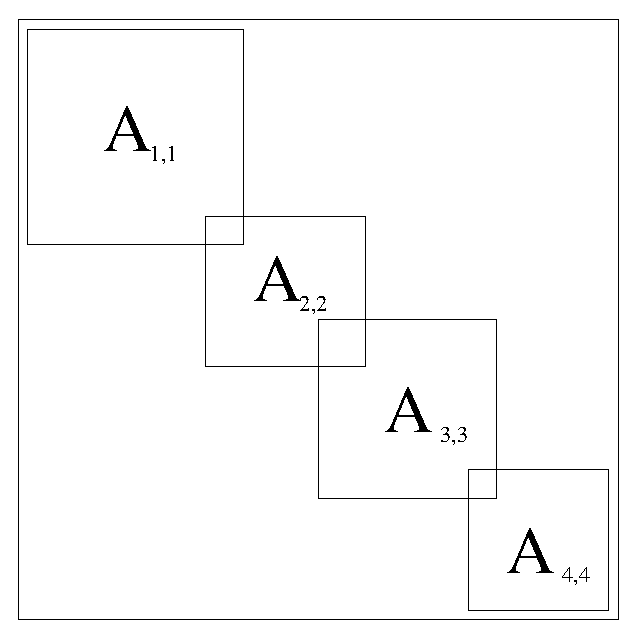
\includegraphics[width=6cm]{bj.eps}
\end{center}
\caption{The block Jacobi matrix with overlapping blocks.}
\label{fig:bj}
\end{figure}

The (damped) block Gauss-Seidel algorithm easily derives from
(\ref{eq:gen_b_jacobi}), by immediately updating the solution vector to
compute the residual. The algorithm is as follows:
\begin{eqnarray}
&& \mbox{On each processor, for each block $i$, Do} \\
&& \label{eq:gen_b_gs}
x^{(k)} = x^{(k-1)} + \omega V_i^T A_{i,i}^{-1} V_i(b - A x^{(k)}).
\end{eqnarray}

%-----------------------------------------------------------------------------
\subsection{Incomplete Factorization Preconditioners}
\label{sec:ilu}
%-----------------------------------------------------------------------------

A broad class of effective preconditioners is based on incomplete
factorization of the linear system matrix.  Such preconditioners are often
referred to as incomplete lower/upper (ILU) preconditioners.  
ILU preconditioning techniques lie between direct and
iterative methods and provide a balance between reliability and
numerical efficiency.  ILU preconditioners are constructed in the factored form
$P=\tilde{L} \tilde{U}$, with $\tilde{L}$ and $\tilde{U}$ being lower
and upper triangular matrices. Solving with $P$ involves two triangular
solutions.

ILU preconditioners are based on the observation
that, although most matrices $A$ admit an LU factorization $A=LU$, where $L$ is
(unit) lower triangular and $U$ is upper triangular, the factors $L$ and $U$ often
contain too many nonzero terms, making the cost of factorization too expensive in
time or memory use, or both.  One type of ILU preconditioner is ILU(0), which 
is defined as proceeding through the standard LU decomposition computations, but keeping 
only those terms in $\tilde{L}$ that correspond to nonzero terms in the lower
triangle of $A$ and similarly keeping only those terms in $\tilde{U}$ that 
correspond to nonzero terms in the upper triangle of $A$.  Although effective, in
some cases the accuracy of the ILU(0) may be insufficient to yield an
adequate rate of convergence. More accurate factorizations will differ
from ILU(0) by allowing some {\em fill-in}. The resulting class of
methods is called ILU($k$), where $k$ is the level-of-fill. A
level-of-fill is attributed to each element that is processed by
Gaussian elimination, and dropping will be based on the level-of-fill.
The level-of-fill should be indicative of the size of the element: the
higher the level-of-fill, the smaller the elements.  

Other strategies consider dropping by value -- for example, dropping
entries smaller than a prescribed threshold. Alternative dropping
techniques can be based on the numerical size of the element to be
discarded. Numerical dropping strategies generally yield more accurate
factorizations with the same amount of fill-in as level-of-fill
methods. The general strategy is to compute an entire row of the
$\tilde{L}$ and $\tilde{U}$ matrices, and then keep only a certain
number of the largest
entries. In this way, the amount of fill-in is
controlled; however, the structure of the resulting matrices is
undefined. These factorizations are usually referred to as ILUT($k$).

When solving a single linear system, ILUT($k$) methods can be more effective
than ILU($k$).  However, in many situations a sequence of linear systems
must be solved where the pattern of the matrix $A$ in each system is
identical but the values of changed.  In these situations, ILU($k$) is 
typically much more effective because the pattern of ILU($k$) will also
be the same for each linear system and the overhead of computing the
pattern is amortized.

%-----------------------------------------------------------------------------
\subsection{Additive Schwarz Preconditioners}
\label{sec:additive}
%-----------------------------------------------------------------------------

\ifpack\ makes very easy to define and use domain decomposition
preconditioners of (overlapping) Schwarz type.

The basic idea of DD methods is to decompose the
computational domain $\Omega$ into $M$ smaller parts $\Omega_i$,
$i=1,\ldots,M$, called subdomains, such that $\cup_{i=1}^{M}
\overline{\Omega_i} = \overline{\Omega}$.  Next, the original problem can
be reformulated within each subdomain $\Omega_i$, of smaller size. This
family of subproblems is coupled one to another through the values of the
unknown solution at subdomain interface. This coupling is then removed at
the expense of introducing an iterative process which involves, at each
step, solutions on the $\Omega_i$ with additional interface conditions on
$\partial \Omega_i \setminus \partial \Omega$.

In overlapping Schwarz preconditioner, the computational domain is
subdivided into {\sl overlapping} subdomains, and local Dirichlet-type
problems are then solved on each subdomain.  The communication between the
solutions on the different subdomains is here guaranteed by the overlapping
region. 

The additive Schwarz preconditioner can be written as:
\begin{equation}
\label{eq:as}
P_{AS}^{-1} = \sum_{i=1}^M P_i A_i^{-1} R_i ,
\end{equation}
where $M$ is the number of subdomains (that is, the number of processors in
the computation), $R_i$ is an operator that restricts the global 
vector to the vector lying on subdomain $\Omega_i$, $P_i$ is an operator that
prolongate from subdomain $\Omega_i$ to $\Omega$, and
\begin{equation}
\label{eq:Ai}
A_i = R_i A P_i.
\end{equation}

\ifpack\ supports two major cases:
\begin{itemize}
\item Minimal-overlap (here referred to as "zero-overlap"): each subdomain
is identified by the set of local rows of the preconditioned matrix;
\item Wider overlap: each subdomain is identified by the set of local rows
of a suitable overlapping matrix.
\end{itemize}
In both cases, each processor is responsible for exactly one subdomain.

In the minimal overlap case, the $R_i$'s and $P_i$'s are not implemented, since the
required components of the residual vector are already local. Besides, matrix
(\ref{eq:Ai}) can be easily extracted from the local matrix, by dropping all
nonzeros corresponding to non-local columns with no 
communications between processors. If a wider overlap
is used, instead, each application of $R_i$ and $P_i$ may require the
importing or exporting of
off-process data, and the construction of (\ref{eq:Ai}) requires
communications.

\smallskip

Once matrices (\ref{eq:Ai}) have been formed, the user still need to define a
strategy to apply the inverse of $A_i$ in (\ref{eq:as}). At this purpose,
any \ifpack\ preconditioner can be adopted. Common choices are:
\begin{itemize}
\item To solve exactly on each subdomain with an complete LU factorization, using the \verb!Ifpack_Amesos!
preconditioner. This is shown in Section~\ref{sec:as_amesos}.
\item To solve using an incomplete LU factorization, as presented in
Section~\ref{sec:as_ilu}.
\item To furtherly decompose the local domain into smaller subdomains,
  then apply a block Jacobi or block Gauss-Seidel preconditioner. This is
  outlined in Section~\ref{sec:as_b_ov}.
\end{itemize}

\begin{remark}
Additive Schwarz preconditioners as reported in equation~(\ref{eq:as}) 
are not scalable: their convergence rate
deteriorates as the number of subdomains (that is, of the processors)
increases. Algebraic techniques
exist to add an algebraic coarse level correction to~(\ref{eq:as}) to make the
preconditioner scalable; 
see for example the documentation of the ML
package~\cite{ml-guide}.
\end{remark}

%-----------------------------------------------------------------------------
\section{General Description of \ifpack\ Preconditioners}
\label{sec:prec}
%-----------------------------------------------------------------------------

All \ifpack\ preconditioners described in this document
are reported in Table~\ref{tab:all_prec}. They are all derived from the 
\verb!Ifpack_Preconditioner!
class.

%\begin{figure}
%\begin{center}
%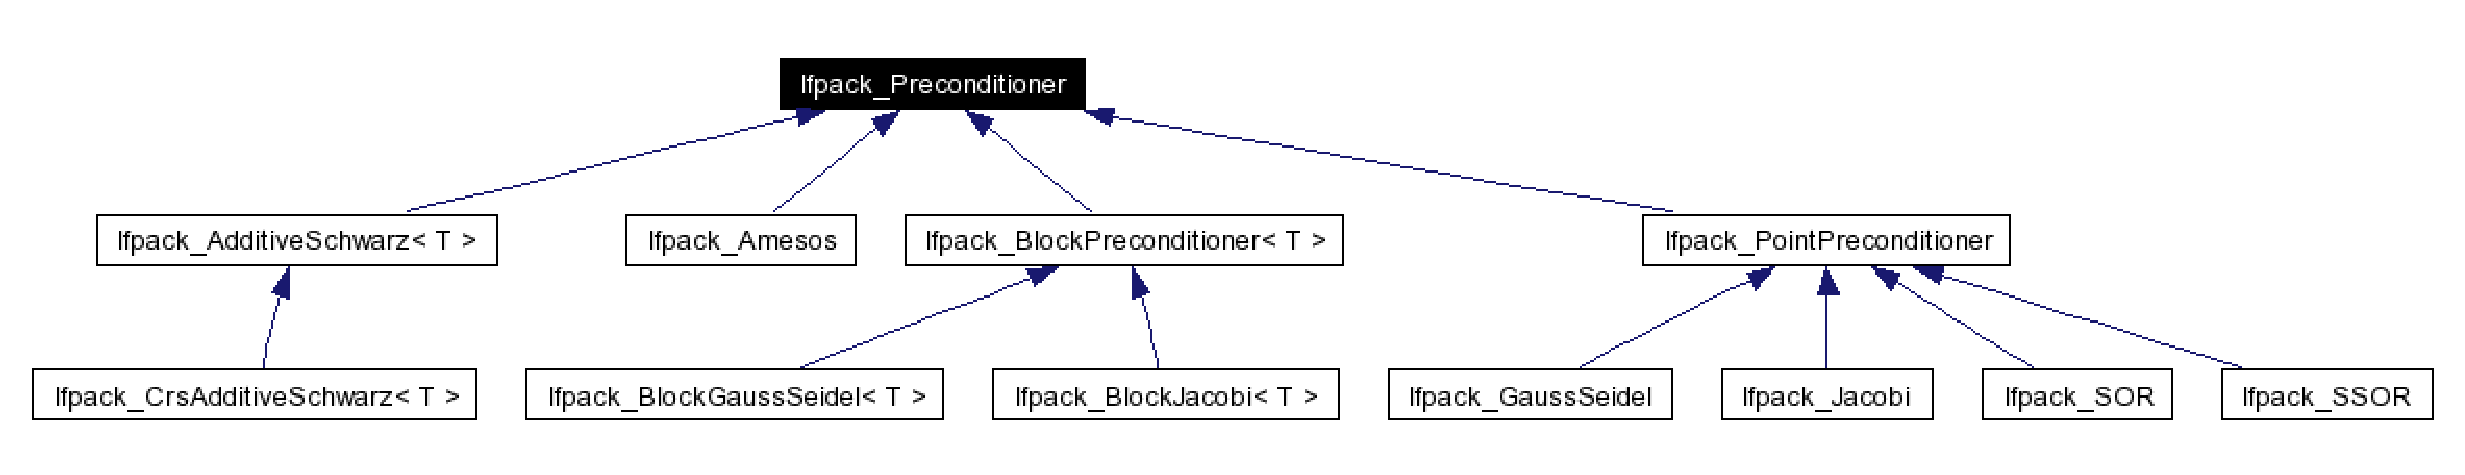
\includegraphics[width=15cm]{Ifpack_Preconditioner.eps}
%\caption{FIXME: UML diagram of  several \ifpack\ preconditioners.}
%\label{fig:if_prec}
%\end{center}
%\end{figure}

\begin{sidewaystable}
\begin{center}
\begin{tabular}{|p{6cm} | c |p{12cm} |}
\hline
Class name & Overlap & Description \\
\hline
\hline
\verb!Ifpack_PointRelaxation!   & 0 & Point (damped) relaxation
preconditioners (Jacobi, Gauss-Seidel, symmetric Gauss-Seidel). Users
can specify the number of Jacobi steps (sweeps), and the damping factor. See
Section~\ref{sec:jacobi} \\
\hline
\verb!Ifpack_BlockRelaxation! & 0 & Block relaxation
preconditioner (Jacobi, Gauss-Seidel, symmetric Gauss-Seidel). Users can store the diagonal blocks as dense or sparse. In the
latter case, any \ifpack\ preconditioner can be used to apply the inverse of
the diagonal block. See Section~\ref{sec:block}. \\
\hline
\verb!Ifpack_AdditiveSchwarz! & user & Generic additive Schwarz
preconditioner. Allows for generic additive Schwarz preconditioners, with
minimal or wider overlap. In the latter case, the user must provide
the overlapping matrix. Any \ifpack\ preconditioner can be used to
solve the local problems. See Section~\ref{sec:additive}. \\
\hline
\verb!Ifpack_IC! & 0 & Incomplete Cholesky factorization, with dropping based
on the level-of-fill of the graph. \\
\hline
\verb!Ifpack_ICT! & 0 & Incomplete Cholesky factorization, with dropping based
on threshold.\\
\hline
\verb!Ifpack_ILU! & 0 & Incomplete LU factorization, with dropping based
on the level-of-fill of the graph. \\
\hline
\verb!Ifpack_ILUT! & 0 & Incomplete LU factorization, with dropping based
on threshold. \\
\hline
\hline
\end{tabular}
\caption{Description of all the \ifpack\ preconditioners reported in this
  document. In the Table, `Overlap' indicates the overlap (with 0 being the
  minimal overlap case, `any' means that the code can construct the
  overlapping matrix for any given positive value).}
\label{tab:all_prec}
\end{center}
\end{sidewaystable}

\verb!Ifpack_Preconditioner! is a pure virtual class, derived from
\verb!Epetra_Operator!, that standarizes the construction and usage of \ifpack\
preconditioners. In fact, all \ifpack\ preconditioners are supposed to behave
as follows:
\begin{enumerate}
\item The object is constructed, passing as only input argument the
pointer of the matrix to be preconditioned, say {\tt A}. {\tt A} has already
been {\tt FillComplete()}'d\footnote{It is supposed that the {\tt OperatorDomainMap()}, {\tt the OperatorRangeMap()}
and
the {\tt RowMatrixRowMap()} of the matrix all coincide, and that each row is ass
igned
to exactly one process..}.
%
\item All the parameters, stored in a \teuchos\ parameters list, are
set using method \verb!SetParameters()!. If \verb!SetParameters()! is not
called, default values will be used.
%
\item The preconditioner is initialized by calling method \verb!Initialize()!.
In this phase, all operations that do not require the matrix values of {\tt A}
are performed (that is, only the structure of {\tt A} is used).
%
\item The preconditioner is constructed by calling method \verb!Compute()!.
In this phase, all the operations that require the matrix values of {\tt A}
are performed
\footnote{For example, in a time dependent setting, if the structure of {\tt
  A} does not change from a given time step to the next but its values do,
  the user can call {\tt Initialize()} only once before the first time step,
  then {\tt Compute()} at each time step. Also calls {\tt Initialize()} if
  not already done by the user.}
%
\item Method \verb!ApplyInverse()! applies the preconditioner. Any class that
uses \verb!ApplyInverse()! to apply the preconditioner can take advantage of
an \verb!Ifpack_Preconditioner! derived object\footnote{For example, {\tt
  AztecOO} objects can use {\tt Ifpack\_Preconditioner} objects as
    preconditioners. Note that {\tt Compute()} must be successfully called before using
    \verb!ApplyInverse()!.}

\item Method \verb!IsInitialized()! returns {\tt true} is the preconditioner has
been successfully initialized, {\tt false} otherwise.
%
\item Method \verb!IsComputed()! returns {\tt true} is the preconditioner has
been successfully computed, {\tt false} otherwise.
%
\item Method \verb!Condest()! returns an estimation of the condition
number of the preconditioned system.
The condition of a matrix $B$, called $cond_p(B)$, is defined as
$cond_p(B) = \|B\|_p\|B^{-1}\|_p$ in some appropriate norm $p$. 
$cond_p(B)$
gives some indication of how many accurate floating point
digits can be expected from operations involving the matrix and its
inverse.  A condition number approaching the accuracy of a given
floating point number system, about 15 decimal digits in IEEE double
precision, means that any results involving $B$ or $B^{-1}$ may be
meaningless.

The $\infty$-norm of a vector $y$ is defined as the maximum of the
absolute values of the vector entries, and the $\infty$-norm of a
matrix C is defined as
$\|C\|_\infty = \max_{\|y\|_\infty = 1} \|Cy\|_\infty$.
A crude lower bound for the $cond_\infty(C)$ is
$\|C^{-1}e\|_\infty$ where $e = (1, 1, \ldots, 1)^T$.  It is a
lower bound because $cond_\infty(C) = \|C\|_\infty\|C^{-1}\|_\infty
\ge \|C^{-1}\|_\infty \ge |C^{-1}e\|_\infty$. 

More accurate (and expensive) computations for the condition number can be
obtained by calling {\tt Condest(Ifpack\_CG)} or {\tt
  Condest(Ifpack\_GMRES)}\footnote{We note that using CG or GMRES to compute
and estimated condition number is an expensive operations, and should not
be used unless the accurate value of the condition number is required.}.
%
\item Methods \verb!NumInitialize()!, \verb!NumCompute()! and
\verb!NumApplyInverse()! return the number of calls to each phase.
%
\item Methods \verb!InitializeTime()!, \verb!ComputeTime()! and
\verb!ApplyInverseTime()! return the number of CPU-time spent in each phase.
%
\item Methods \verb!InitializeFlops()!, \verb!ComputeFlops()! and
\verb!ApplyInverseFlops()! return the number floating point operations (FLOPS)
  occurred in each phase.
\end{enumerate}


\begin{remark}
Some \ifpack\ preconditioners may require to copy the input \verb!List! object
given in input to \\ \verb!SetParameters()!. In any case, the
user-provided list can go out of scope before \verb!Compute()! is called.
Note that changes to user-provided list after the call to
\verb!SetParameters()! will not affect the preconditioner,
  unless \verb!SetParameters()!  is re-called.
\end{remark}

\begin{remark}
Each \verb!Ipfack_Preconditioner! object overloads the \verb!<<! operator.
Basic information about a given preconditioner can be obtained by simply
using an instruction of the type: \verb!cout << Prec!.
\end{remark}

%-----------------------------------------------------------------------------
\section{The Factory Class}
\label{sec:factory}
%-----------------------------------------------------------------------------

The easiest way to use \ifpack\ is through its factory class. Let us consider
the following fragment of code:
\begin{verbatim}
#include "Ifpack.h"
...
Epetra_RowMatrix* A; // A is already FillComplete()'d
...
Ifpack Factory;
Ifpack_Preconditioner* Prec;
string PrecType = "ILU";
int OverlapLevel = 0;
// create the preconditioner using Create()
Prec = Factory.Create(PrecType, A, OverlapLevel);
assert (Prec != 0);

// specify parameters for ILU
Teuchos::ParameterList List;
List.set("fact: level-of-fill", 5);

Prec->SetParameters();
Prec->Initialize();
Prec->Compute();
...
// Let Problem be an Epetra_LinearProblem
AztecOO Solver(Problem);
Problem.SetPrec(Prec);
// now we can solve with AztecOO
\end{verbatim}

The list of options for {\tt PrecType} is reported in
Table~\ref{tab:factory}. Note that only one word in the above fragment of code
has to be changed to define, for instance, the Gauss-Seidel preconditioner.

\begin{table}
\begin{center}
\begin{tabular}{|p{5cm} | |p{10cm} |}
\hline
{\tt PrecType} & Description \\
\hline
\hline
\tt point relaxation & Point relaxation preconditioner, like Jacobi, Gauss-Seidel,
  and symmetric Gauss-Seidel.\\
\hline
\tt block relaxation & Block relaxation preconditioner, like Jacobi, Gauss-Seidel,
  and symmetric Gauss-Seidel. LAPACK is used to apply the inverse of each
  diagonal block. \\
\hline
\tt block relaxation (Amesos) & Block relaxation preconditioner, like Jacobi, Gauss-Seidel,
  and symmetric Gauss-Seidel. Amesos is used to apply the inverse of each
  block. Requires \ifpack\ support for \amesos. \\
\hline
\tt IC & Incomplete Cholesky factorization on each subdomain. \\
\hline
\tt ICT & Incomplete Cholesky factorization with threshold on each subdomain. \\
\hline
\tt ILU & Incomplete LU factorization on each subdomain. \\
\hline
\tt ILUT & Incomplete LU with threshold on each subdomain. \\
\hline
\tt Amesos & Complete LU factorization on each subdomain. Requires \ifpack\
  support for \amesos. \\
\hline
\end{tabular}
\end{center}
\caption{List preconditioners supported by the Factory class.}
\label{tab:factory}
\end{table}

%-----------------------------------------------------------------------------
\section{Examples of Usage}
\label{sec:usage}
%-----------------------------------------------------------------------------

This section contains several examples of usage of \ifpack\ preconditioners. A
detailed list of \ifpack\ parameters is reported in
section~\ref{sec:parameters}.

%-----------------------------------------------------------------------------
\subsection{Point Preconditioners}
\label{sec:point_ex}
%-----------------------------------------------------------------------------

An example of usage of point relaxation preconditioners (in this case, Gauss-Seidel) is as
follows:
\begin{verbatim}
#include "Teuchos_ParameterList.hpp"
#include "Ifpack_PointRelaxation.h"
\end{verbatim}
Let \verb!A! be a pointer to an \verb!Epetra_RowMatrix! derived object,
  and let \verb!Problem! be a pointer to an \verb!Epetra_LinearProblem!.
We suppose that \verb!A! and 
\verb!Problem! are properly set, and
method \verb~FillComplete()~ has been called. At this point, we can create the
preconditioner as
\begin{verbatim}
Teuchos::ParameterList List;
List.set("relaxation: type", "Gauss-Seidel");

Ifpack_PointRelaxation Prec(A);

IFPACK_CHK_ERR(Prec.SetParameters(List));
IFPACK_CHK_ERR(Prec.Initialize());
IFPACK_CHK_ERR(Prec.Compute());
\end{verbatim}
Now, we can set the IFPACK preconditioner for AztecOO:
\begin{verbatim}
AztecOO AztecOOProblem(Problem);
AztecOOProblem.SetPrecOperator(Prec);
\end{verbatim}
as call \verb!AztecOO.Iterate()! as required.

Macro \verb!IFPACK_CHK_ERR()! can be used to check return values. If the
return value if different from 0, the macro prints out a warning message on
\verb!cerr!, and returns.

%-----------------------------------------------------------------------------
\subsection{Block Preconditioners}
\label{sec:block_ex}
%-----------------------------------------------------------------------------

From the point of view of the implementation block preconditioner
are sensibly more complex than their point counterpart:
\begin{enumerate}
\item A strategy to define the blocks has to be chosen (for instance, 
a linear partitioner, or a graph decomposition algortithm);
\item block Jacobi and block Gauss-Seidel algorithms require the application
of the inverse of each diagonal block $A_{i,i}$. Blocks of small dimension
should be stored as dense matrices, while larger blocks require sparse
storage. In this latter case, to apply the inverse of the block can be
reformulated as applying a preconditioner for matrix
$A_{i,i}$.
The code must allow for different choices of block preconditioners.
\end{enumerate}

\smallskip

Let us start with the definition of the blocks. 
\ifpack\ provides the following options:
\begin{itemize}
\item a linear partitioning, using class \verb!Ifpack_LinearPartitioner!;
\item a simple greedy algorithm, using class \verb!Ipfack_GreedyPartitioner!;
\item an interface to METIS, using class \verb!Ifpack_METISPartitioner!.
\end{itemize}
It is important to note that all blocks are {\sl local} -- that is, 
  all partitioner schemes will {\sl always} decompose the local graph 
  only\footnote{If used in conjuction with class {\tt Ifpack\_AdditiveSchwarz},
    blocks can span more than one processor.}.

All \ifpack\ partitioners are derived from the pure virtual class
\verb!Ifpack_Partitioner!, and all require in the constructor phase
an \verb!Ifpack_Graph! object. \verb!Ifpack_Graph!'s can be easily
created (as light-weigth) conversions from \verb!Epetra_RowMatrix!'s
and \verb!Epetra_CrsGraph!'s, as follows At this point, we can create the
preconditioner as
\begin{verbatim}
#include "Ifpack_Graph.h"
#include "Ifpack_Graph_Epetra_CrsGraph.h"
#include "Ifpack_Graph_Epetra_RowMatrix.h"

// use either CsrA or RowA, depending on your application
Epetra_CrsMatrix* CrsA;
Epetra_RowMatrix* RowA;

Ifpack_Graph CrsGraph* CrsGraph =
  new Ifpack_Graph_CrsGraph(&(CrsA->Graph()));

Ifpack_Graph RowGrap* RowGraph  =
  new Ifpack_Graph_RowMatrix(RowA);
\end{verbatim}
Note that the \verb!Partitioner! object will decompose the graph (either
\verb!CrsGraph! or \verb!RowGraph!) into
non-overlapping sets (that is, each graph vertex is assigned to exactly one
set).

The following fragment of code shows how to use a greedy partitioner to define
4 local blocks for a given \verb!Ifpack_Graph!.

\begin{verbatim}
#include "Ifpack_Graph.h"
#include "Ifpack_GreedyPartitioner.h"
#include "Ifpack_BlockRelaxation.h"
#include "Teuchos_ParameterList.hpp"
...

Ifpack_Graph* Graph;   
// Graph is created here

Teuchos::ParameterList List;
List.set("partitioner: local parts", 4);
Ifpack_Partitioner* Partitioner = new Ifpack_GreedyPartitioner(Graph);

// set the parameters (in this case the # of blocks only)
Partitioner->SetParameters(List);

// compute the partition
Partitioner->Compute();
\end{verbatim}

Once an \verb!Ifpack_Partitioner! is created, we are ready to
compute the block preconditioner. This requires the extraction of
all the diagonal bocks of equation (\ref{eq:D}). In \ifpack, the
user can choose to store the $A_{i,i}$ as dense matrices, or a sparse
matrices. In the former case, the inverse of each block is applied using
LAPACK\footnote{LAPACK is used to factorize the matrix, then each application
  of $A_{i,i}^{-1}$ results in a dense linear system solution.}. In the
  latter, the user can specify any valid \verb!Ifpack_Preconditioner!.

As an example, we now create a block Jacobi preconditioner for 
a given \verb!Epetra_RowMatrix!, say \verb!A!,
with damping parameter of 0.67, and 2 sweeps. Each diagonal block is stored as a dense
matrix.

\begin{verbatim}
#include "Ifpack_BlockRelaxation.h"
#include "Ifpack_DenseContainer.h"
...

Ifpack_Partitioner* Partitioner;
// Partitioner is created here

Ifpack_Preconditioner* Prec =
  new Ifpack_BlockRelaxation<Ifpack_DenseContainer>(A);

Teuchos::ParameterList List;
List.set("relaxation: sweeps", 2);
List.set("relaxation: damping parameter", 0.67);
Prec->SetParameters(List);
Prec->Compute();
\end{verbatim}
The previous example makes use of a dense containers to store
the diagonal blocks.
In \ifpack, a {\sl container} is an object that contains all the necessary
data to solve the linear system with any given $A_{i,i}$. 
\verb!Ifpack_DenseContainer! stores each $A_{i,i}$ as
\verb!Epetra_SerialDenseMatrix!. Alternatively, one can use 
\verb!Ipfack_SparseContainer! to store each block as an
\verb!Epetra_CrsMatrix!. Sparse containers are templated with an
\verb!Ifpack_Preconditioner!, so that the user can specify which \ifpack\
  preconditioner has to be used to apply the inverse of each sparse block.

The following fragment of code illustrates how to use the direct factorization
of Amesos (through class \verb!Ifpack_Amesos!\footnote{This requires \ifpack\
	   to be configured with option {\tt --enable-amesos}.}) with sparse containers. The preconditioner will be a block Gauss-Seidel one.

\begin{verbatim}
#include "Ifpack_BlockRelaxation.h"
#include "Ifpack_SparseContainer.h"
#include "Ifpack_Amesos.h"
...

Ifpack_Partitioner* Partitioner;
// Partitioner is created here

Ifpack_Preconditioner* Prec =
  new Ifpack_BlockRelaxation<Ifpack_SparseContainer<Ifpack_Amesos> >(A);

Teuchos::ParameterList List;
List.set("relaxation: sweeps", 2);
List.set("amesos: solver type", "Amesos_Klu");
Prec->SetParameters(List);
Prec->Initialize();
Prec->Compute();
\end{verbatim}

Option \verb!amesos: solver type! specifies the \amesos\ solver that
has to be adopted. If the selected solver is not available, then
\verb!Ifpack_Amesos! will create an \verb!Amesos_Klu! solver\footnote{KLU is
  compiled by default with \amesos. Please consult the \amesos\ documentation
    for more details.}.
As {\sl any} \ifpack\ preconditioner can be used, one can also adopt, for
instance, a point Gauss-Seidel algorithm in each block:
\begin{verbatim}
Ifpack_Preconditioner* Prec =
  new Ifpack_BlockRelaxation<Ifpack_SparseContainer<Ifpack_GaussSeidel> >(A);
\end{verbatim}

A call to \verb!SetParameters(List)! will set the parameters for the block
preconditioner.

%-----------------------------------------------------------------------------
\subsection{Additive Schwarz with Exact Local Solves}
\label{sec:as_amesos}
%-----------------------------------------------------------------------------

The following fragment of code shows the use of additive preconditioners. The
local subproblems with matrix $A_i$ are solved using a (complete) LU
factorization through \amesos.
\begin{verbatim}
#include "Ifpack_AdditiveSchwarz.h"
#include "Ifpack_Amesos.h"

Epetra_RowMatrix* A;
// Here the elements of A are filled, and FillComplete() is called.

int OverlapLevel = 0;
Ifpack_Preconditioner* Prec = 
  new Ifpack_AdditiveSchwarz<Ifpack_Amesos>(A, OverlapLevel);

Teuchos::ParameterList List;
IFPACK_CHK_ERR(Prec->SetParameters(List));
IFPACK_CHK_ERR(Prec->Initialize());
IFPACK_CHK_ERR(Prec->Compute());
\end{verbatim}

\begin{remark}
Complete factorizations can be expensive to compute, especially for problems
arising from discretizations on 3D grids. The user should consider complete
factorizations if the local problems are small, or when other, cheaper
preconditioners fail.
\end{remark}

%-----------------------------------------------------------------------------
\subsection{Additive Schwarz with ILU}
\label{sec:as_ilu}
%-----------------------------------------------------------------------------

The following fragment of code shows the use of additive preconditioners. The
local subproblems with matrix $A_i$ are solved using an incomplete
factorization.
\begin{verbatim}
#include "Ifpack_AdditiveSchwarz.h"
#include "Ifpack_ILU.h"

Epetra_RowMatrix* A;
// Here the elements of A are filled, and FillComplete() is called.

int OverlapLevel = 0;
Ifpack_Preconditioner* Prec = 
  new Ifpack_AdditiveSchwarz<Ifpack_ILU>(A, OverlapLevel);

Teuchos::ParameterList List;
List.set("fact: level of fill", 2);
IFPACK_CHK_ERR(Prec->SetParameters(List));
IFPACK_CHK_ERR(Prec->Initialize());
IFPACK_CHK_ERR(Prec->Compute());
\end{verbatim}

The difficulty with this type of preconditioner is that it tends to become
less robust and require more iterations as the number of processors used
increases.  This effect can be offset to some extent by allowing {\em
overlap}.  Overlap refers to having processors redundantly own certain rows
of the matrix for the ILU factorization.  Level-1 overlap is defined so
that a processor will include rows that are part of its original set.  In
addition, if row $i$ is part of its original set and row $i$ of $A$ has a
nonzero entry in column $j$, then row $j$ will also be included in the
factorization on that processor.  Other levels of overlap are computed
recursively.  IFPACK supports an arbitrary level of overlap.  However,
level-1 is often most effective.  Seldom more than 3 levels are needed. 

\smallskip

The user can access the factorization of the local matrix produced by
templating \verb!Ifpack_AdditiveSchwarz! with classes \verb!Ifpack_IC!,
  \verb!Ifpack_ICT!, \verb!Ifpack_ILU! and \verb!Ifpack_ILUT! in the following
  way:
\begin{verbatim}
Ifpack_Preconditioner* Prec = 
  new Ifpack_AdditiveSchwarz<Ifpack_ILU>(A, OverlapLevel);

Ifpack_ILU* Inverse = Prec->Inverse();
\end{verbatim}
Then, the total number of nonzeros in the L and U factors can be queried as
follows:
\begin{verbatim}
int NumGlobalNonzerosLU = Inverse->NumGlobalNonzeros();
\end{verbatim}
The L and U factors are stored as \verb!Epetra_CrsMatrix!'s, whose pointers
can be obtained as follows\footnote{For classes {\tt Ifpack\_IC} and {\tt
  Ifpack\_ICT} the user shall use method {\tt H()}.}:
\begin{verbatim}
const Epetra_CrsMatrix& L = Inverse->L();
const Epetra_CrsMatrix& U = Inverse->U();
\end{verbatim}

%-----------------------------------------------------------------------------
\subsection{Additive Schwarz with Local Block Preconditioners}
\label{sec:as_b_ov}
%-----------------------------------------------------------------------------

Another possible technique to apply the inverse of $A_i$ in (\ref{eq:as})
is to adopt a block preconditioner, like block Jacobi 
or block Gauss-Seidel (see
Section~\ref{sec:block}). This requires a
bit more work, as we have to specify the partitioner, and the container. Let
us start with dense containers.

The required include files are:
\begin{verbatim}
#include "Ifpack_AdditiveSchwarz.h"
#include "Ifpack_BlockPreconditioner.h"
#include "Ifpack_Graph_Epetra_RowMatrix.h"
#include "Ifpack_DenseContainer.h"
\end{verbatim}

Let \verb!A! be an \verb!Epetra_RowMatrix!. We suppose that
\verb!FillComplete()! has been called. 

As always, we create a parameters list, that will be used
for all \ifpack\ objects:
\begin{verbatim}
Teuchos::ParameterList List;
\end{verbatim}
At this point we can create the block Jacobi preconditioner as follows:
\begin{verbatim}
Ifpack_Preconditioner* Prec = 
  new Ifpack_AdditiveSchwarz<
    Ifpack_BlockPreconditioner<Ifpack_DenseContainer> >(A);

Prec->SetParameters(List);
Prec->Initialize();
Prec->Compute();
\end{verbatim}
As we have used {\tt Ifpack\_DenseContainer}, blocks are stored are dense
matrices, and LAPACK is used to apply the inverse of each block. This can be a
limiting factor for large blocks. In this latter case, it is preferable to
store the blocks are sparse matrices, and use a sparse solver to apply their
inverse. This can be done by resorting to {\tt Ifpack\_SparseContainer}. 
Sparse containers can be used with minor modifications. The only difference is
that we also have to specify how to apply the inverse of each block, for
instance using the exact factorizations of \amesos:
\begin{verbatim}
Ifpack_Preconditioner* Prec = 
  new Ifpack_AdditiveSchwarz<Ifpack_BlockPreconditioner
    <Ifpack_SparseContainer<Ifpack_Amesos> > >(A);
\end{verbatim}

Should the user want to use a block Gauss-Seidel preconditioner (where each
block is defined by partitioning the local graph of the overlapping matrix),
he/she could proceed as follows:
\begin{verbatim}
Teuchos::ParameterList List;
List.set("relaxation: damping factor", .67);
List.set("relaxation: sweeps",5);
List.set("partitioner: local parts", 4);
List.set("partitioner: overlap", OverlapLevel);

Epetra_RowMatrix* A; // A is FillComplete()'d.

Ifpack_Preconditioner* Prec =
  new Ifpack_AdditiveSchwarz<Ifpack_BlockPreconditioner
      <Ifpack_SparseContainer<Ifpack_Amesos> > >(A,OverlapLevel);

IFPACK_CHK_ERR(Prec->SetParameters(List));
IFPACK_CHK_ERR(Prec->Compute());
\end{verbatim}

%-----------------------------------------------------------------------------
\section{Parameters for \ifpack\ preconditioners}
\label{sec:parameters}
%-----------------------------------------------------------------------------

The parameters that affect the \ifpack\ preconditioners are reported
below. It is important to note that parameters for all \ifpack\
preconditioners must be spelled as indicated:
misspelled parameters will be ignored, parameters are case sensitive, and words
  are separated by one space only.

\smallskip

For more details about the \teuchos\ parameters list we refer to the
\teuchos\ documentation.  Table~\ref{tab:teuchos} briefly reports the most
important methods of this class.
\ifpack\ requires just a very basic usage of the parameters list.
Input parameters are set via method \verb!set(Name,Value)!, where
\verb!Name! is a string containing the parameter name, and \verb!Value! is the
specified parameter value, whose type can be any C++ object or pointer. 

\begin{table}[htbp]
  \centering
  \begin{tabular}{| p{4cm} | p{10cm} |}
    \hline
    \verb!set(Name,Value)! & Add entry \verb!Name! with value and type
    specified by \verb!Value!. Any C++ type (like int, double, a
    pointer, etc.) is valid. \\
    \verb!get(Name,DefValue)! & Get value (whose type is automatically
    specified by \verb!DefValue!). If not present, return
    \verb!DefValue!. \\
    \verb!subList(Name)! & Get a reference to sublist \verb!List!. If not
    present, create the sublist. \\
    \hline
  \end{tabular}
  \caption{Some methods of Teuchos::ParameterList class.}
  \label{tab:teuchos}
\end{table}

\smallskip

\choicebox{\tt relaxation: type}{[{\tt string}] Relaxation scheme. Valid
  choices are: {\tt Jacobi}, {\tt Gauss-Seidel}, {\tt symmmetric
    Gauss-Seidel}. Default: {\tt Jacobi}.}

\choicebox{\tt relaxation: sweeps}{[{\tt int}] Number of sweeps of
  the point relaxation preconditioner. Default: {\tt 1}.}

\choicebox{\tt relaxation: damping factor}{[{\tt double}] This is the value for $\omega$ 
  in formulae (\ref{eq:jacobi}), (\ref{eq:gs}), (\ref{eq:sor}) and
    (\ref{eq:ssor}). Default: {\tt 1.0}.}
				 
\choicebox{\tt relaxation: min diagonal value}{[{\tt double}] Replace diagonal
  values whose absolute value is less than the specified value by this value
    (for point relaxation methods only). Default: {\tt 1e-9}.}

\choicebox{\tt relaxation: zero starting solution}{[{\tt bool}] 
  If {\tt true}, the input values in the preconditioned vector will be used as
    starting solution (for relaxation methods only).  Default: {\tt true}.}

\choicebox{\tt partitioner: type}{[{\tt string}] Defines how to build the
  local blocks (for block relaxation methods). Valid choices are:
  {\tt linear} (use a simple linear decomposition), {\tt greedy} 
  (use a greedy algorithm to partition the local graph), 
  or {\tt metis} (call METIS on the local graph). Default: {\tt linear}.}

\choicebox{\tt partitioner: local parts}{[{\tt int}] Number of (local)
  subgraphs (for block relaxation methods only). Default: 4.}

\choicebox{\tt partitioner: overlap}{[{\tt int}] Overlap among blocks. Only
  for block Jacobi methods. Default: 0.}

\choicebox{\tt partitioner: root node}{[{\tt int}] Root node, for greedy
  algorithm only. Default: 0}

\choicebox{\tt schwarz: combine mode}{[{\tt Epetra\_CombineMode}].
Default: {\tt Zero}.
It can assume one of the following values:
{\tt Add}: Components on the receiving processor will be added together;
{\tt Zero}: Off-processor components will be ignored;
{\tt Insert}: Off-processor components will be inserted into locations on
receiving processor replacing existing values.
{\tt Average}: Off-processor components will be averaged with existing;
{\tt AbsMax}: Magnitudes of Off-processor components will be
maxed with magnitudes of existing components on the receiving
processor. Note that, for non-zero overlap values, the preconditioner is in general
  non-symmetric, due to the handling of the overlapping region. Set this parameter to {\tt Insert} if a
    symmetric preconditioner is required.}

\choicebox{\tt amesos: solver type}{[{\tt string}]. Defines the Amesos solver to be
  used by class Ifpack\_Amesos. Valid values are:
{\tt Amesos\_Lapack},
{\tt Amesos\_Klu},
{\tt Amesos\_Umfpack},
{\tt Amesos\_Superlu},
{\tt Amesos\_Mumps},
{\tt Amesos\_Dscpack}. Default: {\tt Amesos\_Klu} Default: {\tt Amesos\_Klu}.}

\choicebox{\tt fact: level-of-fill}{[{\tt int}] Level-of-fill for IC and ILU.}

\choicebox{\tt fact: ict level-of-fill}{[{\tt double}] Level-of-fill for ICT.}

\choicebox{\tt fact: ilut level-of-fill}{[{\tt double}] Level-of-fill for
  ILUT.}

\choicebox{\tt fact: relax value}{[{\tt double}] Relaxation value.}

\smallskip

It is often convenient to compute the incomplete factorization of a given
matrix, say $A$, by ``filtering'' this matrix, so that it behaves ``well''
during the factorization process. The idea to filter the matrix is very
simple: instead of using matrix $A$, we perform the factorization  on 
a modified matrix $B$\footnote{This matrix is never built. The code modifies
  the {\tt ExtractMyRowCopy()} method, and updated the diagonal value.}, whose elements are defined as
\begin{equation}
\label{eq:B}
\begin{array}{lcr}
B_{i,j} = A_{i,j} \quad \quad i \neq j \\
B_{i,i} = \alpha \; \; sgn(A_{i,i}) + \rho A_{i,i},
  \end{array}
\end{equation}
where $\alpha$ and $\rho$ are two real parameters, to be determined by the
user. $\alpha$ represents and absolute threshold added to the matrix, while
$\rho$ is a relative threshold (that is, the actual diagonal value of the matrix to
be factored is $\rho$ times the original value). 

\smallskip

\choicebox{\tt fact: absolute threshold}{[{\tt double}] Value $\alpha$ in equation (\ref{eq:B}). }

\choicebox{\tt fact: relative threshold}{[{\tt double}] Value $\rho$ in
  equation (\ref{eq:B}). }


%-----------------------------------------------------------------------------
\section{Analysis Tools}
\label{sec:analysis}
%-----------------------------------------------------------------------------

\ifpack\ contains the following tools to analyze a linear system matrix:
\begin{itemize}
\item Function {\tt Ifpack\_Analyze()} reports some information about the
structure of the matrix, its diagonal elements, and others.
\item Function {\tt Ifpack\_PrintSparsity()} prints on a PostScript file the
sparsity pattern of a given {\tt Epetra\_RowMatrix}.
\item Function {\tt Ifpack\_PrintSparsitySimple()}, to be used only with small
matrices, prints on a screen the
sparsity pattern of a given {\tt Epetra\_RowMatrix}.
\end{itemize}

%-----------------------------------------------------------------------------
%-----------------------------------------------------------------------------
\section{Configuring and Building \ifpack}
\label{sec:config}
%-----------------------------------------------------------------------------

We recommend to configure and build \ifpack\ as part of the standard 
\trilinos~build and configure process.  In fact,
\ifpack\ is built by default if you follow the standard \trilinos~configure
and build directions. Please refer to the \trilinos~documentation 
for information about the configuration and building of
other \trilinos~packages.

\smallskip

To configure and build \ifpack\ through \trilinos, you may need do the
following (actual configuration options may vary depending on the
specific architecture, installation, and user's need).  It's assumed
that shell variable \verb!$TRILINOS_HOME!  identifies the
\trilinos~directory, and, for example, that we are compiling under LINUX
and MPI.
\begin{verbatim}
% cd $TRILINOS_HOME
% mkdir LINUX_MPI
% cd LINUX_MPI
% $TRILINOS_HOME/configure  --with-mpi-compilers \
    --prefix=$TRILINOS_HOME/LINUX_MPI
% make
% make install
\end{verbatim}

\ifpack\ is configured and built using the GNU autoconf~\cite{Autoconf} and
automake~\cite{Automake} tools. 
\ifpack configuration and compilation can be tuned by several flags.
The user may type 
\begin{verbatim}
% configure --help
\end{verbatim}
in the \ifpack\ source directory for a complete list. Here, we briefly report
the list of packages (included or not in Trilinos) that are supported 
by \ifpack:

\medskip

\choicebox{\tt --enable-amesos}
{Enables support for the \amesos~package, which can be used to solve the
  local subproblems in Schwarz-type preconditioners, or in
    block Jacobi and block Gauss-Seidel preconditioners.}

\choicebox{\tt --enable-aztecoo}
{Enable support for the \aztecoo\ package. \aztecoo~is used in several tests
  and examples.}

\choicebox{\tt --enable-teuchos}
{Enable support for the \teuchos\ package, whose parameters list is used by
  several \ifpack\ classes.}

\choicebox{\tt --enable-triutils}
{Enable support for the \triutils\ package, which is used in some examples and
  test to generate the linear system.}

\choicebox{\tt --enable-ifpack-metis}
{Enable support for the \metis\ package, version 4.0 or later. \metis\ can be
  used to create block preconditioners.}

\begin{remark}
\ifpack\ cannot be compiled without the \epetra\ library.
\end{remark}


\clearpage
\newpage
%@HEADER
% ************************************************************************
% 
%          Trilinos: An Object-Oriented Solver Framework
%              Copyright (2001) Sandia Corporation
% 
% Under terms of Contract DE-AC04-94AL85000, there is a non-exclusive
% license for use of this work by or on behalf of the U.S. Government.
% 
% This program is free software; you can redistribute it and/or modify
% it under the terms of the GNU General Public License as published by
% the Free Software Foundation; either version 2, or (at your option)
% any later version.
%   
% This program is distributed in the hope that it will be useful, but
% WITHOUT ANY WARRANTY; without even the implied warranty of
% MERCHANTABILITY or FITNESS FOR A PARTICULAR PURPOSE.  See the GNU
% General Public License for more details.
%   
% You should have received a copy of the GNU General Public License
% along with this program; if not, write to the Free Software
% Foundation, Inc., 675 Mass Ave, Cambridge, MA 02139, USA.
% 
% Questions? Contact Michael A. Heroux (maherou@sandia.gov)
% 
% ************************************************************************
%@HEADER

\section{The Teuchos Utility Classes}
\label{chap:teuchos}

Teuchos (pronounced ``te-fos'') is a collection of portable C++ tools
that facilitate the development of scientific codes.  Only a few of the many
tools in Teuchos are mentioned in this section.
For more details on all of the capabilities provided by Teuchos, please 
refer to the online documentation (\verb!http://software.sandia.gov/trilinos/packages/teuchos!).

Teuchos classes have been divided between a ``standard'' build and an
``extended'' build. The ``standard'' build contains the general purpose
templated tools like BLAS/LAPACK wrappers, parameter lists, a command-line parser,
serial dense matrices, timers, flop counters, and a reference-counted pointer class.  
These tools are built by default when Teuchos is enabled using the 
configure option \verb!--enable-teuchos!. 
The ``extended'' build contains more special purpose tools like 
XML parsing and MPI communicators, which can be included in the Teuchos
library by using the configure option \verb!--enable-teuchos-extended!.

\medskip

In this Chapter, we will present the following ``standard'' build classes:
\begin{itemize}

\item \verb!Teuchos::ScalarTraits! class (Section~\ref{sec:teuchos:ScalarTraits}):
  The ScalarTraits class provides a basic interface to scalar types (float, double, 
  complex$<$float$>$, complex$<$double$>$) that is used by the templated computational
  classes within Teuchos.  It is the mechanism by which Teuchos' capabilities 
  can be extended to support arbitrary precisions.

\item \verb!Teuchos::SerialDenseMatrix! class (Section~\ref{sec:teuchos:SDM}): 
  The SerialDenseMatrix is a templated version of the \verb!Epetra_SerialDenseMatrix! class
  that is most often used to interface with the templated BLAS/LAPACK wrappers.

\item \verb!Teuchos::BLAS! class (Section~\ref{sec:teuchos:BLAS}):
  The BLAS class provides templated wrappers
  for the native BLAS library and can be extended to support arbitrary precision
  computations.  

\item \verb!Teuchos::LAPACK! class (Section~\ref{sec:teuchos:LAPACK}):
  The LAPACK class provides templated wrappers for the native LAPACK library.

\item \verb!Teuchos::ParameterList! class (Section~\ref{sec:teuchos:ParameterList}):
  ParameterList is a container that can be used to group all the parameters required by a
  given piece of code.

\item \verb!Teuchos::RefCountPtr! class (Section~\ref{sec:teuchos:RefCountPtr}):
  RefCountPtr is a smart reference-counted pointer class, which provides a functionality
  similar to the garbage collector of Java. 

\item \verb!Teuchos::TimeMonitor! class (Section~\ref{sec:teuchos:TimeMonitor}):
  TimeMonitor is a timing class that starts a timer when it is initialized and
  stops it when the destructor is called on the class.

\item \verb!Teuchos::CommandLineProcessor! class (Section~\ref{sec:teuchos:CLP}): 
  CommandLineProcessor is a class that helps parse command line input arguments from 
  \verb!(argc,argv[])!.   
\end{itemize}

%%%
%%%
%%%

\subsection{Teuchos::ScalarTraits}
\label{sec:teuchos:ScalarTraits}

The ScalarTraits class provides a basic interface to scalar types (float, double, 
complex$<$float$>$, complex$<$double$>$) that is used by the templated 
computational classes within Teuchos.  This interface includes a definition of
the magnitude type and methods for obtaining random numbers, representations of 
zero and one, the square root, and machine-specific parameters.  
The Teuchos classes that utilize this scalar traits mechanism are 
\verb!Teuchos::SerialDenseMatrix!, \verb!Teuchos::BLAS!, and \verb!Teuchos::LAPACK!.  

ScalarTraits enables the extension of Teuchos' computational
capabilities to any scalar type that can support its basic interface.  In particular, 
this interface can be used for arbitrary precision scalar types.  An interface to the
arbitrary precision library ARPREC \cite{arprec:02} is available if Teuchos
is configured with \verb!--enable-teuchos-arprec!. Teuchos must also be configured
with the local ARPREC library paths (\verb!--with-libs!, \verb!--with-incdirs!, and 
\verb!--with-libdirs!).  To obtain more information on ARPREC or download the 
source code, see {\tt http://crd.lbl.gov/$\sim$dhbailey/mpdist/}.

\begin{remark} To enable complex arithmetic (complex$<$float$>$ or complex$<$double$>$) 
support in ScalarTraits or any dependent classes, configure Teuchos with {\tt --enable-teuchos-complex}.
\end{remark}

%%%
%%%
%%%

\subsection{Teuchos::SerialDenseMatrix}
\label{sec:teuchos:SDM}

\verb!Teuchos::SerialDenseMatrix! is a templated version of the SerialDenseMatrix class in \verb!Epetra!
(Chapter \ref{chap:epetra_mat}).  It is most useful for interfacing with the templated BLAS and 
LAPACK wrappers, which will be discussed in Sections \ref{sec:teuchos:BLAS} and \ref{sec:teuchos:LAPACK}.  
However, by enabling the simple construction and manipulation of small dense matrices, 
the SerialDenseMatrix class has also been used as an independent tool in many 
Trilinos packages.

\verb!Teuchos::SerialDenseMatrix! provides a serial interface to a small dense matrix
of templated scalar type.  This means a SerialDenseMatrix object can be created for any scalar type 
supported by Teuchos::ScalarTraits (Section \ref{sec:teuchos:ScalarTraits}).  Boundschecking
can be enabled for this class by configuring Teuchos with {\tt --enable-teuchos-abc}.
An exception will be thrown every time a matrix bound is violated by any method.  This 
incurs a lot of overhead for this class, so boundschecking is only recommended as a debugging tool.

To use the Teuchos::SerialDenseMatrix class, include the header:

{\small 
\begin{verbatim}
#include "Teuchos_SerialDenseMatrix.hpp"
\end{verbatim}}
Creating a double-precision matrix can be done in several ways:
{\small 
\begin{verbatim}
// Create an empty matrix with no dimension
Teuchos::SerialDenseMatrix<int,double> Empty_Matrix;
// Create an empty 3x4 matrix
Teuchos::SerialDenseMatrix<int,double> My_Matrix( 3, 4 );
// Basic copy of My_Matrix
Teuchos::SerialDenseMatrix<int,double> My_Copy1( My_Matrix ),
// (Deep) Copy of principle 3x3 sub-matrix of My_Matrix
                  My_Copy2( Teuchos::Copy, My_Matrix, 3, 3 ),
// (Shallow) Copy of 2x3 sub-matrix of My_Matrix
                  My_Copy3( Teuchos::View, My_Matrix, 2, 3, 1, 1 );
\end{verbatim}}
The matrix dimensions and strided storage information can be obtained:
{\small
\begin{verbatim}
int rows = My_Copy3.numRows();  // number of rows
int cols = My_Copy3.numCols();  // number of columns
int stride = My_Copy3.stride(); // storage stride
\end{verbatim}}
Matrices can change dimension:
{\small
\begin{verbatim}
Empty_Matrix.shape( 3, 3 );     // size non-dimensional matrices
My_Matrix.reshape( 3, 3 );      // resize matrices and save values
\end{verbatim}}
Filling matrices with numbers can be done in several ways:
{\small 
\begin{verbatim}
My_Matrix.random();             // random numbers
My_Copy1.putScalar( 1.0 );      // every entry is 1.0
My_Copy2(1,1) = 10.0;           // individual element access
Empty_Matrix = My_Matrix;       // copy My_Matrix to Empty_Matrix 
\end{verbatim}}
Basic matrix arithmetic can be performed:
{\small
\begin{verbatim}
Teuchos::SerialDenseMatrix<int,double> My_Prod( 3, 2 );
// Matrix multiplication ( My_Prod = 1.0*My_Matrix*My_Copy^T )
My_Prod.multiply( Teuchos::NO_TRANS, Teuchos::TRANS, 
                  1.0, My_Matrix, My_Copy3, 0.0 );
My_Copy2 += My_Matrix;         // Matrix addition
My_Copy2.scale( 0.5 );         // Matrix scaling
\end{verbatim}}
The pointer to the array of matrix values can be obtained:
{\small
\begin{verbatim}
double* My_Array = My_Matrix.values();   // pointer to matrix values
double* My_Column = My_Matrix[2];        // pointer to third column values
\end{verbatim}}
The norm of a matrix can be computed:
{\small
\begin{verbatim}
double norm_one = My_Matrix.normOne();        // one norm
double norm_inf = My_Matrix.normInf();        // infinity norm
double norm_fro = My_Matrix.normFrobenius();  // frobenius norm
\end{verbatim}}
Matrices can be compared:
{\small
\begin{verbatim}
// Check if the matrices are equal in dimension and values
if (Empty_Matrix == My_Matrix) {
  cout<< "The matrices are the same!" <<endl;
}
// Check if the matrices are different in dimension or values
if (My_Copy2 != My_Matrix) {
  cout<< "The matrices are different!" <<endl;
}
\end{verbatim}}
A matrix can be sent to the output stream:
{\small
\begin{verbatim}
cout<< My_Matrix << endl;
\end{verbatim}}
This section presents examples of all the methods in the 
{\tt Teuchos::SerialDenseMatrix} class and can be found in
\TriExe{teuchos/ex1.cpp}.  There is also a specialization of
this class for serial dense vectors that includes additional creation, accessor, 
arithmetic, and norm methods ({\tt Teuchos::SerialDenseVector}).

%%%
%%%
%%%

\subsection{Teuchos::BLAS}
\label{sec:teuchos:BLAS}

The \verb!Teuchos::BLAS! class provides templated wrappers for the native BLAS library.
This class has been written to facilitate the interface between C++ codes and BLAS,
which are written in Fortran.  Unfortunately, the interface between C++ and Fortran
function calls is not standard across all computer platforms.  The \verb!Teuchos::BLAS!
class provides C++ wrappers for BLAS kernels that are specialized during the Teuchos
configuration.  This insulates the rest of Teuchos and its users from the details of
the Fortran to C++ translation.

The \verb!Teuchos::BLAS! class provides C++ wrappers for a substantial subset of the 
BLAS kernels (Figure \ref{blas_kernels}).
The native BLAS library implementations of those kernels
will be used for the standard scalar types (float, double, complex$<$float$>$, complex$<$double$>$).  
However, \verb!Teuchos::BLAS! also has a
templated version of each of these kernels.  Paired with \verb!Teuchos::ScalarTraits! 
(Section \ref{sec:teuchos:ScalarTraits}), the \verb!Teuchos::BLAS! class can be extended 
to provide arbitrary precision computations.  
To use the \verb!Teuchos::BLAS! class, 
include the header:
{\small 
\begin{verbatim}
#include "Teuchos_BLAS.hpp"
\end{verbatim}}
Creating an instance of the BLAS class for double-precision kernels looks like:
{\small 
\begin{verbatim}
Teuchos::BLAS<int, double> blas;
\end{verbatim}}
This instance provides the access to all the BLAS kernels listed in Figure \ref{blas_kernels}:
{\small
\begin{verbatim}
const int n = 10;
double alpha = 2.0;
double x[ n ];
for ( int i=0; i<n; i++ ) { x[i] = i; }
blas.SCAL( n, alpha, x, 1 );
int max_idx = blas.IAMAX( n, x, 1 );
cout<< "The index of the maximum magnitude entry of x[] is the "
    <<  max_idx <<"-th and x[ " << max_idx-1 << " ] = "<< x[max_idx-1] 
    << endl;
\end{verbatim}}
This is a small usage example, but its purpose is to illustrate that any of the supported 
BLAS kernels is a method of the {\tt Teuchos::BLAS} class.  
This example can be found in \TriExe{teuchos/ex2.cpp}.  

\begin{figure}[hbt]\centerline{\small{
\begin{tabular}{|l||l|}\hline
\bf{BLAS Kernel} & \bf{Description} \\\hline\hline
\_ROTG & Computes a Givens plane rotation \\\hline
\_SCAL & Scale a vector by a constant \\\hline
\_COPY & Copy one vector to another \\\hline
\_AXPY & Add one scaled vector to another \\\hline
\_ASUM & Sum the absolute values of the vector entries \\\hline
\_DOT  & Compute the dot product of two vectors \\\hline
\_NRM2 & Compute the 2-norm of a vector \\\hline
\_IAMAX & Determine the index of the largest magnitude entry of a vector \\\hline
\_GEMV & Add a scaled matrix-vector product to another scaled vector \\\hline
\_TRMV & Replaces a vector with its upper/lower-triangular matrix-vector product \\\hline
\_GER  & Updates a matrix with a scaled, rank-one outer product \\\hline
\_GEMM & Add a scaled matrix-matrix product to another scaled matrix \\\hline
\_SYMM & Add a scaled symmetric matrix-matrix product to another scaled matrix \\\hline
\_TRMM & Add a scaled upper/lower-triangular matrix-matrix product to another scaled matrix \\\hline
\_TRSM & Solves an upper/lower-triangular linear system with multiple right-hand sides \\\hline
\end{tabular}}}
\caption{BLAS kernels supported by Teuchos::BLAS}\label{blas_kernels}
\end{figure}

%%%
%%%
%%%

\subsection{Teuchos::LAPACK}
\label{sec:teuchos:LAPACK}

The \verb!Teuchos::LAPACK! class provides templated wrappers for the native LAPACK library.
This class has been written to facilitate the interface between C++ codes and BLAS,
which are written in Fortran.  Unfortunately, the interface between C++ and Fortran
function calls is not standard across all computer platforms.  The \verb!Teuchos::LAPACK!
class provides C++ wrappers for LAPACK routines that are specialized during the Teuchos
configuration.  This insulates the rest of Teuchos and its users from the details of
the Fortran to C++ translation.

\verb!Teuchos::LAPACK! is a serial interface only, as LAPACK functions
are. Users interested in the parallel counterpart of LAPACK, ScaLAPACK,
can use the Amesos package; see Chapter~\ref{chap:amesos}.

The \verb!Teuchos::LAPACK! class provides C++ wrappers for a substantial subset of the 
LAPACK routines (Figure \ref{lapack_routines}).
The native LAPACK library implementations of those kernels
will be used for the standard scalar types (float, double, complex$<$float$>$, complex$<$double$>$).  
Unlike \verb!Teuchos::BLAS!, the \verb!Teuchos::LAPACK! class does not have a templated version of 
these routines at this time, so it cannot offer arbitrary precision computations.

To use the \verb!Teuchos::LAPACK! class, include the header:
{\small 
\begin{verbatim}
#include "Teuchos_LAPACK.hpp"
\end{verbatim}}
Creating an instance of the LAPACK class for double-precision routines looks like:
{\small 
\begin{verbatim}
Teuchos::LAPACK<int, double> lapack;
\end{verbatim}}
This instance provides the access to all the LAPACK routines listed in Figure \ref{lapack_routines}:
{\small
\begin{verbatim}
Teuchos::SerialDenseMatrix<int,double> My_Matrix(4,4);
Teuchos::SerialDenseVector<int,double> My_Vector(4);
My_Matrix.random();
My_Vector.random();

// Perform an LU factorization of this matrix. 
int ipiv[4], info;
char TRANS = 'N';
lapack.GETRF( 4, 4, My_Matrix.values(), My_Matrix.stride(), ipiv, &info ); 

// Solve the linear system.
lapack.GETRS( TRANS, 4, 1, My_Matrix.values(), My_Matrix.stride(), 
	      ipiv, My_Vector.values(), My_Vector.stride(), &info );
\end{verbatim}}

This small example illustrates how easy it is to use the {\tt Teuchos::LAPACK}
class.  Furthermore, it also exhibits the compatibility of the {\tt Teuchos::SerialDenseMatrix} 
and {\tt Teuchos::SerialDenseVector} classes with the {\tt Teuchos::LAPACK} class.  
This example can be found in \TriExe{teuchos/ex3.cpp}.  

\begin{figure}[hbt]\centerline{\footnotesize{
\begin{tabular}{|l||l|}\hline
\bf{LAPACK Routine} & \bf{Description} \\\hline\hline
\_POTRF & Computes Cholesky factorization of a real symmetric positive definite (SPD) matrix. \\\hline
\_POTRS & Solves a system of linear equations where the matrix has been factored by POTRF. \\\hline
\_POTRI & Computes the inverse of a real SPD matrix after its been factored by POTRF. \\\hline
\_POCON & Estimates the reciprocal of the condition number (1-norm) of a real SPD matrix \\
 & after its been factored by POTRF. \\\hline
\_POSV  & Computes the solution to a real system of linear equations where the matrix is SPD. \\\hline
\_POEQU & Computes row and column scaling or equilibrating a SPD matrix and reduce \\
 & its condition number. \\\hline
\_PORFS & Improves the computed solution to a system of linear equations where the matrix is SPD. \\\hline
\_POSVX & Expert SPD driver:  Uses POTRF/POTRS to compute the solution to a real system of \\
 & linear equations where the matrix is SPD.  The system can be equilibrated (POEQU) or \\
 & iteratively refined (PORFS) also.\\\hline
\_GELS & Solves and over/underdetermined real linear system. \\\hline
\_GETRF & Computes an LU factorization of a general matrix using partial pivoting. \\\hline
\_GETRS & Solves a system of linear equations using the LU factorization computed by GETRF. \\\hline
\_GETRI & Computes the inverse of a matrix using the LU factorization computed by GETRF. \\\hline
\_GECON & Estimates the reciprocal of the condition number of a general matrix in either \\
 & the 1-norm or $\infty$-norm using the LU factorization computed by GETRF. \\\hline
\_GESV  & Computes the solution of a linear system of equations. \\\hline
\_GEEQU & Computes row and column scaling for equilibrating a linear system, reducing its \\
 & condition number. \\\hline
\_GERFS & Improves the computes solution to a system of linear equations and provides error \\
 & bounds and backward error estimates for the solution [ Use after GETRF/GETRS ].\\\hline
\_GESVX & Expert driver:  Uses GETRF/GETRS to compute the solution to a real system of linear \\
 & equations, returning error bounds on the solution and a condition estimate. \\\hline
\_GEHRD & Reduces a real general matrix to upper Hessenberg form by orthogonal similarity \\
 & transformations \\\hline
\_HSEQR & Compute the eigenvalues of a real upper Hessenberg matrix and, optionally, the \\
 & Schur decomposition. \\\hline
\_GEES & Computes the real Schur form, eigenvalues, and Schur vectors of a real nonsymmetric \\
 & matrix. \\\hline
\_GEEV & Computes the eigenvalues and, optionally, the left and/or right eigenvectors \\
 & of a real nonsymmetric matrix. \\\hline
\_ORGHR & Generates a real orthogonal matrix which is the product of the elementary reflectors \\
 & computed by GEHRD. \\\hline
\_ORMHR & Overwrites the general real matrix with the product of itself and the elementary \\
 & reflectors computed by GEHRD. \\\hline
\_TREVC & Computes some or all of the right and/or left eigenvectors of a real upper \\
 & quasi-triangular matrix. \\\hline
\_TREXC & Reorders the real Schur factorization of a real matrix via orthogonal similarity \\
 & transformations. \\\hline
\_LARND & Returns a random number from a uniform or normal distribution. \\\hline
\_LARNV & Returns a vector of random numbers from a chosen distribution. \\\hline
\_LAMCH & Determines machine parameters for floating point characteristics. \\\hline
\_LAPY2 & Computes $x^2$ + $y^2$ safely, to avoid overflow. \\\hline
\end{tabular}}}
\caption{LAPACK routines supported by Teuchos::LAPACK}\label{lapack_routines}
\end{figure}

\clearpage
%%%
%%%
%%%

\subsection{Teuchos::ParameterList}
\label{sec:teuchos:ParameterList}

The {\tt Teuchos::ParameterList} class is a C++ container of $<${\it key}, {\it value}$>$ pairs, 
where the {\it key} is a character string ({\tt std::string}) and the {\it value} can be almost 
any type of C++ object.  The ability to hold almost any type of C++ object as a {\it value} 
in the same list makes this class very useful for storing parameters.  This parameter list can then
be passed to an object, like an iterative linear solver, which will use the information to define 
its behavior. 

The \verb!Teuchos::ParameterList! is currently being used by several Trilinos
packages.  For instance, all Amesos objects~(see Chapter
\ref{chap:amesos}) and the smoothed aggregation preconditioning object
\verb!ML_Epetra::MultiLevelPreconditioner! (see Section~\ref{sec:ml:preconditioner}) 
are configured through a \verb!Teuchos::ParameterList!.

\begin{remark}
The parameter list stores a copy of the input object if it passed by reference.  
If the list is passed a pointer to an object, only the pointer is copied and
not the object that it points to. 
\end{remark}

To use the \verb!Teuchos::ParameterList! class, include the header:
{\small 
\begin{verbatim}
#include "Teuchos_ParameterList.hpp"
\end{verbatim}}
Creating an empty parameter list looks like:
{\small 
\begin{verbatim}
Teuchos::ParameterList My_List;
\end{verbatim}}
Setting parameters in this list can be easily done:
{\small
\begin{verbatim}
My_List.set("Max Iters", 1550);
My_List.set("Tolerance", 1e-10);
My_List.set("Solver", "GMRES");
\end{verbatim}}
The templated ``set'' method should cast the input {\it value} to the
correct data type.  However, in the case where the compiler is not casting the input
{\it value} to the expected data type, an explicit cast can be used with the ``set'' method:
{\small
\begin{verbatim}
My_List.set("Tolerance", (float)(1e-10));
\end{verbatim}}
A hierarchy of parameter lists can be constructed using {\tt Teuchos::ParameterList}.  This 
means another parameter list is a valid {\it value} in any parameter list.  To create a sublist
in a parameter list and obtain a reference to it:
{\small
\begin{verbatim}
Teuchos::ParameterList& Prec_List = My_List.sublist("Preconditioner");
\end{verbatim}}
Now this parameter list can be filled with values:
{\small
\begin{verbatim}
Prec_List.set("Type", "ILU");
Prec_List.set("Drop Tolerance", 1e-3);
\end{verbatim}}
The parameter list can be queried about the existence of a parameter, sublist, or type:
{\small
\begin{verbatim}
// Has a solver been chosen?
bool solver_defined = My_List.isParameter("Solver");
// Has a preconditioner been chosen?
bool prec_defined = My_List.isSublist("Preconditioner"); 
// Has a tolerance been chosen and is it a double-precision number?
bool tol_double = My_List.template isType<double>("Tolerance");
// Has a drop tolerance been chosen and is it a double-precision number?
bool dtol_double = Teuchos::isParameterType<double>(Prec_List,
                                                    "Drop Tolerance"); 
\end{verbatim}}
\noindent The last two methods for checking the parameter type are equivalent.
There is some question as to whether the syntax of the first type-checking
method ({\tt isType}) is acceptable to older compilers.  Thus, the second type-checking 
method ({\tt isParameterType}) is offered as a portable alternative.

Parameters can be retrieved from the parameter list in quite a few ways:
{\small
\begin{verbatim}
// Get method that creates and sets the parameter if it doesn't exist.
int its = My_List.get("Max Iters", 1200);
// Get method that retrieves a parameter of a particular type.
float tol = My_List.template get<float>("Tolerance");
\end{verbatim}}
\noindent In the above example, the first ``get'' method is a safe way of
obtaining a parameter when its existence is indefinite but required.
The second ``get'' method should be used when the existense of the parameter
is definite.  This method will throw an exception if the parameter doesn't exist. 
The safest way to use the second ``get'' method
is in a try/catch block:
{\small
\begin{verbatim}
try {
tol = My_List.template get<float>("Tolerance");
}
catch (exception& e) {
tol = 1e-6;
}
\end{verbatim}}
\noindent The second ``get'' method uses a syntax that may not be
acceptable to older compilers.  Optionally, there is another portable templated 
``get'' function that can be used in the place of the second ``get'' method:
{\small
\begin{verbatim}
try {
tol = Teuchos::getParameter<float>(My_List, "Tolerance");
}
catch (exception& e) {
tol = 1e-6;
}
\end{verbatim}}

A parameter list can be sent to the output stream:
{\small
\begin{verbatim}
cout<< My_List << endl;
\end{verbatim}}
\noindent For this parameter list, the output would look like:
{\small
\begin{verbatim}
Max Iters = 1550
Preconditioner ->
  Drop Tolerance = 0.001   [unused]
  Type = ILU   [unused]
Solver = GMRES   [unused]
Tolerance = 1e-10
\end{verbatim}}
\noindent It is important to note that misspelled parameters 
(with additional space characters, capitalizations, etc.) may be ignored.  
Therefore, it is important to be aware that a given parameter has not been used. 
Unused parameters can be printed with method:
{\small
\begin{verbatim}
My_List.unused( cout );
\end{verbatim}}
This section presents examples of all the methods in the 
{\tt Teuchos::ParameterList} class and can be found in
\TriExe{teuchos/ex4.cpp}.  

%%%
%%%
%%%

\subsection{Teuchos::RefCountPtr}
\label{sec:teuchos:RefCountPtr}

The \verb!Teuchos::RefCountPtr! class is a templated class for implementing
automatic garbage collection in C++ using smart, reference-counted pointers.
Using this class allows one client to dynamically create an object and pass
the object around to other clients without fear of memory leaks.  
No client is required to explicitly
call delete because object will be deleted when all the clients remove their
references to it.  The type of garbage collection performed by \verb!Teuchos::RefCountPtr! is similar to those found in Perl and Java.

To use the \verb!Teuchos::RefCountPtr! class, include the header:
{\small 
\begin{verbatim}
#include "Teuchos_RefCountPtr.hpp"
\end{verbatim}}
The data type used with {\tt Teuchos::RefCountPtr} should not 
be a built-in data type (like {\tt int} or {\tt double}), this creates unnecessary 
overhead.  Instead, it should be used to manage dynamic objects 
and data members that need to be shared with many clients.  This means that the data type 
will most likely be a C++ class.  Consider the class hierarchy:
{\small
\begin{verbatim}
class A { 
 public: 
   A& operator=(const A&){}; 
   virtual ~A(){}; 
   virtual void f(){}; 
};   
class B1 : virtual public A {};
class B2 : virtual public A {};
class C : public B1, public B2 {};
\end{verbatim}}

Creating a reference-counted pointer to a dynamically allocated object (of type {\tt A}) can be done several ways:

{\small 
\begin{verbatim}
// Create a reference-counted NULL pointer of type A.
RefCountPtr<A>	           a_null_ptr;
// Create a reference-counted pointer of non-const type A.
RefCountPtr<A>             a_ptr = rcp(new A);
// Create a reference-counted pointer of const type A.
RefCountPtr<const A>       ca_ptr = rcp(new A);
// Create a const reference-counted pointer of non-const type A.
const RefCountPtr<A>       a_cptr = rcp(new A); 
// Create a const reference-counted pointer of const type A.
const RefCountPtr<const A> ca_cptr = rcp(new A); 
\end{verbatim}}

The {\tt Teuchos::RefCountPtr} class can also perform implicit conversions between a derived
class ({\tt B1}) and its base class ({\tt A}):

{\small
\begin{verbatim}
RefCountPtr<B1> b1_ptr  = rcp(new B1);
RefCountPtr<A> a_ptr1 = b1_ptr;
\end{verbatim}}

\noindent Other non-implicit type conversions like static, dynamic, or const casts
can be taken care of by non-member template functions:

{\small
\begin{verbatim}
RefCountPtr<const C> c_ptr = rcp(new C);
// Implicit cast from C to B2.
RefCountPtr<const B2> b2_ptr = c_ptr;                              
// Safe cast, type-checked, from C to A.
RefCountPtr<const A> ca_ptr1 = rcp_dynamic_cast<const A>(c_ptr); 
// Unsafe cast, non-type-checked, from C to A.
RefCountPtr<const A> ca_ptr2 = rcp_static_cast<const A>(c_ptr);  
// Cast away const from B2.
RefCountPtr<B2>       nc_b2_ptr = rcp_const_cast<B2>(b2_ptr);           
\end{verbatim}}

Using a reference-counted pointer is very similar to using a raw C++ pointer.  Some
of the operations that are common to both are:
{\small
\begin{verbatim}
RefCountPtr<A>
   a_ptr2 = rcp(new A), // Initialize reference-counted pointers.
   a_ptr3 = rcp(new A); // ""
A  *ra_ptr2 = new A,    // Initialize non-reference counted pointers.
   *ra_ptr3 = new A;    // ""
a_ptr2 = rcp(ra_ptr3);  // Assign from a raw pointer (only do this once!)
a_ptr3 = a_ptr2;        // Assign one smart pointer to another.
a_ptr2 = rcp(ra_ptr2);  // Assign from a raw pointer (only do this once!)
a_ptr2->f();            // Access a member of A using ->
ra_ptr2->f();           // ""
*a_ptr2 = *a_ptr3;      // Dereference the objects and assign.
*ra_ptr2 = *ra_ptr3;    // ""
\end{verbatim}}

\noindent However, a reference-counted pointer cannot be used everywhere a raw C++ pointer
can.  For instance, these statements will not compile:
{\small
\begin{verbatim}
// Pointer arithmetic ++, --, +, - etc. not defined!
a_ptr1++;            // error  
// Comparison operators ==, !=, <=, >= etc. not defined!
a_ptr1 == ra_ptr1;   // error 
\end{verbatim}}

\noindent Because the two are not equivalent, the {\tt Teuchos::RefCountPtr} class provides 
a way of getting the raw C++ pointer held by any {\tt RefCountPtr<A>} object:
{\small
\begin{verbatim}
A* true_ptr = a_ptr1.get();
\end{verbatim}}
These are just some of the basic features found in the {\tt Teuchos::RefCountPtr} class.  
A more extensive tutorial of this powerful tool is ``in the works'' and will be made available
to Teuchos users as soon as it is finished.  The examples presented in this section can be found in
\TriExe{teuchos/ex5.cpp}.  

%%%
%%%
%%%

\subsection{Teuchos::TimeMonitor}
\label{sec:teuchos:TimeMonitor}

The \verb!Teuchos::TimeMonitor! class is a container that manages a
group of timers.  In this way, it can be used to keep track of timings
for various phases of the code.  Internally, this class holds an array 
of \verb!Teuchos::Time! objects.  The 
\verb!Teuchos::Time! class defines a basic wall-clock timer that can 
\verb!start()!, \verb!stop()!, and return the \verb!totalElapsedTime()!.

To use the \verb!Teuchos::TimeMonitor! class, include the header:
{\small 
\begin{verbatim}
#include "Teuchos_TimeMonitor.hpp"
\end{verbatim}}
To create a timer for the TimeMonitor to manage, call:
{\small 
\begin{verbatim}
RefCountPtr<Time> FactTime = TimeMonitor::getNewTimer("Factorial Time");
\end{verbatim}}
\noindent The {\tt getNewTimer} method creates a new reference-counted
{\tt Teuchos::Time} object and adds it to the internal array.  To avoid
passing this timer into each method that needs timing, consider putting it in the
global scope (declare it outside of {\tt main(argc, argv[])}).  Now, when 
we want to time a part of the code, the appropriate timer should be used to 
construct a local TimeMonitor:
{\small
\begin{verbatim}
Teuchos::TimeMonitor LocalTimer(*FactTime);
\end{verbatim}}
\noindent This timer will be started during the construction of {\tt LocalTimer}
and stopped when the destructor is called on {\tt LocalTimer}.

To obtain a summary from all the timers in the global TimeMonitor, use:
{\small
\begin{verbatim}
TimeMonitor::summarize();
\end{verbatim}}
\noindent Information from each timer can also be obtained using 
the methods from {\tt Teuchos::Time}.  
This section presents examples of all the 
methods in the {\tt Teuchos::TimeMonitor} class and can be found in
\TriExe{teuchos/ex6.cpp}.  

%%%
%%%
%%%

\subsection{Teuchos::CommandLineProcessor}
\label{sec:teuchos:CLP}

\verb!Teuchos::CommandLineProcessor! is a class that helps to parse command
line input arguments and set runtime options. Additionally, a CommandLineProcessor
object can provide the user with a list of acceptable command line arguments, and
their default values.

To use the \verb!Teuchos::CommandLineProcessor! class, include the header:
{\small 
\begin{verbatim}
#include "Teuchos_CommandLineProcessor.hpp"
\end{verbatim}}
Creating an empty command line processor looks like:
{\small 
\begin{verbatim}
Teuchos::CommandLineProcessor My_CLP;
\end{verbatim}}
To set and option, it must be given a name and default value.  Additionally,
each option can be given a help string.  Although it is not necessary, a help
string aids a users comprehension of the acceptable command line arguments.
Some examples of setting command line options are:
{\small
\begin{verbatim}    
// Set an integer command line option.
int NumIters = 1550;
My_CLP.setOption("iterations", &NumIters, "Number of iterations");
// Set a double-precision command line option.
double Tolerance = 1e-10;    
My_CLP.setOption("tolerance", &Tolerance, "Tolerance");
// Set a string command line option.
string Solver = "GMRES";
My_CLP.setOption("solver", &Solver, "Linear solver");
// Set a boolean command line option.    
bool Precondition;
My_CLP.setOption("precondition","no-precondition",
               &Precondition,"Preconditioning flag");
\end{verbatim}}
There are also two methods that control the strictness of the command line processor.
For a command line processor to be sensitive to any bad command line option that it does
not recognize, use:
{\small
\begin{verbatim}
My_CLP.recogniseAllOptions(false);
\end{verbatim}}
\noindent Then, if the parser finds a command line option it doesn't recognize, it will
throw an exception.  To prevent a command line processor from throwing an exception when
it encounters a unrecognized option or when the help string is printed, use:
{\small
\begin{verbatim}
My_CLP.throwExceptions(false);
\end{verbatim}}
Finally, to parse the command line, {\tt argc} and {\tt argv} are passed to the {\tt parse} method:
{\small
\begin{verbatim}    
My_CLP.parse( argc, argv );
\end{verbatim}}
The {\tt --help} output for this command line processor is:
{\small
\begin{verbatim}
Usage: ./ex7.exe [options]
  options:
  --help                         Prints this help message
  --pause-for-debugging          Pauses for user input to allow 
                                 attaching a debugger
  --iterations           int     Number of iterations
                                 (default: --iterations=1550)
  --tolerance            double  Tolerance
                                 (default: --tolerance=1e-10)
  --solver               string  Linear solver
                                 (default: --solver="GMRES")
  --precondition         bool    Preconditioning flag
  --no-precondition              (default: --precondition)
\end{verbatim}}
\noindent This section presents examples of all the methods in the 
{\tt Teuchos::CommandLineProcessor} class and can be found in
\TriExe{teuchos/ex7.cpp}.  

%%%
%%%
%%%

%\subsection{Teuchos::XMLObject}
%\label{sec:teuchos:XML}

%Teuchos contains few classes to parse a subset of the XML syntax. Users
%can easily create XML objects, as reported in file
%\TriExe{teuchos/ex4.cpp}. 
%As internal data, XML objects can be view as an alternative the
%Teuchos::ParameterList. Another use of XML parser is to read input file.

%Let us start from the definition of an internal XML object to setup a
%linear system solver:
%\begin{verbatim}
%XMLObject solver("solver");
%XMLObject prec("preconditioner");

%solver.addAttribute("krylov method", "gmres");
%solver.addInt("iterations", 1000);
%solver.addDouble("tolerance", 1.0e-10);

%solver.addChild(prec);
%prec.addAttribute("type", "smoothed aggregation");
%prec.addInt("max levels", 4);
%\end{verbatim}
%The content of the XML object can be printed out as
%\begin{verbatim}
%string str = solver.toString();
%cout << str << endl;
%\end{verbatim}
%An XML object can be queries using a variety of methods, like
%\verb!hasAttribute()!, \verb!getAttribute()!, \verb!getRequiredInt()!,
%\verb!getRequiredDouble()!, \verb!getChild()!.

%XML can be read from file in the following way. This example, reported
%in file \TriExe{teuchos/ex5.cpp}, requires option \verb!--with-expat!.

%\begin{remark}
%  \verb!Teuchos::StrUtils! is another class offered by Teuchos to read
%  ASCII files.
%\end{remark}


\clearpage
\newpage
% @HEADER
% ***********************************************************************
% 
%            Trilinos: An Object-Oriented Solver Framework
%                 Copyright (2001) Sandia Corporation
% 
% Under terms of Contract DE-AC04-94AL85000, there is a non-exclusive
% license for use of this work by or on behalf of the U.S. Government.
% 
% This library is free software; you can redistribute it and/or modify
% it under the terms of the GNU Lesser General Public License as
% published by the Free Software Foundation; either version 2.1 of the
% License, or (at your option) any later version.
%  
% This library is distributed in the hope that it will be useful, but
% WITHOUT ANY WARRANTY; without even the implied warranty of
% MERCHANTABILITY or FITNESS FOR A PARTICULAR PURPOSE.  See the GNU
% Lesser General Public License for more details.
%  
% You should have received a copy of the GNU Lesser General Public
% License along with this library; if not, write to the Free Software
% Foundation, Inc., 59 Temple Place, Suite 330, Boston, MA 02111-1307
% USA
% Questions? Contact Michael A. Heroux (maherou@sandia.gov) 
% 
% ***********************************************************************
% @HEADER
\chapter{Multilevel Preconditioners with ML}
\label{chap:ml}

\ChapterAuthors{Marzio Sala, Michael Heroux, David Day}

\begin{introchapter}
The ML package defines a class of preconditioners based on multilevel
methods~\cite{Briggs2000,TuminaroTong:00a}. 
While theoretically ML preconditioners apply to any linear system,
the range of applicability of the methods is limited at this time,
primarily to certain linear elliptic partial differential equations
descretized with linear shape functions.
The ML package provides multilevel solvers and preconditioners based on
geometric and algebraic coarsening schemes.
Please contact the developers for information on the status of special purpose
methods, such as those for the incompressible Navier-Stokes equations
and Maxwell's equations.

This Chapter will present:
\begin{itemize}
\item A multilevel preconditioning framework (in Section~\ref{ml:theoretical});
\item How to use ml objects as AztecOO preconditioners (in
  Section~\ref{sec:ml_prec});
\item The ML\_Epetra::MultiLevelOperator class (in
  Section~\ref{sec:ml:operator});
\item How to define black-box preconditioners using the
  ML\_Epetra::MultiLevelPreconditioner Class (in
  Section~\ref{sec:ml:preconditioner});
\item How to implement two level domain decomposition methods with
  aggregation based coarse matrix (in Section~\ref{sec:ml_DD}).
\end{itemize}
\end{introchapter}

%%%
%%%
%%%
%%%
\section{A Multilevel Preconditioning Framework}
\label{ml:theoretical}
For certain combinations of iterative methods and linear systems, the
error at each iteration projected onto the eigenfunctions has components
that decay at a rate proportional to the corresponding eigenvalue (or
frequency).  Multilevel methods exploit this property \cite{Briggs2000}
by projecting the linear system onto a hierarchy of increasingly
coarsened ``meshes" so that each error component rapidly decays on at
least one coarse ``mesh."  The linear system on the coarsest ``mesh",
called the coarse grid problem, is solved exactly.  The iterative method
is called the smoother, as a reflection of its diminished role as a way
to damp out the high frequency error.  The grid transfer (or
interpolation) operators are called restriction ($\mathbf{R}$) and
prolongation ($\mathbf{P}$) operators.

Multilevel methods are characterized by 
the sequence of coarse spaces, 
the definition of the operator each coarse space,
the specification of the smoother, and the 
restriction and prolongation operators.
Geometric multigrid (GMG) methods  are multilevel methods 
that require the user to specify the underlying grid, and
in most cases a hierarchy of (not necessarily nested) coarsens grids.
Both the automatic generation of a grid-hierarchy for GMG and the 
specification of the ML, designed for unstructured problems,
are beyond the scope of the tutorial.

Algebraic multigrid (AMG)  (see \cite[Section 8]{Briggs2000}) 
method development has been motivated by the demand for multilevel
methods that are easier to use.
In AMG, both the matrix hierarchy and the prolongation operators are
constructed just from the stiffness matrix.  
Recall that to use Aztec00 or IFPACK,  a user must 
supply a linear system, and select a preconditioning strategy.
In AMG, the only additional information required 
from the user is to specify a coarsening strategy.

Readers that are unfamiliar with multigrid methods are strongly advised to
review \cite{Briggs2000} before using ML.

A multilevel method for (\ref{eq:linear_sys}) 
depends on the number of coarsen grid levels, 
and operators for each level.
Levels are numbered from the coarsest level, $0$, to the finest.
The pre- and post- smoothers  are denoted
${\bf S}_k^{(1)}$ and ${\bf S}_k^{(2)}$ respectively.
${\bf R}_{k-1,k}$
is the restriction operator from level $k$ to $k-1$, and ${\bf P}_{k,k-1}$ is a
prolongator from $k-1$ to $k$.
In AMG, the operators on the coarse meshes ${\bf A}_k$ are defined by
\[
{\bf A}_{k-1} = {\bf R}_{k-1,k} {\bf A}_k {\bf P}_{k,k-1}.
\]
The AMG coarse grid operators may be less sparse than the corresponding GMG coarse grid operators,
defined by assembling the coefficient matrix on the coarse grid.
These pieces combine into a multigrid solver.
\begin{center}
  Recursive Definition of the V-cycle Scheme {\tt MGM}( $x$, $b$, Number
  of Levels)
\end{center}
\begin{tabbing}
{\tt if} \= $k>0$ \\
\> $x = {\bf S}_k^{(1)} (x, b)$ \\
\> $d = {\bf R}_{k-1,k}(b - {\bf A}_k x)$\\
\> $v = {\bf 0}$ \\
\> {\tt MGM}( $v$, $d$, $k-1$) \\
\> $x = x + {\bf P}_{k,k-1} v $\\
\> $x = {\bf S}_k^{(2)}( x, b )$\\
{\tt else} \\
\> $x = {\bf A}_k^{-1} b $\\
\end{tabbing}
\begin{remark}
The tutorial only discussed AMG methods.
The interested reader is referred to 
\cite{ML-home-page} for information on GMG methods
in ML.
\end{remark}
%%%
%%%
%%%
\section{ML Objects as AztecOO Preconditioners}
\label{sec:ml_prec}
ML may be used as a ``black-box'' multilevel preconditioner, 
using aggregation procedures to define the multilevel hierarchy. 
In order to use ML as a preconditioner, we need to define an
AztecOO Solver, as outlined in Section~\ref{chap:aztecoo}. 
ML requires the user to define a structure that stores internal data.
The convention in ML is to call the structure \verb!ml_handle!.
Next define the maximum number of levels, 
the amount of diagnostic information written to the screen, 
which varies from none ($0$) to extremely verbose ($10$), 
and creaste the ML handle structure:
\begin{verbatim}
ML *ml_handle;
int N_levels = 10;
ML_Set_PrintLevel(3);
ML_Create(&ml_handle,N_levels);
\end{verbatim}

Next construct an ML preconditioner for an Epetra matrix.
Additionally, ML requires a structure that stores 
information about the aggregates at each level called ML\_Aggregate:
\begin{verbatim}
EpetraMatrix2MLMatrix(ml_handle, 0, &A);
ML_Aggregate *agg_object;
ML_Aggregate_Create(&agg_object);
\end{verbatim}

The multilevel hierarchy is constructed with the instruction
\begin{verbatim}
N_levels = ML_Gen_MGHierarchy_UsingAggregation(ml_handle,
                                               0,
                                               ML_INCREASING,
                                               agg_object);
\end{verbatim}
Here, \verb!0! is the index of the finest level, and the index of
coarser levels will be obtained by incrementing this value.
Please see \cite{ML-Users-Guide} for more information on the input parameters.

Next define the smoother, such as symmetric Gauss-Seidel,
and initialize the solver:
\begin{verbatim}
ML_Gen_Smoother_SymGaussSeidel(ml_handle, ML_ALL_LEVELS,
                               ML_BOTH, 1, ML_DEFAULT);
ML_Gen_Solver (ml_handle, ML_MGV, 0, N_levels-1);
\end{verbatim}

Finally, use this ML hierarchy to create an Epetra\_Operator, 
set the preconditioning operator of our AztecOO solver,
and then call \verb!Iterate()! as usual:
\begin{verbatim}
ML_Epetra::MultiLevelOperator MLop(ml_handle,comm,map,map);
solver.SetPrecOperator(&MLop);
solver.Iterate(Niters, 1e-12);
\end{verbatim}
The entire code is reported in 
\newline
\TriExe{ml/ex1.cpp}. 
The output is reported below.
\begin{verbatim}
[msala:ml]> mpirun -np 2 ./ex1.exe
**************************************************************
* ML Aggregation information                                 *
==============================================================
ML_Aggregate : ordering           = natural.
ML_Aggregate : min nodes/aggr     = 2
ML_Aggregate : max neigh selected = 0
ML_Aggregate : attach scheme      = MAXLINK
ML_Aggregate : coarsen scheme     = UNCOUPLED
ML_Aggregate : strong threshold   = 0.000000e+00
ML_Aggregate : P damping factor   = 1.333333e+00
ML_Aggregate : number of PDEs     = 1
ML_Aggregate : number of null vec = 1
ML_Aggregate : smoother drop tol  = 0.000000e+00
ML_Aggregate : max coarse size    = 1
ML_Aggregate : max no. of levels  = 10
**************************************************************
ML_Gen_MGHierarchy : applying coarsening
ML_Aggregate_Coarsen begins
ML_Aggregate_CoarsenUncoupled : current level = 0
ML_Aggregate_CoarsenUncoupled : current eps = 0.000000e+00
Aggregation(UVB) : Total nonzeros = 128 (Nrows=30)
Aggregation(UC) : Phase 0 - no. of bdry pts  = 0
Aggregation(UC) : Phase 1 - nodes aggregated = 28 (30)
Aggregation(UC) : Phase 1 - total aggregates = 8
Aggregation(UC_Phase2_3) : Phase 1 - nodes aggregated = 28
Aggregation(UC_Phase2_3) : Phase 1 - total aggregates = 8
Aggregation(UC_Phase2_3) : Phase 2a- additional aggregates = 0
Aggregation(UC_Phase2_3) : Phase 2 - total aggregates = 8
Aggregation(UC_Phase2_3) : Phase 2 - boundary nodes   = 0
Aggregation(UC_Phase2_3) : Phase 3 - leftovers = 0 and singletons = 0
 Aggregation time       = 1.854551e-03
Gen_Prolongator : max eigen = 1.883496e+00
ML_Gen_MGHierarchy : applying coarsening
ML_Gen_MGHierarchy : Gen_RAP
RAP time for level  0 = 5.319577e-04
ML_Gen_MGHierarchy : Gen_RAP done
ML_Gen_MGHierarchy : applying coarsening
ML_Aggregate_Coarsen begins
ML_Aggregate_CoarsenUncoupled : current level = 1
ML_Aggregate_CoarsenUncoupled : current eps = 0.000000e+00
Aggregation(UVB) : Total nonzeros = 46 (Nrows=8)
Aggregation(UC) : Phase 0 - no. of bdry pts  = 0
Aggregation(UC) : Phase 1 - nodes aggregated = 6 (8)
Aggregation(UC) : Phase 1 - total aggregates = 2
Aggregation(UC_Phase2_3) : Phase 1 - nodes aggregated = 6
Aggregation(UC_Phase2_3) : Phase 1 - total aggregates = 2
Aggregation(UC_Phase2_3) : Phase 2a- additional aggregates = 0
Aggregation(UC_Phase2_3) : Phase 2 - total aggregates = 2
Aggregation(UC_Phase2_3) : Phase 2 - boundary nodes   = 0
Aggregation(UC_Phase2_3) : Phase 3 - leftovers = 0 and singletons = 0
 Aggregation time       = 1.679042e-03
Gen_Prolongator : max eigen = 1.246751e+00
ML_Gen_MGHierarchy : applying coarsening
ML_Gen_MGHierarchy : Gen_RAP
RAP time for level  1 = 4.489557e-04
ML_Gen_MGHierarchy : Gen_RAP done
ML_Gen_MGHierarchy : applying coarsening
ML_Aggregate_Coarsen begins
Aggregation total setup time = 8.903003e-02 seconds
Smoothed Aggregation : operator complexity = 1.390625e+00.

           *******************************************************
           ***** Preconditioned CG solution
           ***** Epetra ML_Operator
           ***** No scaling
           *******************************************************

           iter:    0           residual = 1.000000e+00
           iter:    1           residual = 1.289136e-01
           iter:    2           residual = 4.710371e-03
           iter:    3           residual = 7.119470e-05
           iter:    4           residual = 1.386302e-06
           iter:    5           residual = 2.477133e-08
           iter:    6           residual = 6.141025e-10
           iter:    7           residual = 6.222216e-12
           iter:    8           residual = 1.277534e-13


           Solution time: 0.005845 (sec.)
           total iterations: 8
Residual    = 6.99704e-13
\end{verbatim}
%%%
%%%
%%%
\section{The ML\_Epetra::MultiLevelOperator Class}
\label{sec:ml:operator}
As with other Trilinos packages, ML can be compiled and run independently
from Epetra. It accepts input matrix in formats different
from the Epetra\_RowMatrix or Epetra\_Operator. However, as part of the
Trilinos project, ML can be used to define a preconditioner operator for
\verb!Epetra_LinearProblem! objects (see for
instance~\cite{Epetra-Ref-Guide-new}). This means that, in a C++ framework,
ML can be defined as an \verb!Epetra_Operator! object, applied to an
\verb!Epetra_MultiVector!  object, and used as a preconditioner for
AztecOO.  This can be done in two ways:
\begin{itemize}
\item By defining an \verb!ML_Epetra::MultiLevelOperator! object, derived from the
  Epetra\_\-Operator class. The constructor of this object requires
  already filled ML\_Struct and ML\_Aggregate structures.  ML must have
  been configure with the option \newline \verb!--enable-epetra!.
\item By defining an \verb!ML_Epetra::MultiLevelPreconditioner! object, derived
  from the Epetra\_RowMatrix class. Basically, the constructor of
  this object demands for an Epetra\_RowMatrix  pointer and a
  Teuchos parameter list, that contains all the user's defined
  parameters. ML must have been configure with options \newline
  \verb!--enable-epetra --enable-teuchos!.
\end{itemize}

The first approach, described in Section~\ref{sec:ml:operator}, is more
general, and can be applied to geometric and algebraic multilevel
preconditioner, but it requires a deeper knowledge of the ML package.
This is because the user has to explicitly construct the ML hierarchy,
define the aggregation strategies, the smoothers, and the coarse grid
solver. The second approach, presented in
Section~\ref{sec:ml:preconditioner}, instead, although limited to algebraic
multilevel preconditioners, allows the use of ML as a black-box
preconditioner. This class automatically constructs all the components
of the preconditioner, following the parameters specified in a Teuchos
parameters' list. 

Next we walk through how to write some code to
construct an ML preconditioner for an \verb!Epetra_RowMatrix! $A$.
The \verb!ML_Epetra::MultiLevelOperator! class 
is defined in the header file \verb!ml_MultiLevelOperator.h!.
Users must include it, and along with some subset of
\verb!ml_config.h!,
\verb!AztecOO.h!,
\verb!Epetra_Operator.h!, 
\verb!Epetra_MultiVector.h!
and
\verb!Epetra_-!
\verb!LinearProblem.h!.
Check the Epetra and AztecOO documentation for more information on this topic.

The next steps proceed exactly as in \S~\ref{sec:ml_prec}:
\begin{verbatim}
ML *ml_handle;
int N_levels = 10;
ML_Set_PrintLevel(3);
ML_Create(&ml_handle,N_levels);
EpetraMatrix2MLMatrix(ml_handle, 0, &A);
ML_Aggregate *agg_object;
ML_Aggregate_Create(&agg_object);
N_levels = ML_Gen_MGHierarchy_UsingAggregation(ml_handle, 
                                               0,
                                               ML_INCREASING,
                                               agg_object);
ML_Gen_Smoother_SymGaussSeidel(ml_handle, ML_ALL_LEVELS,
                               ML_BOTH, 1, ML_DEFAULT);
ML_Gen_Solver (ml_handle, ML_MGV, 0, N_levels-1);
ML_Epetra::MultiLevelOperator MLop(ml_handle,comm,map,map);
\end{verbatim}

At this point, our example diverges from \S~\ref{sec:ml_prec}.
Instead of using ML to solve the linear system $A x = b$,
where $x$ and $b$ are \verb!Epetra_MultiVector!,  use 
the ML operator as the precondition for an Aztec00 linear system,
and solve it:
\begin{verbatim}
Epetra_LinearProblem Problem(A,&x,&b);
AztecOO Solver(Problem);
Solver.SetPrecOperator(&MLop);
Solver.SetAztecOption( AZ_solver, AZ_gmres );
Solver.Iterate(Niters, 1e-12);
\end{verbatim}
%%%
%%%
%%%
\section{The ML\_Epetra::MultiLevelPreconditioner Class}
\label{sec:ml:preconditioner}
An alternative to the ML\_Epetra::MultiLevelOperator
(that is also in the namespace {\tt ML\_Epetra}) 
is the \verb!MultiLevelPreconditioner! class.  Replace the header file 
\newline \verb!ml_MultiLevelOperator.h!  discussed in section~\ref{sec:ml:operator} 
by \verb!ml_MultiLevelPreconditioner.h!.

Table~\ref{tab:ml:aggr} reports the aggregation schemes currently
available in ML. 
%A graphical comparison of Uncoupled and METIS is
%reported in Figure~\ref{fig:ml:comparison}, for a
%Laplacian operator over a square descretized with a a $9$ point stencil.

%\begin{figure}[htbp]
  %\centering
  %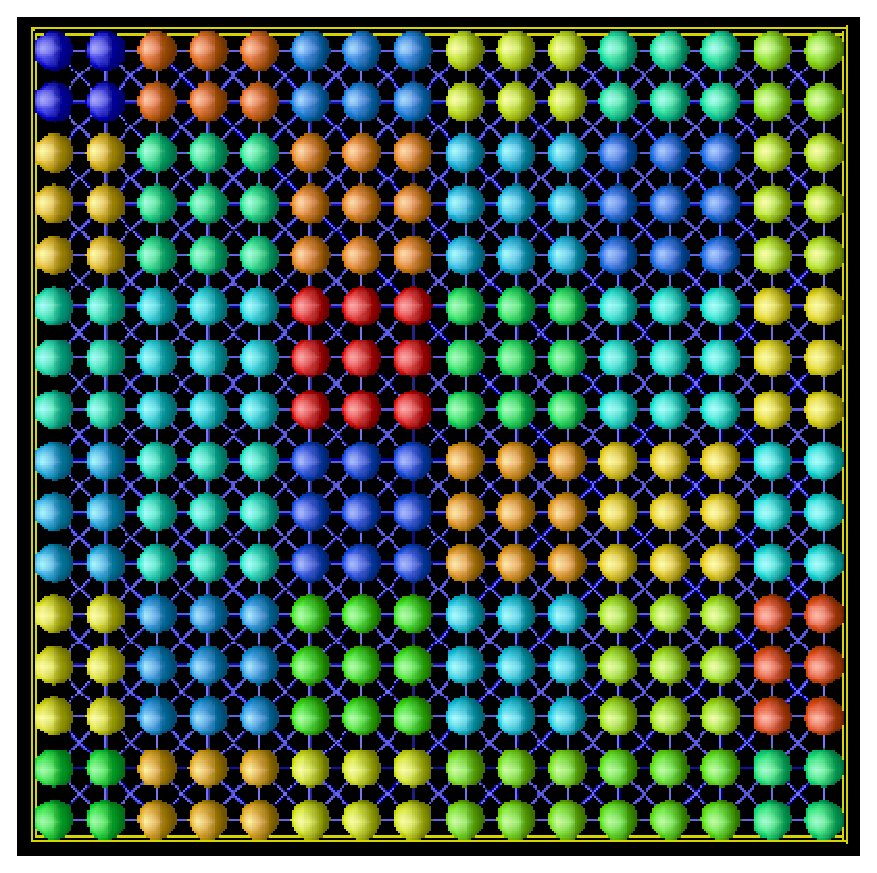
\includegraphics[height=6cm]{ml_Uncoupled-16x16.ps} \hspace{0.5cm}
  %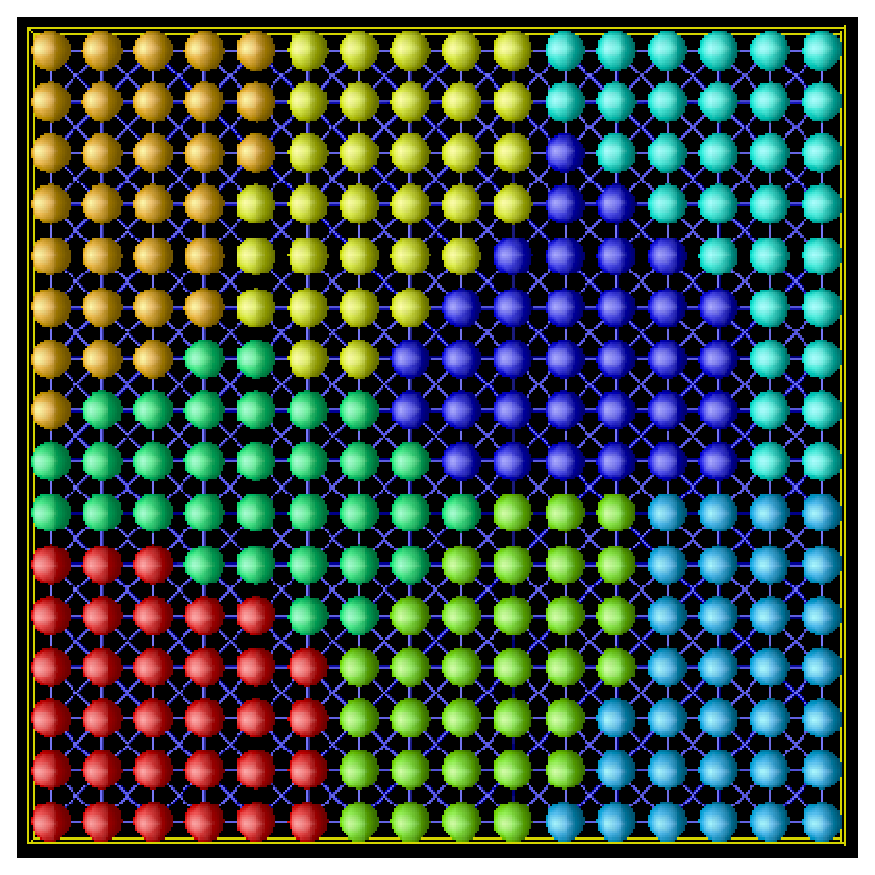
\includegraphics[height=6cm]{ml_METIS-16x16.ps}
  %\caption{Aggregates for Uncoupled (left) and METIS (right) for a 16x16 Cartesian grid.}
  %\label{fig:ml:comparison}
%\end{figure}

\begin{table}
\begin{center}
\begin{tabular}{ | p{5cm} | p{10cm} | }
\hline
\verb!Uncoupled! & For a $1$,$2$,or $3$ dimensional structured Cartesian grid 
                   with a $3$, $9$ or $27$ point stencil respectively,
                   construct aggregates of optimal size such that
                   each aggregate resides on one processor.\\
\verb!MIS! & Maximal independent set based coarsening with aggregates
             allowed to reside on multiple processes. 
             The scheme minimizes the number of iterations,
             but the cost per iteration is high.  \\
\verb!METIS! & Use a serial graph partitioner to create
               aggregates residing on one processor. 
               The number of nodes in each aggregate
               is specified with the option {\tt aggregation: nodes per aggregate}.
               ML must be configured with {\tt --with-ml\_metis}. \\
\verb!ParMETIS! & Use a parallel graph partitioner to create aggregates that
                  may reside on multiple processors.  
                  ML must be configured with {\tt --with-ml\_parmetis3x}. 
                  The number of aggregates is
                  specified by option {\tt aggregation: global number}. \\
\hline
\end{tabular}
\caption{ML\_Epetra::MultiLevelPreconditioner Coarsening Schemes}
\label{tab:ml:aggr}
\end{center}
\end{table}

\begin{table}
\begin{center}
\begin{tabular}{ | p{5cm} | p{10cm} | }
\hline
\verb!Jacobi! & Point-Jacobi. Damping factor is specified using
{\tt smoother: damping factor}, and the number of sweeps with {\tt
  smoother: sweeps} \\ 
\verb!Gauss-Seidel! & Point Gauss-Seidel. \\
\verb!Aztec! & Use AztecOO's built-in preconditioning functions as
smoothers. Or, use approximate solutions with AztecOO as smoothers. 
The AztecOO vectors \verb!options! and {\tt params} can be set using
{\tt smoother: Aztec options} and {\tt smoother: Aztec params}. \\
\hline
\end{tabular}
\caption{ML\_Epetra::MultiLevelPreconditioner Smoothers} 
\label{tab:ml:smoother}
\end{center}
\end{table}

\begin{table}
\begin{center}
\begin{tabular}{ | p{5cm} | p{10cm} | }
\hline
\verb!Jacobi! & Use Jacobi as a solver. \\
\verb!Gauss-Seidel! & Use Gauss-Seidel as a solver. \\
\verb!Amesos_KLU! & Use Amesos's KLU sequential solver. \\
\verb!Amesos_UMFPACK! & Use UMFPACK. \\
\verb!Amesos_Superludist! & Use SuperLU\_DIST. \\
\verb!Amesos_MUMPS! & Use MUMPS. \\
\hline
\end{tabular}
\caption{ML\_Epetra::MultiLevelPreconditioner Coarsest Grid Exact Solvers
  To use Amesos, ML must be configured with {\tt --enable-amesos} 
  and Amesos also be configured as needed.}
\label{tab:ml:coarse}
\end{center}
\end{table}

A very simple fragment of code using this class is reported below.
The reader may refer to file
\verb!$ML_HOME/examples/ml_example_MultiLevelPreconditioner.cpp! for a more
complex example. To run example, first 
configure ML \verb!--enable-triutils!.
\begin{verbatim}
#include "ml_include.h"
#include "ml_MultiLevelPreconditioner.h"
#include "Teuchos_ParameterList.hpp"

...

  // A is an Epetra_RowMatrix derived class object
  // solver is an AztecOO object

  Teuchos::ParameterList MList;

  // default values for smoothed aggregation
  ML_Epetra::SetDefaults("SA",MLList);
  MLList.set("max levels",6);
  MLList.set("increasing or decreasing","decreasing");
  MLList.set("aggregation: type", "MIS");
  MLList.set("coarse: type","Amesos_KLU");
  
  ML_Epetra::MultiLevelPreconditioner * MLPrec = 
    new ML_Epetra::MultiLevelPreconditioner(A, MLList, true);

  solver.SetPrecOperator(MLPrec);
  solver.SetAztecOption(AZ_solver, AZ_gmres);
  solver.Iterate(Niters, 1e-12);

  ...

  delete MLPrec;
\end{verbatim}
The general procedure is as follows. First, the user defines a Teuchos
parameters' list. Second input parameters are set via method
\verb!set(ParameterName,ParameterValue)!, where \verb!ParameterName! is
a string defining the parameter, and \verb!ParameterValue! is the
specified parameter, that can be any C++ object or pointer.  This list
is passed to the constructor, together with a pointer to the matrix, and
a boolean flag.  If this flag is set to \verb!false!, the constructor
will not compute the multilevel hierarchy until when
{\tt MLPrec->ComputePrecon-}\newline {\tt ditioner()} is called. The hierarchy can be
destroyed using \verb!MLPrec->Destroy()!.  For instance, the user may
define a code like:
\begin{verbatim}
  // A is still not filled with numerical values
  ML_Epetra::MultiLevelPreconditioner * MLPrec = 
    new ML_Epetra::MultiLevelPreconditioner(A, MLList, false);
  
  // compute the elements of A
  ...
  // now compute the preconditioner
  MLPrec->ComputePreconditioner();

  // solve the linear system, and refill A
  ...
  MLPrec->Destroy(); // destroy previous preconditioner,
  MLPrec->ComputePreconditioner(); // and build a new one
\end{verbatim}
In this fragment of code, the user defines the ML preconditioner, but
does not create the preconditioner in the construction phase. This is of
particular interest, for example, when ML is used in conjunction with
nonlinear solvers (like NOX~\cite{NOX-home-page}).

We point out that the input parameter list is {\sl copied} in the
construction phase, hence later changes to \verb!MLList! will not affect
the preconditioner. Should one need to modify parameters in the
\verb!MLPrec!'s internally stored parameter list, proceed as
follows:
\begin{verbatim}
  ParameterList & List = MLPrec->GetList();
\end{verbatim}
and then directly modify \verb!List!.

\medskip

All ML options can have a common prefix, specified by the
user in the construction phase. For example, suppose that we require
\verb!ML: ! to be the prefix. The constructor will be
\begin{verbatim}
  MLLIst.set("ML: aggregation: type", "METIS");
  ML_Epetra::MultiLevelPreconditioner * MLPrec = 
  new ML_Epetra::MultiLevelPreconditioner(*A,  
                                          MLList, 
                                          true, 
                                          Prefix);
\end{verbatim}
where \verb!Prefix! is a char array containing \verb!ML: !.

Note that spaces are important: Do not include leading or trailing
spaces, and separate words by just one space! Misspelled parameters will
not be used, and can be detected calling method \verb!PrintUnused()!
{\sl after} the construction of the multilevel hierarchy. 

For a detailed list of all the parameters, we refer to the ML user's
guide.  Here, we report the most used parameters in
Tables~\ref{tab:ml:aggr}, \ref{tab:ml:smoother} and \ref{tab:ml:coarse}.


%%%
%%%
%%%


\section{Two-Level Domain Decomposition Preconditioners with ML}
\label{sec:ml_DD}

The idea of two level domain decomposition based on aggregation is to
use a graph partitioner to partition the local or global graph into
subgraphs, and then treat each subgraph as a large aggregate.

The example contained herein 
uses the graph decomposition library METIS to create the coarse-level matrix.
If you don't have METIS, or just do not want to
re-configure ML, you may run the example 
you will be limited to use only one aggregate per process.
There are three changes to the Trilinos configuration.
One flag tells the package (ML) to look for an external library,
and the other two flag tells the compiler
where to find the include directories and external library.
Configure ML with the flags \verb!--with-ml_metis!,
and with {\tt --with-incdirs} and {\tt --with-ldflags}
set to the locations of the METIS include files and library. 
Please type {\tt configure --help} in the ML subdirectory for more information. 

Two-level domain decomposition methods are
effective for the iterative solution of many different kinds of linear
systems.  For some classes of problems, a very convenient way to define
the coarse grid operator is to use an aggregation procedure. This is very
close to what presented in Section~\ref{sec:ml_prec}. The main
difference is that only two level methods are considered, and that the
coarse grid remains of (relatively) small size. The idea is to define a
small number of aggregates on each process, using a graph decomposition
algorithm (as implemented in the library METIS, for
instance)\footnote{Aggregation schemes based on ParMETIS are also
available. Please refer to the help of the ML {\tt configure} for more
details.}. This can be done as follows.

The linear system matrix \verb!A!, here coded as an
Epetra\_CrsMatrix\footnote{Epetra\_VbrMatrix and Epetra\_RowMatrix can
  be used as well.}, corresponds to the descretization of a 2D Laplacian
on a Cartesian grid. \verb!x! and \verb!b! are the solution vector and
the right-hand side, respectively.

The AztecOO linear problem is defined as
\begin{verbatim}
  Epetra_LinearProblem problem(&A, &x, &b);
  AztecOO solver(problem);
\end{verbatim}

At this point, we can create the Teuchos parameters' list, with the
following parameters:
\begin{verbatim}
  ParameterList MLList;

  ML_Epetra::SetDefaults("DD",MLList);

  MLList.set("max levels",2);
  MLList.set("increasing or decreasing","increasing");

  MLList.set("aggregation: type", "METIS");
  MLList.set("aggregation: nodes per aggregate", 16);
  MLList.set("smoother: pre or post", "both");
  MLList.set("coarse: type","Amesos_KLU");
  MLList.set("smoother: type", "Aztec");
\end{verbatim}
The last option tells ML to use the Aztec preconditioning function as a
smoother. Aztec requires an integer vector \verb!options! and a double
vector \verb!params!. Those can be defined as follows:
\begin{verbatim}
  int options[AZ_OPTIONS_SIZE];
  double params[AZ_PARAMS_SIZE];
  AZ_defaults(options,params);
  options[AZ_precond] = AZ_dom_decomp;
  options[AZ_subdomain_solve] = AZ_icc;
  MLList.set("smoother: aztec options", options);
  MLList.set("smoother: aztec params", params);
\end{verbatim}
Note that {\sl all} Aztec preconditioners can be used as smoothers for
ML. 
At this point we can create the ML preconditioner as
\begin{verbatim}
  ML_Epetra::MultiLevelPreconditioner * MLPrec =
    new ML_Epetra::MultiLevelPreconditioner(A, MLList, true);
\end{verbatim}
and check that no options have been misspelled, using
\begin{verbatim}
  MLPrec->PrintUnused();
\end{verbatim}
AztecOO solver is called using
\begin{verbatim}
  solver.SetPrecOperator(MLPrec);

  solver.SetAztecOption(AZ_solver, AZ_cg_condnum);

  int Niters = 500;
  solver.SetAztecOption(AZ_kspace, 160);

  solver.Iterate(Niters, 1e-12);
\end{verbatim}
Finally, some (limited) information about the preconditioning phase are
obtained using
\begin{verbatim}
  cout << MLPrec->GetOutputList();
\end{verbatim}
The entire code is reported in 
\newline
\TriExe{ml/ex2.cpp}.
\newline


\clearpage
\newpage
% @HEADER
% ***********************************************************************
% 
%            Trilinos: An Object-Oriented Solver Framework
%                 Copyright (2001) Sandia Corporation
% 
% Under terms of Contract DE-AC04-94AL85000, there is a non-exclusive
% license for use of this work by or on behalf of the U.S. Government.
% 
% This library is free software; you can redistribute it and/or modify
% it under the terms of the GNU Lesser General Public License as
% published by the Free Software Foundation; either version 2.1 of the
% License, or (at your option) any later version.
%  
% This library is distributed in the hope that it will be useful, but
% WITHOUT ANY WARRANTY; without even the implied warranty of
% MERCHANTABILITY or FITNESS FOR A PARTICULAR PURPOSE.  See the GNU
% Lesser General Public License for more details.
%  
% You should have received a copy of the GNU Lesser General Public
% License along with this library; if not, write to the Free Software
% Foundation, Inc., 59 Temple Place, Suite 330, Boston, MA 02111-1307
% USA
% Questions? Contact Michael A. Heroux (maherou@sandia.gov) 
% 
% ***********************************************************************
% @HEADER

\section{Interfacing Direct Solvers with Amesos}
\label{chap:amesos}

The Amesos package provides an object-oriented interface to several
direct sparse solvers. Amesos will solve (using a direct factorization
method) the linear systems of equations (\ref{eq:linear_sys}) where $A$
is stored as an Epetra\_RowMatrix object, and $X$ and $B$ are
Epetra\_MultiVector objects.

The Amesos package has been designed to face some of the challenges of
direct solution of linear systems. In fact, many solvers have been
proposed in the last years, and often each of them requires different
input formats for the linear system matrix. Moreover, it is not uncommon
that the interface changes between revisions. Amesos aims to solve those
problems, furnishing a clean, consistent interface to many direct
solvers.

Using Amesos, users can interface their codes with a (large) variety of
direct linear solvers, sequential or parallel, simply by a code
instruction of type
\begin{verbatim}
AmesosProblem.Solver();
\end{verbatim}
Amesos will take care of redistributing data among the processors, if
necessary.

Amesos contains several classes: 
\begin{itemize}
\item \verb!Amesos_KLU!: Interface to Amesos's internal solver
  KLU~\cite{KLU};
\item \verb!Amesos_Umfpack!: Interface to Tim Davis's
  UMFPACK~\cite{umfpack-home-page};
  functionalities of this class.
\item \verb!Amesos_Dscpack!: Interface to Padma Raghavan's
  DSCPACK~\cite{dscpack-home-page};
\item \verb!Amesos_Superludist!: Interface to Xiaoye S.~Li's SuperLU
  solver suite, including SuperLU, SuperLU\_DIST 1.0 and SuperLU\_DIST
  2.0~\cite{superlu-home-page};
  presented in Section~\ref{sec:superludist}.
\item \verb!Amesos_Mumps!: Interface to MUMPS 4.3.1~\cite{mumps-home-page};
\item \verb!Amesos_Scalapack!: Interface to ScaLAPACK~\cite{scalapack}.
\end{itemize}


Note that Amesos does {\sl not} contain interfaces to LAPACK routines.
Other Trilinos packages already offer those routines (Epetra and
Teuchos).

All the Amesos classes are derived from a base class mode,
\verb!Amesos_BaseSolver!. This abstract interface provides the basic
functionalities for all Amesos solvers, and allows users to choose
different direct solvers very easily -- by changing an input scalar
parameter. See Section~\ref{sec:amesos_generic} for more details.

In this Chapter, we will suppose that matrix $A$ in
equation~(\ref{eq:linear_sys}) is defined as an Epetra\_RowMatrix, in
principle with nonzero entries on all the processes defined in the
Epetra\_Comm communicator in use. $X$ and $B$, instead, are
Epetra\_MultiVector, defined on the same communicator.  Some of the
supported packages are serial solvers: in this case, if solving with
more than one processor, the linear problem is shipped to processor 0,
solved, then the solution is broadcasted in the solution vector $X$. For
parallel solvers, instead, various options are supported, depending on
the package at hand:
\begin{itemize}
\item The Amesos\_Superludist interface can be used over all the
  processes, as well as on a subset of them. The matrix is kept in
  distributed form over the processes of interest;
\item Amesos\_Mumps can keep the matrix in a distributed form over all
  the processes, or the matrix can be shipped to processor 0. In both
  cases, all the processes in the MPI communicator will be used.
\end{itemize}

This Chapter, we will cover:
\begin{itemize}
\item The installation of the third-part packages required by Amesos, in
  Section~\ref{sec:3pl};
\item The Amesos\_BaseSolver interface to various direct solvers,
  presented (in Section~\ref{sec:amesos_generic}).
\end{itemize}

%%%
%%%
%%%

\subsection{Installation of Third-Party Packages}
\label{sec:3pl}

Amesos is an interface to other packages, mainly developed outside the
Trilinos framework\footnote{Currently, SuperLU is included in the
  Trilinos framework.}. In order to use those packages, the user should
carefully check copyright and licensing of those third party codes.
Please refer to the web page or the documentation of each particular
package for details.

Amesos supports a variety of direct solvers for linear systems of
equations, and you are likely to use Amesos with only few of them. We
suggest to define the shell variable \verb!TRILINOS_3PL!  to define the
directory used to stored third-part packages. For instance, under BASH,
you may have a line of type
\begin{verbatim}
export TRILINOS_3PL=/home/msala/Trilinos3PL
\end{verbatim}
in your \verb!.bashrc! file. Then, you may decide to create a directory
to hold include files and libraries. For instance, to compile under
LINUX with MPI:
\begin{verbatim}
$ mkdir ${TRILINOS_3PL}/LINUX_MPI
$ mkdir ${TRILINOS_3PL}/LINUX_MPI/include
$ mkdir ${TRILINOS_3PL}/LINUX_MPI/lib
\end{verbatim}
(Note that this will reflect the directory structure used by Trilinos,
see Section~\ref{sec:installing}.) While installing a package, you can
now copy all include files and libraries in these directories.

Using this setting, you can configure Amesos with a command of type
\begin{verbatim}
$ cd ${TRILINOS_HOME}/packages/amesos
$ ./configure --prefix=${TRILINOS_HOME}/LINUX_MPI \
  --enable-mpi --with-mpi-compilers \
  --enable-amesos-umfpack \
  --enable-amesos-superludist \
  --with-amesos-superludistlib=\
  "${TRILINOS_3PL}/SuperLU_DIST_2.0/libsuperlu_LINUX.a"
\end{verbatim}
(This command is followed by \verb!make! and \verb!make install!, as
usual.)  This will enable UMFPACK and SuperLU\_DIST.

For more details about the configuration options of Amesos, please refer
to Amesos documentation.

%%%
%%%
%%%



%%%
%%%
%%%

\subsection{Amesos\_BaseSolver: A Generic Interface to Direct Solvers}
\label{sec:amesos_generic}

All Amesos objects are constructed from the function class
\verb!Amesos_Factory!.  Amesos\_Factory allows a code to delay the
decision about which concrete class to use to implement the
Amesos\_BaseSolver interface. The main goal of this class is to allow
the user to select any supported (and enabled at configuration time)
direct solver, simply changing an input parameter. Another remarkable
advantage of Amesos\_BaseSolver is that, using this class, users does
not have to include the header files of the 3-part libraries in their
code\footnote{Using Amesos\_BaseSolver, 3-part libraries header files
  are required in the compilation of Amesos only.}.

An example of use of this class is as follows. First, the following
header files must be included:
\begin{verbatim}
  #include "Amesos_Factory.h" 
  #include "AmesosClassType.h"
\end{verbatim}
Then, let \verb!A! be an Epetra\_RowMatrix object (for instance, and
Epetra\_CrsMatrix). We need to define a linear problem,
\begin{verbatim}
  Epetra_LinearProblem * Amesos_LinearProblem = 
                         new Epetra_LinearProblem;
  Amesos_LinearProblem->SetOperator( A ) ; 
\end{verbatim}
and to create an Amesos parameter list (which can be empty):
\begin{verbatim}
  Teuchos::ParameterList ParamList ;
\end{verbatim}
Now, let \verb!Choice! be an AmesosClassType variable, with one of the
following values: 
\begin{itemize}
\item AMESOS\_KLU;
\item AMESOS\_UMFPACK;
\item AMESOS\_MUMPS;
\item AMESOS\_SUPERLUDIST;
\item AMESOS\_DSCPACK.
\end{itemize}
We can construct an \verb!Amesos_BaseSolver! object as follows:
\begin{verbatim}
  Amesos_BaseSolver * A_Base;
  Amesos_Factory A_Factory;

  A_Base = A_Factory.Create(Choice, *Amesos_LinearProblem, 
                            ParamList );
  assert(A_Base!=0);
\end{verbatim}
Symbolic and numeric factorizations are computed using methods
\begin{verbatim}
  A_Base->SymbolicFactorization();
  A_Base->NumericFactorization();
\end{verbatim}
The numeric factorization phase will check whether a symbolic
factorization exists or not. If not, method
\verb!SymbolicFactorization()! is invoked.  Solution is computed (after
setting of LHS and RHS in the linear problem), using
\begin{verbatim}
  A_Base->Solve();
\end{verbatim}
The solution phase will check whether a numeric factorization exists or
not. If not, method \verb!SymbolicFactorization()! is called.

Users must provide the nonzero structure of the matrix for the symbolic
phase, and the actual nonzero values for the numeric
factorization. Right-hand side and solution vectors must be set before
the solution phase, for instance using
\begin{verbatim}
  Amesos_LinearProblem->SetLHS(x);
  Amesos_LinearProblem->SetRHS(b);
\end{verbatim}

A common ingredient to all the Amesos classes is the Teuchos parameters'
list. This object, whose definition requires the input file
\verb!Teuchos_ParameterList.hpp!, is used to specify the parameters that
affect the 3-part libraries. For a detailed presentation of Teuchos, we
refer to~\cite{Teuchos-home-page}. Here, we simply recall that the
parameters' list can be created as
\begin{verbatim}
  Teuchos::ParameterList AmesosList;
\end{verbatim}
and parameters can be set as
\begin{verbatim}
  AmesosList.setParameter(ParameterName,ParameterValue);
\end{verbatim}
Here, \verb!ParameterName! is a string containing the parameter name,
and \verb!ParameterValue! is any valid C++ object that specifies the
parameter value (for instance, an integer, a pointer to an array or to
an object).

Amesos has to level of parameters: 
\begin{enumerate}
\item a first level refers to parameters that affect all solvers;
\item a second level refers to parameters that are specific to a
  particular solver.
\end{enumerate}


For a detailed list of parameters we refer to the Amesos documentation.


%\clearpage
%\newpage
%%@HEADER
% ************************************************************************
% 
%          Trilinos: An Object-Oriented Solver Framework
%              Copyright (2001) Sandia Corporation
% 
% Under terms of Contract DE-AC04-94AL85000, there is a non-exclusive
% license for use of this work by or on behalf of the U.S. Government.
% 
% This program is free software; you can redistribute it and/or modify
% it under the terms of the GNU General Public License as published by
% the Free Software Foundation; either version 2, or (at your option)
% any later version.
%   
% This program is distributed in the hope that it will be useful, but
% WITHOUT ANY WARRANTY; without even the implied warranty of
% MERCHANTABILITY or FITNESS FOR A PARTICULAR PURPOSE.  See the GNU
% General Public License for more details.
%   
% You should have received a copy of the GNU General Public License
% along with this program; if not, write to the Free Software
% Foundation, Inc., 675 Mass Ave, Cambridge, MA 02139, USA.
% 
% Questions? Contact Michael A. Heroux (maherou@sandia.gov)
% 
% ************************************************************************
%@HEADER

\section{Eigenvalue and Eigenvector Computations with Anasazi}
\label{chap:anasazi}

The Anasazi package was designed as an extensible and interoperable framework
for large-scale eigenvalue algorithms. Anasazi provides a generic interface to a
collection of algorithms for solving large-scale eigenvalue problems. It
utilizes interfaces for operators and multivectors, and therefore it can be used
with any operator or multivector class that implements these interfaces. The
algorithms currently available through Anasazi are a block Krylov Schur method,
a block Davidson method and the locally optimal block preconditioned conjugate
gradient (LOBPCG) method.

In this Chapter we present:
\begin{itemize}
\item a description of the Anasazi framework (Section~\ref{sec:anasazi:framework}),
\item the interface to the Epetra linear algebra package
(Section~\ref{sec:anasazi:epetra}), and
\item an example using Anasazi for the solution of an eigenvalue problem 
(Section~\ref{sec:anasazi:example}).
\end{itemize}


Throughout this chapter, the following abbreviations may be used for the sake of
brevity:
\begin{itemize}
\item ST - scalar type class
\item MV - multivector type class
\item OP - operator type class
\end{itemize}

%%%
%%%
%%%
\subsection{Anasazi Framework}
\label{sec:anasazi:framework}

Solving an eigenproblem in Anasazi requires the use of four main entities: an
eigenvalue problem, an eigenvalue solver, linear operators and multivectors. The
representations of these objects are described by the following four Anasazi
classes:
\begin{itemize}
\item \verb!Eigenproblem! (Section~\ref{sec:anasazi:eigenproblem}) - this class defines the interface required by an
eigensolver to solve an eigenvalue problem.
\item \verb!Eigensolver! (Section~\ref{sec:anasazi:eigensolver}) - this class defines the basic interface that any
eigensolver must support.
\item \verb!MultiVecTraits! (Section~\ref{sec:anasazi:mvt}) - this class defines the interface Anasazi uses to 
perform operations on and with multivectors.
\item \verb!OperatorTraits! (Section~\ref{sec:anasazi:opt}) - this class defines the interface by which Anasazi
applies operators to multivectors.
\end{itemize}

While the four classes listed above are the most important, there are other
classes that are necessary when using Anasazi. These include the
\verb!SortManager!, \verb!OutputManager! and \verb!ModalSolverUtils! classes.
These classes, along with the four classes introduced above, are described in
more detail in the following subsections.

%%%
%%%
\subsubsection{Anasazi::Eigenproblem}
\label{sec:anasazi:eigenproblem}

One of the goals of Anasazi is to provide a framework for eigenvalue
computations that leaves as much flexibility to the user as possible. It is
towards this goal that the \verb!Anasazi::Eigenproblem! abstract base class was
defined. By providing a base class for an eigenvalue problem which the user can
extend, Anasazi allows the user to specify properties of the eigenvalue problem,
such as the inner product and the vector norm. However, by requiring
eigenproblems to derive from \verb!Anasazi::Eigenproblem!, Anasazi defines a
minimum interface that can be expected of all eigenvalue problems by the classes
that will work with the problems (i.e., eigensolvers and status testers).

Both the eigenproblem and the eigensolver in Anasazi are templated according
to the scalar type, the multivector type and the operator type. Before
declaring an eigenproblem, the user must choose classes to represent these
entities. Having done so, the user can begin to specify the parameters of the
eigenvalue problem. The \verb!Anasazi::Eigenproblem! defines \textbf{set} methods for
the parameters of the eigenproblem. These methods are:
\begin{itemize}
\item \verb!SetOperator! - set the operator for which the eigenvalues will be computed
\item \verb!SetA! - set the $A$ operator for the eigenvalue problem $Ax=\lambda M x$
\item \verb!SetM! - set the $M$ operator for the eigenvalue problem $Ax=\lambda M x$
\item \verb!SetPrec! - set the preconditioner for the eigenvalue problem
\item \verb!SetInitVec! - set the initial guess
\item \verb!SetAuxVec! - set the auxilliary vectors
\item \verb!SetNEV! - set the number of eigenvalues to be computed
\item \verb!SetSymmetric! - set the symmetry of the problem
\end{itemize}
In addition to these \textbf{set} methods, \verb!Anasazi::Eigenproblem! defines
a method \verb!SetProblem()! which gives the class the opportunity to perform any
initialization that may be necessary before the problem is handed off to an
eigensolver.

For each of the \textbf{set} methods listed above, there is a corresponding
\textbf{get} function. These are the functions used by the eigensolver to get
the necessary information from the eigenvalue problem. In addition, there are
two methods for returning the results of the eigenvalue computation:
\begin{verbatim}
Teuchos::RefCountPtr< MV > GetEvals()
Teuchos::RefCountPtr< std::vector< ScalarType > > GetEvecs()
\end{verbatim}

In this regard, the eigenproblem acts as a repository for information about the
eigenvalue problem. However, this is not the only function of the
\verb!Anasazi::Eigenproblem! class. The class also provides two functions,
\verb!InnerProd! and \verb!MvNorm!, which specify the inner product and the
vector norm to be used when computing the solution of the eigenvalue problem.
When creating a concrete derived class of \verb!Anasazi::Eigenproblem!, the
developer can choose to implement these methods as she prefers.

Anasazi provides users with an implementation of \verb!Anasazi::Eigenproblem!,
called \verb!Anasazi::BasicEigenproblem!.  The inner product implemented by this
class is the $M$-inner product or the standard Euclidean inner product if $M$ is
not specified. The vector norm implemented by this class is the norm induced by
the inner product.  This formulation provides all the functionality necessary to
describe both generalized and standard linear eigenvalue problems. The user may
wish to create her own derivation of \verb!Anasazi::Eigenproblem! if she desires
a different inner product or is solving an eigenvalue problem not described by
\verb!Anasazi::BasicEigenproblem! (e.g. a quadratic eigenvalue problem).

An example for declaring an eigenvalue problem using
\verb!Anasazi::BasicEigenproblem! is given in Section~\ref{sec:anasazi:example}.

%%%
%%%
\subsubsection{Anasazi::Eigensolver}
\label{sec:anasazi:eigensolver}

The \verb!Anasazi::Eigensolver! class defines the basic interface that must be
met by an eigensolver class in Anasazi. The specific eigensolvers are impelented
as derived classes of \verb!Anasazi::Eigensolver!.
Table~\ref{tab:anasazi:solvers} lists the eigensolver currently implemented in
Anasazi.

\begin{table}[htp]
\begin{center}
\begin{tabular}{| p{4cm} p{8cm} |}
\hline
Solver & Description \\
\hline
{\tt BlockDavidson}    & A block Davidson solver for symmetric
                         eigenvalue problems.\\
{\tt BlockKrylovSchur} & A block Krylov Schur solver for symmetric or
                         nonsymmetric problems.\\
{\tt LOBPCG} & The locally optimal block preconditioned conjugate gradient
method.\\
\hline
\end{tabular}
\caption{Eigensolvers currently implemented in Anasazi.}
\label{tab:anasazi:solvers}
\end{center}
\end{table}

The class \verb!Anasazi::Eigensolver!, like \verb!Anasazi:Eigenproblem!, is
templated according the scalar type, the multivector type and the operator
type. The procedure for using an Anasazi eigensolver is as follows:
\begin{enumerate}
\item Choose scalar, multivector and operator classes.
\item Create the eigenproblem.
\item Create an instance of the desired eigensolver and pass it the necessary
options.
\item Ask the eigensolver to solve the eigenproblem.
\end{enumerate}

The options for the eigensolver are passed through the constructor, defined by
\verb!Anasazi::Eigensolver! to have the following form:
\begin{verbatim}
Eigensolver( 
   const Teuchos::RefCountPtr<Eigenproblem<ScalarType,MV,OP> > &problem, 
   const Teuchos::RefCountPtr<SortManager<ScalarType,MV,OP> > &sm,
   const Teuchos::RefCountPtr<OutputManager<ScalarType> > &om,
   Teuchos::ParameterList &pl );
\end{verbatim}

The first argument is the eigenvalue problem that is to be solved. The second
option is an instance of \verb!Anasazi::SortManager!. The goal of this class is
to specify the eigenvalues targeted by the solver and to provide sorting
functionality (Section~\ref{sec:anasazi:sm}). The third parameter is an instance
of \verb!Anasazi::OutputManager!. This class specifies the verbosity of the
eigensolver and other printing options (Section~\ref{sec:anasazi:om}). The last
parameter is an instance of the class \verb!Teuchos::ParameterList!. This is the
mechanism by which solver-specific options are passed to the eigensolver (e.g.,
block size, number of restarts).  A list of valid parameters for each
eigensolver is given in Tables~\ref{tab:anasazi:bks_params},
\ref{tab:anasazi:bd_params}, and \ref{tab:anasazi:lobpcg_params}.

\begin{remark}
Anasazi makes extensive use of the Teuchos utility classes, especially
\verb!RefCountPtr! (Section~\ref{sec:teuchos:RefCountPtr}) and
\verb!ParameterList! (Section~\ref{sec:teuchos:ParameterList}). The
user is encouraged to become familiar with these classes and their correct
usage.
\end{remark}

\begin{table}
\begin{center}
\begin{tabular}{| p{4cm} l |}
\hline
Parameter & Description \\
\hline
{\tt Block Size}   & The number of vectors added to the basis at each iteration \\
{\tt Max Blocks}   & The maximum number of blocks in the Krylov basis \\
{\tt Max Restarts} & Stopping criterion on the number of restarts \\
{\tt Step Size}    & Controls the frequency of projected Schur computations \\
{\tt Tol}          & Stopping criterion on relative residual norm \\
\hline
\end{tabular}
\caption{Options for Anasazi::BlockKrylovSchur}
\label{tab:anasazi:bks_params}
\end{center}
\end{table}

\begin{table}
\begin{center}
\begin{tabular}{| p{4cm} l |}
\hline
Parameter & Description \\
\hline
{\tt Block Size} & The number of vectors added to the basis at each iteration \\
{\tt Max Blocks} & The maximum number of blocks in the Krylov basis \\
{\tt Max Iters}  & Stopping criterion on the number of iterations \\
{\tt Tol}        & Stopping criterion on relative residual norm \\
\hline
\end{tabular}
\caption{Options for Anasazi::BlockDavidson}
\label{tab:anasazi:bd_params}
\end{center}
\end{table}

\begin{table}
\begin{center}
\begin{tabular}{| p{4cm} l |}
\hline
Parameter & Description \\
\hline
{\tt Block Size} & The number of vectors added to the basis at each iteration \\
{\tt Max Iters}  & Stopping criterion on the number of iterations \\
{\tt Tol}        & Stopping criterion on relative residual norm \\
\hline
\end{tabular}
\caption{Options for Anasazi::LOBPCG}
\label{tab:anasazi:lobpcg_params}
\end{center}
\end{table}

After passing all of the options to the eigensolver, all that remains is to ask
it to solve the eigenproblem. This is done by calling the solve routine 
defined by \verb!Anasazi::Eigensolver!:
\begin{verbatim}
Anasazi::ReturnType solve()
\end{verbatim}
This function returns the status of the solver. Possible return values are
listed in Table~\ref{tab:anasazi:rt}. After calling \verb!solve()!, the
eigensolver class defines some \textbf{get} functions to retrieve information
relevant to many eigensolvers. These are:
\begin{verbatim}
int GetNumIters() const
int GetNumRestarts() const
int GetBlockSize() const 
\end{verbatim}
The class also defines a \verb!GetEigenproblem()! function, which returns a
reference to the eigenproblem the solver was working on.

\begin{table}
\begin{center}
\begin{tabular}{| p{4cm} l |}
\hline
Parameter & Default \\
\hline
Anasazi::Ok          & Success. \\
Anasazi::Unconverged & Solver did not converge to specified accuracy. \\
Anasazi::Failed      & An error with the input or in the solver. \\
\hline
\end{tabular}
\caption{Anasazi::ReturnType values.}
\label{tab:anasazi:rt}
\end{center}
\end{table}

%%%
%%%
\subsubsection{Anasazi::MultiVecTraits}
\label{sec:anasazi:mvt}

As mentioned above, the eigenproblem and eigensolver classes are templated
classes, allowing the user to specify desired classes for scalars, multivectors
and linear operators. The choice of scalar type allows Anasazi to be implemented
with arbitrary numerical precision, while the choice of multivector and operator
classes allows Anasazi to leverage the power of any existing linear algebra
libraries available to the user. This flexibility is accomplished the usage of
the \verb!Anasazi::MultiVecTraits! class. This class defines an opaque
interface, specifying the operations that the chosen multivector class must
support in order to be used by Anasazi. These methods are listed in
Table~\ref{tab:anasazi:mvt}.

\begin{table}
\begin{center}
\begin{tabular}{| p{4cm} || p{8cm} |}
\hline
Method name & Description \\
\hline\hline
Clone           & Creates a new empty multivector containing a specified number
of columns.  \\\hline
CloneCopy       & Creates a new MV with a copy of the contents of an existing
multivector (deep copy). \\\hline
CloneCopy       & Creates a new multivector with a copy of the selected contents of
an existing multivector (deep copy).  \\\hline
CloneView       & Creates a new multivector that shares the selected contents of
an existing multivector (shallow copy).  \\\hline
CloneView       & Creates a new const multivector that shares the selected
contents of an existing multivector (shallow copy).  \\\hline
GetVecLength    & Obtain the vector length of a multivector.  \\\hline
GetNumberVecs   & Obtain the number of vectors in a multivector.  \\\hline
MvTimesMatAddMv & Perform $mv \leftarrow \alpha AB + \beta mv$.  \\\hline
MvAddMv         & Perform $mv \leftarrow \alpha A + \beta B$.  \\\hline
MvTransMv       & Compute the matrix $C \leftarrow \alpha A^H B$.  \\\hline
MvDot           & Compute the vector $b$ where the components are the individual
dot-products of the $i$-th columns of $A$ and $B$, i.e. $b[i] = A[i]^H B[i]$.
\\\hline
MvNorm          & Compute the 2-norm of each individual vector of $A$.  \\\hline
SetBlock        & Copy the vectors in $A$ to a subset of vectors in $B$. \\\hline
MvRandom        & Replace the vectors in $A$ with random vectors.  \\\hline
MvInit          & Replace each element of the vectors in $A$ with $\alpha$.  \\\hline
MvPrint         & Print the multi-vector to an output stream.  \\\hline
\hline
\end{tabular}
\caption{Methods required by MultiVecTraits interface.}
\label{tab:anasazi:mvt}
\end{center}
\end{table}

For example, a user might declare an Anasazi eigensolver templated with a
multivector class \verb!MyMVClass!. In solving the eigenproblem, the solver will
manipulate multivectors using a specialization of the traits class, like
follows:
\begin{verbatim}
Anasazi::MultiVecTraits<MyMVClass>::MvRandom( A )
\end{verbatim}
If a specialization of \verb!Anasazi::MultiVecTraits! for \verb!MyMVClass! does
not exist or is not complete, then a program using this class will not compile.

In order to use Anasazi with a specific multivector class, the sole requirement
is that there is a \verb!Anasazi::MultiVecTraits! specialization for the chosen
class. There are multiple ways to satisfy this. The first approach is
to derive from a class for which a \verb!Anasazi::MultiVecTraits! specialization
already exists. Anasazi provides an abstract class for this purpose, called
\verb!Anasazi::MultiVector!. The user would define a new class which implements
all of the methods specified by \verb!Anasazi::MultiVector!. This approach is
appropriate for the user looking to develop a linear algebra code from scratch.

A second approach is to declare a specialization of
\verb!Anasazi::MultiVecTraits! for the desired multivector class. This is the
most appropriate approach for a user who already has a multivector class that
she would like to use. The user would use the \verb!Anasazi::MultiVecTraits!
interface as a wrapper around the functionality of the existing class.

Finally, for the user who does not have an existing linear algebra codes and
does not wish to implement her own multivector class, Anasazi provides an
interface to the Epetra linear algebra library. In addition to providing the
user with a parallel linear algebra class, this allows the user to utilize any
other Trilinos software that recognizes the Epetra multivector class.

\begin{remark} 
An Anasazi eigenproblem and eigensolver are templated based on a scalar type, a
multivector type, and an operator type. The scalar type have a
\verb!Teuchos::ScalarTraits! specialization, and the multivector and operator
types must have \verb!Anasazi::MultiVecTraits! and
\verb!Anasazi::OperatorTraits! specializations, respectively. This allows
Anasazi to locally specify the requirements necessary of multivector and
operator classes, without requiring the user to rewrite their classes to derive
from Anasazi base classes.
\end{remark}



%%%
%%%
\subsubsection{Anasazi::OperatorTraits}
\label{sec:anasazi:opt}

Just as \verb!Anasazi::MultiVecTraits! defined the interface required to use a
multivector class with Anasazi, \verb!Anasazi::OperatorTraits! defines the
interface required to use the combination of a specific operator class with a
specific multivector class. This interface defines a single method:
\begin{verbatim}
ReturnType Apply (const OP &Op, const MV &x, MV &y)
\end{verbatim}
This method performs the operation $y = Op*x$, where $Op$ is an operator of type
\verb!OP! and $x$ and $y$ are multivectors of type $VM$. In order to use the
combination of \verb!OP! and \verb!MV!, there must be a specialization of
\verb!Anasazi::OperatorTraits! for \verb!OP! and \verb!MV!. This can be
accomplished in a few different ways, just as described for the multivector in
the previous section:
\begin{itemize}
\item subclass the \verb!Anasazi::Operator! abstract class (templated with
\verb!MV!), for which a \verb!OperatorTraits! specialization already exists,
\item define a specialization satisfying \verb!OperatorTraits! for multivector
class \verb!MV! and operator class \verb!OP!,
\item use a \verb!Epetra_Operator!, or
for which a \verb!OperatorTraits! specialization is already defined.
\end{itemize}

The first makes sense in situations where the user is planning on writing an
operator class from scratch. The second is most appropriate when the user has an
existing operator class. The third is appropriate for a user who does not have
an existing linear algebra suite. Section~\ref{sec:anasazi:epetra} gives an
example of using the Anasazi interface to Epetra to use Epetra's multivector and
oerator classes.

%%%
%%%
\subsubsection{Anasazi::SortManager}
\label{sec:anasazi:sm}

The purpose of a sort manager is to separate the eigensolver classes from the
sorting functionality required by those classes. This satisfies the principal of
flexibility sought by Anasazi, by giving the user the opportunity to perform the
sorting in whichever manner is deemed to be most appropriate. Anasazi defines
an abstract class \verb!Anasazi::SortManager! with only two methods: one for
real and one for complex:
\begin{verbatim}
ReturnType  
   sort (..., ST *evals, std::vector<int> *perm) 
ReturnType 
   sort (..., ST *r_evals, ST *i_evals, std::vector<int> *perm)
\end{verbatim}
Each of these sort routines will sort the eigenvalues according to some
implementation, and optionally return the perumtation vector as well (useful for
sorting associated vectors).

Anasazi provides a derived class \verb!Anasazi::BasicSort! which implements
\verb!Anasazi::SortManager!. This class provides basic sorting functionality,
described in Table~\ref{tab:anasazi:sm}.

\begin{table}
\begin{center}
\begin{tabular}{| p{2cm} l |}
\hline
Option & Action \\
\hline
{\tt SM} & Sort eigenvalues in increasing order of magnitude \\
{\tt SR} & Sort eigenvalues in increasing order of real part \\
{\tt SI} & Sort eigenvalues in increasing order of imaginary part \\
{\tt LM} & Sort eigenvalues in decreasing order of magnitude \\
{\tt LR} & Sort eigenvalues in decreasing order of real part \\
{\tt LI} & Sort eigenvalues in decreasing order of imaginary part \\
\hline
\end{tabular}
\caption{Options for Anasazi::BasicSort.}
\label{tab:anasazi:sm}
\end{center}
\end{table}


%%%
%%%
\subsubsection{Anasazi::OutputManager}
\label{sec:anasazi:om}

As with the sort manager, the output manager in Anasazi exists to provide
flexibility with regard to the verbosity of the eigensolver. An instance of
\verb!Anasazi::OutputManager! is declared as followed:
\begin{verbatim}
Anasazi::OutputManager<ST> MyOM(myID, verblevel, printID, ostream);
\end{verbatim}
The parameter \verb!myID! is the ID of the current process and \verb!printID! is
designates which process should print. Parameter \verb!verbLevel! is a bitmask
specifying the desired verbosity level of the eigensolver (see
Table~\ref{tab:anasazi:om}). Lastly, \verb!ostream! is the output stream that
should be used when printing from the eigensolver.

\begin{table}
\begin{center}
\begin{tabular}{| p{7cm} l |}
\hline
Option & Action \\
\hline
{\tt Anasazi::Error} & 
  This option is always set \\
{\tt Anasazi::Warning} & 
  Warnings \\
{\tt Anasazi::IterationDetails} & 
  Details at each iteration \\
{\tt Anasazi::OrthoDetails} & 
  Details about orthogonality \\
{\tt Anasazi::FinalSummary} & 
  A final summary \\
{\tt Anasazi::Debug} & 
  Debugging information \\
\hline
\end{tabular}
\caption{Options for Anasazi::OutputManager.}
\label{tab:anasazi:om}
\end{center}
\end{table}

Inside an eigensolver, the output manager is accessed via the following
routines:
\begin{itemize}
\item \verb!GetOstream()! - returns the output stream to which messages should
be redirected.
\item \verb!isVerbosityAndPrint(type)! - decides whether messages of class
\verb!type! should be printed by this process.
\item \verb!isVerbosity(type)! - decides whether messages of class \verb!type!
should be printed at all, and therefore, whether joint computation may be
necessary.
\item \verb!doPrint()! - whether messages can be printed through the output
stream by this process.
\end{itemize}

%%%
%%%
\subsubsection{Anasazi::ModalSolverUtils}
\label{sec:anasazi:msu}

This class is the Anasazi utility class. It contains methods for
sorting/permuting vectors in a multivector, for performing orthogonalization,
for solving projected eigenvalue problems, and for doing sanity checks. A
complete description of this class is available in the Anasazi documentation.

%%%
%%%
%%%
\subsection{Using the Anasazi interface to Epetra}
\label{sec:anasazi:epetra}

The Epetra package provides the underlying foundation for all Trilinos solvers.
By using the Anasazi interface to Epetra, the user not only avoids the trouble
of designing her own multivector and operator classes, but also gains the
ability to utilize any other Trilinos package which recognizes Epetra classes
(such as AztecOO, IFPACK, and others).

In order to use the Epetra interface to Anasazi, the user must include
the following file:
\begin{verbatim}
#include "AnasaziEpetraAdapter.hpp"
\end{verbatim}
This file simply defines specializations of the \verb!Anasazi::MultiVecTraits!
and \verb!Anasazi::OperatorTraits! classes, while also including the Epetra
header files defining the multivector and operator classes.

In addition, the user will need one of the following, depending on
whether MPI is used or not:
\begin{verbatim}
#include "Epetra_MpiComm.h"
#include "Epetra_SerialComm.h"
\end{verbatim}
For more information about the \verb!Epetra_Map! and \verb!Epetra_Comm!
classes, see the tutorial section covering Epetra (Sections~\ref{sec:comm} and
\ref{sec:map}).

Because Epetra makes exclusive use of double precision arithmetic, choosing
\verb!Epetra_Operator! and \verb!Epetra_MultiVector! makes sense only for the
scalar type \verb!double!. For brevity, it is useful to declare type definitions
for these classes:
\begin{verbatim}
typedef Epetra_MultiVector MV;
typedef Epetra_Operator OP;
\end{verbatim}

Multivectors will be of type \verb!MV!:
\begin{verbatim}
Teuchos::RefCountPtr<MV> X = Teuchos::rcp( new MV(...) );
\end{verbatim}

Operators can be any subclass of \verb!OP!, for example, a \verb!Epetra_CsrMatrix!:
\begin{verbatim}
Teuchos::RefCountPtr<OP> A = Teuchos::rcp( new Epetra_CrsMatrix(...)  );
\end{verbatim}

The Anasazi interface to Epetra defines a specialization of
\verb!Anasazi::MultiVecTraits! for \verb!Epetra_MultiVector! and a
specialization of \verb!Anasazi::OperatorTraits! for \verb!Epetra_Operator!
applied to \verb!Epetra_MultiVector!. Therefore, we can now specify an
eigenproblem and eigensolver utilizing these computational classes. An example
defining an eigenvalue problem and solving the problem using an Anasazi
eigensolver is given in the next section.

%%%
%%%
%%%
\subsection{Defining and Solving an Eigenvalue Problem}
\label{sec:anasazi:example}

The first step in solving an eigenvalue problem is to define the eigenvalue
problem. Assume we have chosen classes to represent our scalars, multivectors
and operators, as \verb!ST!, \verb!MV! and \verb!OP!, respectively. Given an
operator \verb!A! and a multivector \verb!X! containing initial vectors, both
wrapped in \verb!Teuchos::RefCountPtr!s, we might define the eigenproblem as
follows:
\begin{verbatim}
Teuchos::RefCountPtr< BasicEigenproblem<ST,MV,OP> > MyProblem 
  = Teuchos::rcp( new BasicEigenproblem<ST,MV,OP>(A,X) );
MyProblem->SetSymmetric( true );
MyProblem->SetNEV( 5 );
MyProblem->SetProblem();
\end{verbatim}

The first line creates a \verb!BasicEigenproblem! object and wraps it
in a Teuchos smart-pointer. The second line specifies the symmetry of
the eigenproblem, information which may be utilized by the eigensolver
for extra efficiency. The third line specifies the desired number of
eigenvalues and eigenvectors. Lastly, the fourth signals that we have
finished setting up the eigenproblem. This step must be completed
before attempting to solve the problem.

Let us, for example, attempt to solve this eigenvalue problem with a
block Krylov Schur solver. First, we declare a sort manager to specify the
targeted eigenvalues:
\begin{verbatim}
std::string which("SM");
Teuchos::RefCountPtr<Anasazi::BasicSort<ST,MV,OP> > MySM =
  Teuchos::rcp( new Anasazi::BasicSort<ST,MV,OP>(which) );
\end{verbatim}
The option chosen was \verb!"SM"!, signaling that we want to compute
the eigenvalues with the smallest magnitude. 

Next we create an output manager, specifying the verbosity of the
solver:
\begin{verbatim}
Teuchos::RefCountPtr<Anasazi::OutputManager<ST> > MyOM = 
  Teuchos::rcp(  new Anasazi::OutputManager<ST>( MyPID ) );
MyOM->SetVerbosity( Anasazi::Error+Anasazi::Warning );
\end{verbatim}
Here, we have asked for information regarding errors and warnings from
the eigensolver.

We also will specify the parameters for the eigensolver:
\begin{verbatim}
Teuchos::ParameterList MyPL;
MyPL.set( "Block Size", 5 );
MyPL.set( "Max Blocks", 5 );
MyPL.set( "Max Restarts", 100 );
MyPL.set( "Tol", 1.0e-8 );
\end{verbatim}

We now have all of the information needed to declare the eigensolver
and solve the problem:
\begin{verbatim}
Anasazi::BlockKrylovSchur<ST,MV,OP> 
  MySolver( MyProblem, MySM, MyOM, MyPL );
\end{verbatim}
The eigenproblem is solved with the instruction
\begin{verbatim}
Anasazi::ReturnType sret = MySolver.solve();
\end{verbatim}
The return value of the solver indicates whether the algorithm
succeeded or not. 

Eigenvectors and eigenvalues can be retrieved using
\begin{verbatim}
Teuchos::RefCountPtr<Epetra_MultiVector >  evecs 
   = MyProblem->GetEvecs();
Teuchos::RefCountPtr<std::vector<double> > evals 
   = MyProblem->GetEvals();
\end{verbatim}
For a nonsymmetric problem with potentially complex eigenvalues and
eigenvectors, \verb!evecs! and \verb!evals! contain both the real and
complex parts of these, as described in the comments of
\TriExe{anasazi/ex1.cpp}.

Example \TriExe{anasazi/ex1.cpp} shows how to compute the eigenvectors
corresponding to the lowest eigenvalues for a 2D Laplace problem using the block
Krylov Schur solver.  Example \TriExe{anasazi/ex2.cpp} solves this example,
using instead the block Davidson eigensolver.  Finally, the block Krylov Schur
solver is used to solve a nonsymmetric convection-diffusion problem in Example
\TriExe{anasazi/ex3.cpp}.

%Table~\ref{tab:anasazi:exLapl} reports the lower
%eigenvalues. 

%\begin{figure}[htbp]
%  \centering
%  \includegraphics[height=6cm]{anasazi_Laplace_1D.ps}
%  \caption{Lowest eigenvalues of a 1D Laplace problem, with $h=1/33$.}
%  \label{fig:anasazi:1D}
%\end{figure}

%\begin{table}[htbp]
%  \centering
%  \begin{tabular}{| l | c |}    
%    \hline
%& {\tt laplace\_2d} \\
%     \hline
%     $h = 1/33$  & 0.00905   & 0.0181    & 0.02716  \\
%     $h = 1/65$  & 0.00235   & 0.00467   & 0.007006 \\
%     $h = 1/129$ & 0.0005936 & 0.0011861 & -        \\
%     $h = 1/257$ & 0.000149  & 0.0002983 & -        \\
%     $h = 1/513$ & 3.75e-5   & -         & -        \\
%     \hline
%  \end{tabular}
%  \caption{$\lambda_{min}$ for 1D, 2D and 3D Laplace problem on a Cartesian mesh.}
%  \label{tab:anasazi:exLapl}
%\end{table}
%%%
%%%
%%%



% FIXME
%\subsection{Concluding Remarks on Anasazi}
%\label{sec:anasazi_concluding}

%More documentation on the Anasazi package can be found in
%\cite{Anasazi-Ref-Guide,Anasazi-User-Guide}.



\clearpage
\newpage
% @HEADER
% ***********************************************************************
% 
%            Trilinos: An Object-Oriented Solver Framework
%                 Copyright (2001) Sandia Corporation
% 
% Under terms of Contract DE-AC04-94AL85000, there is a non-exclusive
% license for use of this work by or on behalf of the U.S. Government.
% 
% This library is free software; you can redistribute it and/or modify
% it under the terms of the GNU Lesser General Public License as
% published by the Free Software Foundation; either version 2.1 of the
% License, or (at your option) any later version.
%  
% This library is distributed in the hope that it will be useful, but
% WITHOUT ANY WARRANTY; without even the implied warranty of
% MERCHANTABILITY or FITNESS FOR A PARTICULAR PURPOSE.  See the GNU
% Lesser General Public License for more details.
%  
% You should have received a copy of the GNU Lesser General Public
% License along with this library; if not, write to the Free Software
% Foundation, Inc., 51 Franklin St, Fifth Floor, Boston, MA 02110-1301
% USA
% Questions? Contact Michael A. Heroux (maherou@sandia.gov) 
% 
% ***********************************************************************
% @HEADER

\chapter{Solving Nonlinear Systems with NOX}
\label{chap:nox}

\ChapterAuthors{Marzio Sala, Michael Heroux, David Day}

\begin{introchapter}
NOX is a suite of solution methods for the solution of nonlinear
systems of type
\begin{equation}
\label{eq:nonlinear}
F(x) = 0,
\end{equation}
where
\[
F(x) = 
\begin{pmatrix}
  f_1(x_1, \ldots, x_n) \\
  \vdots \\
  f_n(x_1, \ldots, x_n) \\
\end{pmatrix}
\]
is a nonlinear vector function, and the Jacobian matrix of $F$, $J$, is
defined by
\[
J_{i,j} = \frac{ \partial F_i}{\partial x_j} (x).
\]

NOX aims to solver (\ref{eq:nonlinear}) using Newton-type methods. NOX
uses an abstract vector and ``group'' interface. Current implementation
are provided for Epetra/AztecOO objects, but also for LAPACK and PETSc.
It provides various strategies for the solution of nonlinear systems,
and it has been designed to be easily integrated into existing
applications.

In this Chapter, we will
\begin{itemize}
\item Outline the basic issue of the  solution of nonlinear
  systems (in Section~\ref{sec:nox_theoretical});
\item Introduce the NOX package (in Section \ref{sec:nox_intro});
\item Describe how to introduce a NOX solver in an existing code (in
  Section \ref{sec:nox_introduce});
\item Present Jacobian-free methods (in
  Section~\ref{sec:nox_jacobian_free}).
\end{itemize}
\end{introchapter}

%%%
%%%
%%%

\section{Theoretical Background}
\label{sec:nox_theoretical}

Aim of this Section is to briefly present some aspects of the solution
of nonlinear systems, to establish a notation. The Section is not
supposed to be exhaustive, nor complete on this subject. The reader is
referred to the existing literature for a rigorous presentation.

\medskip

To solve system of nonlinear equations, NOX makes use of Newton-like methods.
The Newton method defines a suite $\{ x_k\}$ that, under some
conditions, converges to $x$, solution of~(\ref{eq:nonlinear}).
The algorithm is as follows: given $x_0$, for $k=1,\ldots$ until
convergence, solve
\begin{equation}
J_k  (x_{k-1})\left ( x_{k} - x_{k-1} \right) = 
- F(x_{k-1}),\quad
J_k  (x_{k-1}) =  \left[ \frac{ \partial F}{
        \partial x}( x_{k-1}) \right] .
\label{eq:newton_step}
\end{equation}
Newton method introduces a local full linearizion of the equations.
Solving a system of linear equations at each Newton step can be very
expensive if the number of unknowns is large, and may not be justified
if the current iterate is far from the solution. Therefore, a departure
from the Newton framework consists of considering {\em inexact} Newton
methods, which solve system~(\ref{eq:newton_step}) only approximatively.

In fact, in practical implementation of the Newton method, one or more
of the following approximations are used:
\begin{enumerate}
\item The Fr\'echet derivative $J_k$ for the Newton step is not
  recomputed at every Newton step;
\item The equation for the Newton step~(\ref{eq:newton_step}) is solved
  only inexactly;
\item Defect-correction methods are employed, that is, $J_k$ is
  numerically computed using low-order (in space) schemes, while the
  right-hand side is built up using high-order methods.
\end{enumerate}

For a given initial guess, ``close enough'' to the solution of
(\ref{eq:nonlinear}), the Newton method with exact linear solves
converges quadratically. In practice, the radius of convergence is often
extended via various methods. NOX provides, among others, line search
techniques and trust region strategies.

%%%
%%%
%%%

\section{Creating NOX Vectors and Group}
\label{sec:nox_intro}

NOX is not based on any particular linear algebra package. Users are
required to supply methods that derive from the abstract classes
\verb!NOX::Abstract::Vector! (which provides support for basic vector
operations as dot products), and \verb!NOX::Abstract::Group!  (which
supports the linear algebra functionalities, evaluation of the function
$G$ and, optionally, of the Jacobian $J$).

In order to link their code with NOX, users have to write their own
instantiation of those two abstract classes. In this tutorial, we will
consider the concrete implementations provided for Epetra matrices and
vectors. As this implementation is separate from the NOX algorithms, the
configure option \verb!--enable-nox-epetra! has to be specified (see
Section~\ref{sec:installing})\footnote{Other two concrete implementation
  are provided, for LAPACK and PETSc. The user may wish to configure NOX
  with {\tt --enable-nox-lapack} or {\tt --enable-nox-petsc}. Examples
  can be compiled with the options {\tt --enable-nox-lapack-examples},
  {\tt --enable-nox-petsc-examples}, and {\tt
    -enable-nox-epetra-exemples}.}.

%%%
%%%
%%%

\section{Introducing NOX in an Existing Code}
\label{sec:nox_introduce}

Two basic steps are required to implement a \verb!NOX::Epetra!
interface. First, a concrete class derived from
\verb!NOX::Epetra::Interface! has to be written. This class must define
the following methods:
\begin{enumerate}
\item A method to compute $y = F(X)$ for a given $x$. The syntax is
\begin{verbatim}
computeF(const Epetra_Vector & x, Epetra_Vector & y, 
         FillType flag)
\end{verbatim}
with \verb!x! and \verb!y! two Epetra\_Vectors, and \verb!flag! an
enumerated type that tells why this method was called. In fact, NOX has
the ability to generate Jacobians based on numerical differencing. In
this case, users may want to compute an inexact (and hopefully cheaper)
$F$, since it is only used in the Jacobian (or preconditioner).
\item A function to compute the Jacobian, whose syntax is
\begin{verbatim}
computeJacobian(const Epetra_Vector & x, 
                Epetra_Operator * Jac)
\end{verbatim}
  This method is optional optional method. It should be implemented when
  users wish to supply their own evaluation of the Jacobian. If the user
  does not wish to supply their own Jacobian, they should implement this
  method so that it throws an error if it is called. This method should
  update the Jac operator so that subsequent Epetra\_Operator::Apply()
  calls on that operator correspond to the Jacobian at the current
  solution vector x.
\item A method which fills a preconditioner matrix, whose syntax is
\begin{verbatim}
computePrecMatrix(const Epetra_Vector & x, 
                  Epetra_RowMatrix & M)
\end{verbatim}
  It should only contain an estimate of the Jacobian. If users do not
  wish to supply their own Preconditioning matrix, they should implement
  this method such that if called, it will throw an error.
\item A method to apply the user's defined preconditioner. The syntax is
\begin{verbatim}
computePreconditioner(const Epetra_Vector & x, Epetra_Operator & M)
\end{verbatim}
  The method should compute a preconditioner based upon the solution
  vector x and store it in the Epetra\_Operator M. Subsequent calls to
  the Epetra\_Operator::Apply method will apply this user supplied
  preconditioner to epetra vectors.
\end{enumerate}

Then, the user can construct a \verb!NOX::Epetra::Group!, which contains
information about the solution technique. All constructors require:
\begin{itemize}
\item A parameter list for printing output and for input options,
  defined as \verb!NOX::Parameter::List!. 
\item An initial guess for the solution (stored in an Epetra\_Vector
  object);
\item an operator for the Jacobian and (optionally) and operator for the
  preconditioning phase. Users can write their own operators. In
  particular, the Jacobian can be defined by the user as an
  Epetra\_Operator,
\begin{verbatim}
Epetra_Operator & J = UserProblem.getJacobian(),
\end{verbatim}
created as a NOX matrix-free operator,
\begin{verbatim}
NOX::Epetra::MatrixFree & J = MatrixFree(userDefinedInterface, 
                                         solutionVec),
\end{verbatim}
or created by NOX using a finite differencing,
\begin{verbatim}
NOX::Epetra::FiniteDifference & J = FIXME...
\end{verbatim}
\end{itemize}

At this point, users have to create an instantiation of the
\verb!NOX::Epetra::Interface! derived object,
\begin{verbatim}
UserInterface interface(...),
\end{verbatim}
and finally construct the group,
\begin{verbatim}
NOX::Epetra::Group group(printParams, lsParams, interface).
\end{verbatim}

%%%
%%%
%%%

%\subsection{Stopping Criteria}
%\label{sec:nox_stopping}

%NOX can check the convergence of the nonlinear solver in a variety of
%ways.
%FIXME...

%%%
%%%
%%%

\subsection{A Simple Nonlinear Problem}
\label{sec:nox_simple}

As an example. define $F : \mathbb{R}^2 \rightarrow \mathbb{R}^2$ by
\[
F(x) = 
\begin{pmatrix}
x_1^2 + x_2^2 -1 \\
x_2 - x_1^2
\end{pmatrix}.
\]
With this choice of $F$, the exact solutions of (\ref{eq:nonlinear}) are
the intersections of the unity circle and the parabola $x_2 -
x_1^2$. Simple algebra shows that one solution lies in the first
quadrant, and has coordinates
\[
\alpha = \left( \sqrt{\frac{\sqrt{5}-1}{2}}, \frac{\sqrt{5}-1}{2} \right),
\]
the other being the reflection of $\alpha$ among the $x_2$ axis.

Code \TriExe{nox/ex1.cpp} applies the Newton method to this problem,
with $x_0 = (0.5, 0.5)$ as a starting solution. The output is
approximatively as follows:
\begin{verbatim}
[msala:nox]> mpirun -np 1 ./ex1.exe
*****************************************************
-- Nonlinear Solver Step 0 --
f = 5.590e-01  step = 0.000e+00  dx = 0.000e+00
*****************************************************

*****************************************************
-- Nonlinear Solver Step 1 --
f = 2.102e-01  step = 1.000e+00  dx = 3.953e-01
*****************************************************

*****************************************************
-- Nonlinear Solver Step 2 --
f = 1.009e-02  step = 1.000e+00  dx = 8.461e-02
*****************************************************

*****************************************************
-- Nonlinear Solver Step 3 --
f = 2.877e-05  step = 1.000e+00  dx = 4.510e-03 (Converged!)
*****************************************************

*****************************************************
-- Final Status Test Results --
Converged....OR Combination ->
  Converged....F-Norm = 2.034e-05 < 2.530e-04
               (Length-Scaled Two-Norm, Relative Tolerance)
  ??...........Number of Iterations = -1 < 20
*****************************************************

-- Parameter List From Solver --
Direction ->
  Method = "Newton"   [default]
  Newton ->
    Linear Solver ->
      Max Iterations = 400   [default]
      Output ->
        Achieved Tolerance = 8.6e-17   [unused]
        Number of Linear Iterations = 2   [unused]
        Total Number of Linear Iterations = 6   [unused]
      Tolerance = 1e-10   [default]
    Rescue Bad Newton Solve = true   [default]
Line Search ->
  Method = "More'-Thuente"
  More'-Thuente ->
    Curvature Condition = 1   [default]
    Default Step = 1   [default]
    Interval Width = 1e-15   [default]
    Max Iters = 20   [default]
    Maximum Step = 1e+06   [default]
    Minimum Step = 1e-12   [default]
    Optimize Slope Calculation = false   [default]
    Recovery Step = 1   [default]
    Recovery Step Type = "Constant"   [default]
    Sufficient Decrease = 0.0001   [default]
    Sufficient Decrease Condition = "Armijo-Goldstein"   [default]
  Output ->
    Total Number of Failed Line Searches = 0   [unused]
    Total Number of Line Search Calls = 3   [unused]
    Total Number of Line Search Inner Iterations = 0   [unused]
    Total Number of Non-trivial Line Searches = 0   [unused]
Nonlinear Solver = "Line Search Based"
Output ->
  2-Norm of Residual = 2.88e-05   [unused]
  Nonlinear Iterations = 3   [unused]
Printing ->
  MyPID = 0   [default]
  Output Information = 2
  Output Precision = 3   [default]
  Output Processor = 0   [default]
Computed solution :
Epetra::Vector
     MyPID           GID               Value
         0             0                   0.786
         0             1                   0.618
Exact solution :
Epetra::Vector
     MyPID           GID               Value
         0             0                   0.786
         0             1                   0.618
\end{verbatim}

%%%
%%%
%%%

\section{A 2D Nonlinear PDE}
\label{sec:nox_2d}

In this Section, we consider the solution of the following nonlinear PDE
problem:
\begin{equation}
  \label{eq:nox_nonlinear_2d}
  \left\{
    \begin{array}{r c l l }
      - \Delta u + \lambda e^u & = & 0 & \mbox{ in } \Omega = (0,1)
      \times (0,1) \\
      u & = & 0 & \mbox{ on } \partial \Omega .
    \end{array}
  \right.   
\end{equation}
For the sake of simplicity, we use a finite difference scheme ona
Cartesian grid, with constant mesh sizes $h_x$ and $h_y$. Using standard
procedures, the discrete equation at node $(i,j)$ reads
\[
\frac{ - u_{i-1,j} + 2 u_{i,j} - u_{i+1,j} }{ h_x^2} +
\frac{ - u_{i,j-1} + 2 u_{i,j} - u_{i,j+1} }{ h_y^2}  -
\lambda e^{u{_i,j}} = 0 .
\]

In example \TriExe{nox/ex2.cpp}, we build the Jacobian matrix as an
Epetra\_CrsMatrix, and we use NOX to solve problem
(\ref{eq:nox_nonlinear_2d}) for a given value of $\lambda$.  The example
shows how to use NOX for more complex cases. The code defines a class,
here called PDEProblem, which contains two main methods: One to compute
$F(x)$ for a given $x$, and the other to update the entries of the
Jacobian matrix. The class contains all the problem definitions (here,
the number of nodes along the x-axis and the y-axis and the value of
$\lambda$). In more complex cases, a similar class may have enough
information to compute, for instance, the entries of $J$ using a
finite-element approximation of the PDE problem.

The interface to NOX, here called SimpleProblemInterface, accepts a
PDEProblem as a constructor,
\begin{verbatim}
SimpleProblemInterface Interface(&Problem);
\end{verbatim}
Once a NOX::Epetra:Interface object has been defined, the procedure is
almost identical to that of the previous Section.

%%%
%%%
%%%

\section{Jacobian-free Methods}
\label{sec:nox_jacobian_free}

In Section \ref{sec:nox_2d}, the entries of the Jacobian matrix have
been explicitly coded. Sometimes, it is not always possible nor
convenient to compute the exact entries of $J$.  For those cases, NOX
can automatically build Jacobian matrices based on finite difference
approximation, that is,
\[
J_{i,j} = \frac{F_i(u + h_j e_j) - F_i(x)}{h_j} ,
\] 
where $e_j$ is the j-unity vector. Sophisticated schemes are provided by
NOX, to reduce the number of function evaluations.

%%%
%%%
%%%

\section{Concluding Remarks on NOX}
\label{sec:local}

The documentation of NOX can be found in \cite{NOX-home-page}.

A library of continuation classes, called
LOCA~\cite{LOCA-manual,LOCA-MPSalsa-paper}, is included in the NOX
distribution. LOCA is a generic continuation and bifurcation analysis
package, designed for large-scalr applications.The algorithms are
designed with minimal interface requirements over that needed for a
Newton method to read an equilibrium solution. LOCA is built upon the
NOX package. LOCA provided functionalities for single parameter
continuation and multiple continuation. Also, LOCA provides a stepper
class that repeatedly class the NOX nonlinear solver to compute points
along a continuation curve. We will not cover LOCAL in this tutorial.
The interested reader is referred to the LOCA documentation.



\clearpage
\newpage
% @HEADER
% ***********************************************************************
% 
%            Trilinos: An Object-Oriented Solver Framework
%                 Copyright (2001) Sandia Corporation
% 
% Under terms of Contract DE-AC04-94AL85000, there is a non-exclusive
% license for use of this work by or on behalf of the U.S. Government.
% 
% This library is free software; you can redistribute it and/or modify
% it under the terms of the GNU Lesser General Public License as
% published by the Free Software Foundation; either version 2.1 of the
% License, or (at your option) any later version.
%  
% This library is distributed in the hope that it will be useful, but
% WITHOUT ANY WARRANTY; without even the implied warranty of
% MERCHANTABILITY or FITNESS FOR A PARTICULAR PURPOSE.  See the GNU
% Lesser General Public License for more details.
%  
% You should have received a copy of the GNU Lesser General Public
% License along with this library; if not, write to the Free Software
% Foundation, Inc., 51 Franklin St, Fifth Floor, Boston, MA 02110-1301
% USA
% Questions? Contact Michael A. Heroux (maherou@sandia.gov) 
% 
% ***********************************************************************
% @HEADER

\chapter{Partitioning and Load Balancing with Isorropia and Zoltan}
\label{chap:zoltan}

\ChapterAuthors{Erik G. Boman}

\begin{introchapter}
%\emph{This section is out of date! The Isorropia package is now the preferred way to access Zoltan from other Trilinos packages. Zoltan itself will be available as a Trilinos package starting with the Trilinos 9.0 release.} 
 
In order to get good parallel performance, the data 
distribution (map) is important. Poor data distribution can both
lead to high communication among processes and also load imbalance,
that is, some processes have more work than others. 

Trilinos provides two packages for partitioning and load balancing: Zoltan and Isorropia. While Zoltan has a generic, data-structure-neutral interface, Isorropia provides Epetra interfaces to Zoltan that are more convenient for many Trilinos users.
\end{introchapter}

\section{Background}
In parallel linear algebra applications, a critical part is to 
distribute the matrices among processes (processors). The vectors are 
often distributed to conform
with the appropriate matrices, though not always. Matrices can
be partitioned either along rows, columns, or by a 2-dimensional
block decomposition. We limit our discussion to 1-dimensional data
distributions, in particular, row distributions  (which are best supported 
in Epetra). In this case, partitioning dense matrices is easy.
For a matrix with $n$ rows and with $p$ processes, simply give
each process $n/p$  rows. For sparse matrices, the situation
is more complicated. To achieve load-balance, one may wish 
that each process obtains approximately the same number of rows,
or alternatively, similar number of nonzero entries. 
Additionally, the communication cost when applying the matrix
should be small. Specifically, for iterative solvers, the
communication cost in a matrix-vector product should be minimized.

A common abstraction of this problem is \emph{graph partitioning}.
This model assumes the matrix is symmetric, so the sparsity 
pattern of the matrix can be represented by an undirected graph.
The graph partitioning problem is to partition the
vertices into $p$ sets such that the number of edges between
sets are minimized. The number of cut edges approximates the
communication cost in the parallel computation. Although 
graph partitioning is NP-hard to solve exactly, there are
several fast algorithms that work well in practice. Zoltan
provides a common interface to graph partitioners (and other algorithms).
At present, the most widely used software for graph partitioning,
are the METIS and ParMETIS \cite{Metis,KarypisK99} packages from University 
of Minnesota.

Recently, it has been shown \cite{CatAyk99} that hypergraph partitioning 
is a more accurate model for parallel matrix-vector communication cost.
A parallel hypergraph partitioner is available in Zoltan~\cite{ZoltanParHyp06ipdps,ZoltanIPDPS07}
An advantage of hypergraph partitioning is that it
also applies to rectangular matrices, not just square matrices.

\section{Partitioning Methods}
\label{sec:methods}
Zoltan and Isorropia currently support two types of partitioning methods: geometric and graph/hypergraph. The geometric methods are convenient if you have a vector of points in space, for example particles, or mesh points. The partitioner will then partition these points such that points that are close in Euclidean space will be assigned to the same or a nearby process. 

The graph/hypergraph methods do not use geometry but rather rely on connectivity information, e.g., the sparsity pattern of a matrix. Multilevel algorithms for (hyper-)graph partitioning give high-quality partitionings, but take longer to compute than geometric methods.

\section{Isorropia}
\label{sec:isorropia}
Isorropia is the preferred partitioning package for most Trilinos users
since it supports Epetra. The actual partitioning is done by calling Zoltan,
so Zoltan is a required dependency.

Isorropia provides a simple interface for new users: \texttt{createBalancedCopy}. The input is an Epetra distributed data object (matrix, vector), and the output is a copy of the object (matrix, vector) but with a different (better) map (distribution):
\begin{verbatim}
  Epetra_CrsMatrix *A;    // Original matrix
  Epetra_CrsMatrix *bal_A; // Balanced matrix
  bal_A = Isorropia::createBalancedCopy(A);
\end{verbatim}
Note that the user is responsible for deallacating \texttt{balA} after use.
The \texttt{createBalancedCopy} interface is rather limited and mainly intended for beginners. The full-fledged (primary) API contains the following three classes:
\begin{enumerate}
\item Partitioner
\item Redistributor
\item CostDescriber
\end{enumerate}
The Partitioner performs the partitioning, but does not move any data. The Redistributor takes user data and a Partitioner as input, and redistributes the user data. The CostDescriber is optional and can be used to provide costs (weights) to the Partitioner for problem-specific partitioning. 

Note that the primary API uses Teuchos::RCP reference-counted pointers for safer memory management.

\begin{verbatim}
  Epetra_CrsMatrix A;
  Partitioner part(Teuchos::rcp(A));
  Redistributor rd(Teuchos::rcp(part));
  Teuchos::RCP<Epetra_CrsMatrix> bal_A = rd.redistribute(A);
\end{verbatim}

The default partitioning method in Isorropia is hypergraph partitioning for a sparse matrix, and RCB for a vector.

Isorropia only supports a small number of parameters. The parameters are case insensitive.  Advanced users who wish to specify detailed options should use Zoltan parameters. Isorropia supports a parameter sublist \emph{Zoltan}, and these parameters are passed on to Zoltan.


\section{Zoltan}
\label{sec:zoltan}
Zoltan is a general-purpose package for parallel data management, including partitioning and load balancing~\cite{zoltan2002}. Zoltan was developed independently of Trilinos, and does not depend on any other Trilinos packages. Thus, it can be built and used as a stand-alone library, if desired. Zoltan was written in C but also provides C++ and Fortran90 wrapper interfaces.

Zoltan currently provides all the partitioning methods in Isorropia. Zoltan also supports several third-party libraries, including the popular graph partitioners ParMetis and Scotch. To build Zoltan with ParMetis, you need to turn on \texttt{TPL\_ENABLE\_parmetis} in Cmake. Zoltan TPLs can also be used via Isorropia.



\bibliographystyle{plain}
\bibliography{tutorial_biblio,../../../doc/CommonFiles/TrilinosBibliography}

\end{document}
